% !TEX root = ../Elements.tex
%%%%%%
% BOOK 12
%%%%%%
\pdfbookmark[0]{Book 12}{book12}
\pagestyle{empty}
\begin{center}
{\Huge ELEMENTS BOOK 12}\\
\spa\spa\spa
{\huge\it Proportional Stereometry\symbolfootnote[2]{The novel feature of this book is
the use of the so-called {\rm  method of exhaustion}\/ (see Prop.~10.1), a precursor to integration which is generally attributed to Eudoxus of Cnidus.}}
\end{center}
\vspace{2cm}
% Removed epsf size command
\centerline{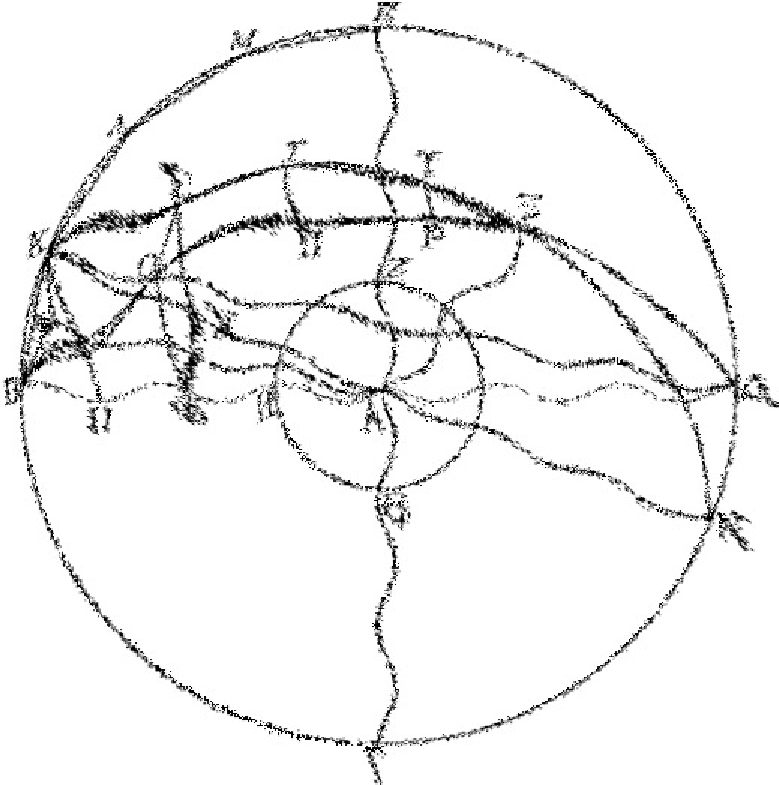
\includegraphics{Book12/front.pdf}}
\newpage

%%%%
%12.1
%%%%
\pdfbookmark[1]{Proposition 12.1}{pdf12.1}
\pagestyle{fancy}
\cfoot{\gr{\kern -.7pt }}
\lhead{\large\gr{ΣΤΟΙΘΕΙΩΝ \kern -.7pt {12}.}}
\rhead{\large ELEMENTS BOOK 12}
\begin{Parallel}{}{}
\ParallelLText{
\begin{center}
{\large \ggn{1}.}
\end{center}\vspace*{-7pt}

\gr{Τὰ ἐν τοῖξ κύκλοιξ <όμοια πολύγωνα πρὸξ >άλληλά ἐστιν ὡξ τὰ
ἀπὸ τῶν διαμέτρων τετράγωνα.}

% Removed epsf size command
\centerline{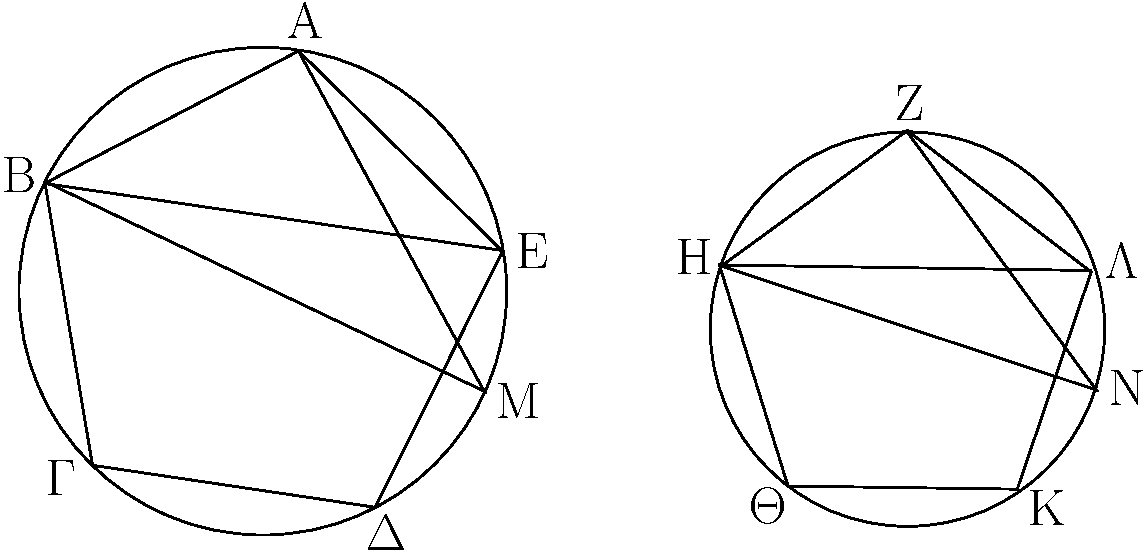
\includegraphics{Book12/fig01g.pdf}}

\gr{>'Εστωσαν κύκλοι οἱ ΑΒΓ, ΖΗΘ, καὶ ἐν α\kern -.7pt  ὐτοῖξ
<όμοια πολύγωνα >έστω τὰ ΑΒΓΔΕ, ΖΗΘΚΛ, διάμετροι
δὲ τῶν κύκλων >έστωσαν ΒΜ, ΗΝ; λέγω, <ότι ἐστὶν ὡξ τὸ ἀπὸ τῆξ
ΒΜ τετράγωνον πρὸξ τὸ ἀπὸ τῆξ ΗΝ τετράγωνον, ο<ύτωξ
τὸ ΑΒΓΔΕ πολύγωνον πρὸξ τὸ ΖΗΘΚΛ πολύγωνον.}

\gr{Ἐπεζεύθθωσαν γὰρ αἱ ΒΕ, ΑΜ, ΗΛ, ΖΝ. καὶ ἐπεὶ <όμοιον τὸ
ΑΒΓΔΕ πολύγωνον τῶ| ΖΗΘΚΛ πολυγώνῳ, >ίση ἐστὶ καὶ
ἡ ὑπὸ ΒΑΕ γωνία τῆ| ὑπὸ ΗΖΛ, καί ἐστιν ὡξ ἡ ΒΑ
πρὸξ τὴν ΑΕ, ο<ύτωξ ἡ ΗΖ πρὸξ τὴν ΖΛ. δύο δὴ τρίγωνά ἐστι
τὰ ΒΑΕ, ΗΖΛ μίαν γωνίαν μιᾶ| γωνίᾳ >ίσην >έθοντα τὴν ὑπὸ
ΒΑΕ τῆ| ὑπὸ ΗΖΛ, περὶ δὲ τὰξ >ίσαξ γωνίαξ τὰξ πλευρὰξ
ἀνάλογον; ἰσογώνιον >άρα ἐστὶ τὸ ΑΒΕ τρίγωνον τῶ| ΖΗΛ τριγώνῳ.
>ίση >άρα ἐστὶν ἡ ὑπὸ ΑΕΒ γωνία τῆ| ὑπὸ ΖΛΗ. ἀλλ> ἡ μὲν
ὑπὸ ΑΕΒ τῆ| ὑπὸ ΑΜΒ ἐστιν >ίση; ἐπὶ γὰρ τῆξ α\kern -.7pt  ὐτῆξ
περιφερείαξ βεβήκασιν; ἡ δὲ ὑπὸ ΖΛΗ τῆ| ὑπὸ ΖΝΗ; καὶ ἡ
ὑπὸ ΑΜΒ >άρα τῆ| ὑπὸ ΖΝΗ ἐστιν >ίση. >έστι δὲ καὶ ὀρθὴ
ἡ ὑπὸ ΒΑΜ ὀρθῆ| τῆ| ὑπὸ ΗΖΝ >ίση; καὶ ἡ λοιπὴ >άρα
τῆ| λοιπῆ| ἐστιν >ίση. ἰσογώνιον >άρα ἐστὶ τὸ ΑΒΜ τρίγωνον
τῶ| ΖΗΝ τρίγωνῳ. ἀνάλογον >άρα ἐστὶν ὡξ ἡ ΒΜ πρὸξ τὴν
ΗΝ, ο<ύτωξ ἡ ΒΑ πρὸξ τὴν ΗΖ. ἀλλὰ τοῦ μὲν τῆξ ΒΜ πρὸξ
τὴν ΗΝ λόγον διπλασίων ἐστὶν ὁ τοῦ ἀπὸ τῆξ ΒΜ τετραγώνου
πρὸξ τὸ ἀπὸ τῆξ ΗΝ τετράγωνον, τοῦ δὲ τῆξ ΒΑ πρὸξ τὴν
ΗΖ διπλασίων ἐστὶν ὁ τοῦ ΑΒΓΔΕ πολυγώνου πρὸξ τὸ ΖΗΘΚΛ
πολύγωνον; καὶ ὡξ >άρα τὸ ἁπὸ τῆξ ΒΜ τετράγωνον πρὸξ
τὸ ἀπὸ τῆξ ΗΝ τετράγωνον, ο<ύτωξ τὸ ΑΒΓΔΕ πολύγωνον
πρὸξ τὸ ΖΗΘΚΛ πολύγωνον.}

\gr{Τὰ >άρα ἐν τοῖξ κύκλοιξ <όμοια πολύγωνα πρὸξ >άλληλά ἐστιν ὡξ τὰ
ἀπὸ τῶν διαμέτρων τετράγωνα; <όπερ >έδει δεῖχαι.}}

\ParallelRText{
\begin{center}
{\large Proposition 1}
\end{center}

Similar polygons (inscribed) in circles are to one another
as the squares on the diameters (of the circles).

% Removed epsf size command
\centerline{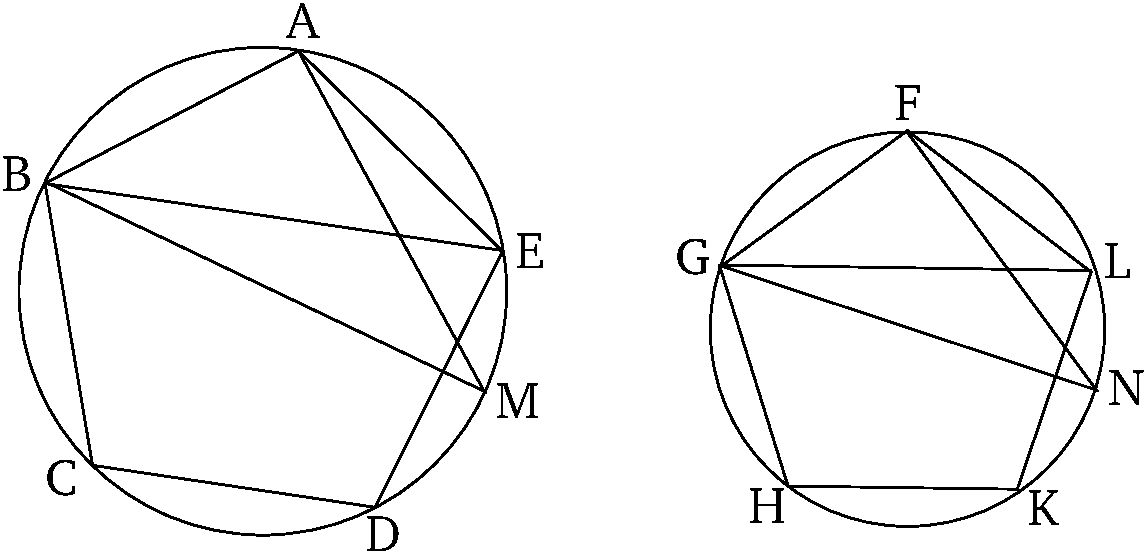
\includegraphics{Book12/fig01e.pdf}}

Let $ABC$ and $FGH$ be circles, and let $ABCDE$ and $FGHKL$ be
similar polygons (inscribed) in them (respectively), and let $BM$ and
$GN$ be the diameters of the circles (respectively). I say that as the square on
$BM$ is to the square on $GN$, so polygon $ABCDE$ (is) to polygon
$FGHKL$.

For let $BE$, $AM$, $GL$, and $FN$ be joined. And since polygon
$ABCDE$ (is) similar to polygon $FGHKL$, angle $BAE$ is also equal to
(angle) $GFL$, and as $BA$ is to $AE$, so $GF$ (is) to  $FL$ [Def.~6.1]. So, $BAE$ and $GFL$ are two triangles having one angle
equal to one angle, (namely), $BAE$ (equal) to $GFL$, and the sides
around the equal angles proportional. Triangle $ABE$ is thus equiangular with
triangle $FGL$ [Prop.~6.6]. Thus, angle $AEB$ is equal to
(angle) $FLG$. But, $AEB$ is equal to $AMB$, and $FLG$ to $FNG$, for they stand on the same
circumference [Prop.~3.27].
Thus, $AMB$ is also equal to $FNG$. And the right-angle $BAM$ is also
equal to the right-angle $GFN$ [Prop.~3.31]. 
Thus, the remaining (angle) is also equal to the remaining (angle) [Prop.~1.32]. Thus,
triangle $ABM$ is equiangular with triangle $FGN$. Thus, proportionally, as $BM$
is to $GN$, so $BA$ (is) to $GF$ [Prop.~6.4]. But, 
the (ratio) of the square on $BM$ to the square
on $GN$ is the square of the
ratio of $BM$ to $GN$, and  the (ratio) of
polygon $ABCDE$ to polygon $FGHKL$ is the square of the (ratio) of $BA$ to $GF$ [Prop.~6.20].  
And, thus, as the square on $BM$ (is) to the square on $GN$, so polygon $ABCDE$
(is) to polygon $FGHKL$. 

Thus, similar polygons (inscribed) in circles are to one another
as the squares on the diameters (of the circles). (Which is) the very thing it was required to
show.}
\end{Parallel}

%%%%
%12.2
%%%%
\pdfbookmark[1]{Proposition 12.2}{pdf12.2}
\begin{Parallel}{}{}
\ParallelLText{
\begin{center}
{\large \ggn{2}.}
\end{center}\vspace*{-7pt}

\gr{Οἱ κύκλοι πρὸξ ἀλλήλουξ εἰσὶν ὡξ τὰ ἀπὸ τῶν διαμέτρων τετράγωνα.}

\gr{>'Εστωσαν κύκλοι οἱ ΑΒΓΔ, ΕΖΗΘ, διάμετροι δὲ α\kern -.7pt  ὐτῶν [>έστωσαν]
αἱ ΒΔ, ΖΘ; λέγω, <ότι ἐστὶν ὡξ ὁ ΑΒΓΔ κύκλοξ πρὸξ τὸν ΕΖΗΘ
κύκλον, ο<ύτωξ τὸ ἀπὸ τῆξ ΒΔ τετράγωνον πρὸξ τὸ ἀπὸ τῆξ ΖΘ
τετράγωνον.}

% Removed epsf size command
\centerline{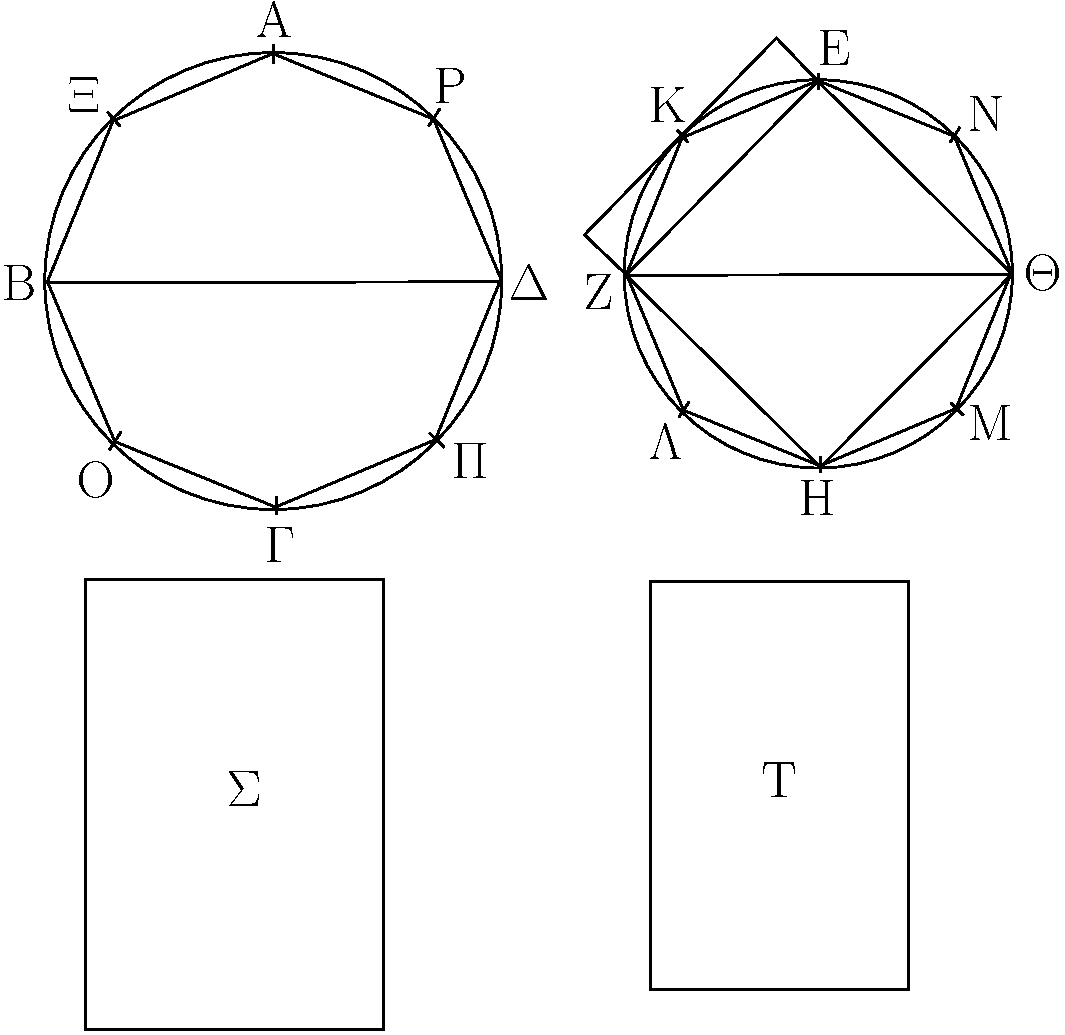
\includegraphics{Book12/fig02g.pdf}}

\gr{Εἰ γὰρ μ\kern -.7pt  ή ἐστιν ὡξ ὁ ΑΒΓΔ κύκλοξ πρὸξ τὸν ΕΖΗΘ, ο<ύτωξ τὸ ἀπὸ
τῆξ ΒΔ τετράγωνον πρὸξ τὸ ἀπὸ τῆξ ΖΘ, >έσται ὡξ τὸ ἀπὸ τῆξ
ΒΔ πρὸξ τὸ ἀπὸ τῆξ ΖΘ, ο<ύτωξ ὁ ΑΒΓΔ κύκλοξ >ήτοι πρὸξ >έλασσόν
τι τοῦ ΕΖΗΘ κύκλου θωρίον >ὴ πρὸξ μεῖζον. >έστω πρότερον πρὸξ
>έλασσον τὸ Σ. και ἐγγεγράφθω εἰξ τὸν ΕΖΗΘ κύκλον τετράγωνον τὸ
ΕΖΗΘ. τὸ δὴ ἐγγεγραμμένον τετράγωνον μεῖζόν ἐστιν >ὴ 
τὸ <ήμισυ τοῦ ΕΖΗΘ κύκλου, ἐπειδήπερ ἒαν  διὰ τῶν Ε, Ζ, Η, Θ
σημείων ἐφαπτομέναξ [εὐθείαξ] τοῦ κύκλου ἀγάγωμεν, τοῦ 
περιγραφομένου περὶ τὸν κύκλον τετραγώνου <ήμισύ ἐστι  τὸ ΕΖΗΘ τετράγωνον,
τοῦ δὲ  περιγραφέντοξ τετραγώνου ἐλάττων ἐστὶν ὁ κύκλοξ; <ώστε τὸ
ΕΖΗΘ  ἐγγεγραμμένομ\kern -.7pt  ῆν τετράγωνον μεῖζόν ἐστι τοῦ 
ἡμίσεωξ τοῦ ΕΖΗΘ κύκλου. τετμ\kern -.5pt  ήσθωσαν δίθα αἱ ΕΖ, ΖΗ, ΗΘ, ΘΕ περιφέρειαι κατὰ
τὰ Κ, Λ, Μ, Ν σημεῖα, καὶ ἐπεζεύθθωσαν αἱ ΕΚ, ΚΖ, ΖΛ, ΛΗ, ΗΜ, ΜΘ, ΘΝ, ΝΕ;
καὶ <έκαστον >άρα τῶν ΕΚΖ, ΖΛΗ, ΗΜΘ, ΘΝΕ τριγώνων μεῖζόν ἐστιν
>ὴ τὸ <ήμισυ τοῦ καθ> ἑαυτὸ τμ\kern -.3pt  ήματοξ τοῦ κύκλου, ἐπειδήπερ
ἒαν διὰ τῶν Κ, Λ, Μ, Ν σημείων ἐφαπτομέναξ τοῦ κύκλου ἀγάγωμεν
καὶ ἀναπληρώσωμεν τὰ ἐπὶ τῶν ΕΖ, ΖΗ, ΗΘ, ΘΕ εὐθειῶν παραλληλόγραμμα,
<έκαστον τῶν ΕΚΖ, ΖΛΗ, ΗΜΘ, ΘΝΕ τριγώνων <ήμισυ >έσται τοῦ καθ> ἑαυτὸ
παραλληλογράμμου, ἀλλὰ τὸ καθ> ἑαυτὸ τμ\kern -.7pt  ῆμα >έλαττόν ἐστι τοῦ
παραλληλογράμμου; <ώστε <έκαστον τῶν ΕΚΖ, ΖΛΗ, ΗΜΘ, ΘΝΕ
τριγώνων μεῖζόν ἐστι τοῦ ἡμίσεωξ τοῦ καθ> ἑαυτὸ τμ\kern -.7pt  ήματοξ
τοῦ κύκλου. τέμνοντεξ δὴ τὰξ ὑπολειπομέναξ περιφερείαξ δίθα καὶ
ἐπιζευγνύντεξ εὐθείαξ καὶ τοῦτο ἀεὶ ποιοῦντεξ καταλείψομέν τινα ἀποτμ\kern -.7pt  ήματα
τοῦ κύκλου, <ὰ >έσται ἐλάσσονα τῆξ ὑπεροθῆξ, <ῆ| ὑπερέθει ὁ ΕΖΗΘ
κύκλοξ τοῦ Σ θωρίου. ἐδείθθη γὰρ ἐν τῶ| πρώτῳ θεωρήματι τοῦ δεκάτου
βιβλίου, <ότι δύο μεγεθῶν ἀνίσων ἐκκειμένων, ἒαν ἀπὸ τοῦ μείζονοξ
ἀφαιρεθῆ| μεῖζον >ὴ τὸ <ήμισυ καὶ τοῦ καταλειπομένου μεῖζον >ὴ
τὸ <ήμισυ, καὶ τοῦτο ἀεὶ γίγνηται, λειφθήσεταί τι μέγεθοξ, <ὸ >έσται >έλασσον
τοῦ ἐκκειμένου ἐλάσσονοξ μεγέθουξ. λελείφθω ο>ῦν, καὶ >έστω τὰ ἐπὶ
τῶν ΕΚ, ΚΖ, ΖΛ, ΛΗ, ΗΜ, ΜΘ, ΘΝ, ΝΕ τμ\kern -.7pt  ήματα τοῦ ΕΖΗΘ κύκλου ἐλάττονα
τῆξ ὑπεροθῆξ, <ῆ| ὑπερέθει ὁ ΕΖΗΘ κύκλοξ τοῦ Σ θωρίου. λοιπὸν >άρα τὸ ΕΚΖΛΗΜΘΝ πολύγωνον
μεῖζόν ἐστι τοῦ Σ θωρίου.
 ἐγγεγράφθω καὶ εἰξ τὸν ΑΒΓΔ κύκλον τῶ| ΕΚΖΛΗΜΘΝ
πολυγώνῳ <όμοιον πολύγωνον τὸ ΑΧΒΟΓΠΔΡ; >έστιν >άρα ὡξ τὸ ἀπὸ
τῆξ ΒΔ τετράγωνον πρὸξ τὸ ἀπὸ τῆξ ΖΘ τετράγωνον, ο<ύτωξ τὸ
ΑΧΒΟΓΠΔΡ πολύγωνον πρὸξ τὸ ΕΚΖΛΗΜΘΝ πολύγωνον. ἀλλὰ καὶ ὡξ  τὸ ἀπὸ τῆξ ΒΔ τετράγωνον πρὸξ τὸ ἀπὸ τῆξ
ΖΘ, ο<ύτωξ ὁ ΑΒΓΔ κύκλοξ πρὸξ τὸ Σ θωρίον; καὶ ὡξ >άρα ὁ ΑΒΓΔ κύκλοξ
πρὸξ τὸ Σ θωρίον, ο<ύτωξ τὸ ΑΧΒΟΓΠΔΡ πολύγωνον πρὸξ τὸ ΕΚΖΛΗΜΘΝ
πολύγωνον; ἐναλλὰχ >άρα ὡξ ὁ ΑΒΓΔ κύκλοξ πρὸξ τὸ ἐν α\kern -.7pt  ὐτῶ| πολύγωνον, ο<ύτωξ τὸ Σ θωρίον πρὸξ τὸ ΕΚΖΛΗΜΘΝ πολύγωνον.  μείζων δὲ ὁ ΑΒΓΔ κύκλοξ τοῦ ἐν α\kern -.7pt  ὐτῶ| πολυγώνου; μεῖζον >άρα καὶ τὸ Σ θωρίον τοῦ ΕΚΖΛΗΜΘΝ πολυγώνου. ἀλλὰ
καὶ >έλαττον; <όπερ ἐστὶν ἀδύνατον. οὐκ >άρα ἐστὶν ὡξ τὸ ἀπὸ τῆξ ΒΔ τετράγωνον πρὸξ τὸ ἀπὸ τῆξ ΖΘ, ο<ύτωξ ὁ ΑΒΓΔ κύκλοξ πρὸξ >έλασσόν τι τοῦ ΕΖΗΘ κύκλου θωρίον. ὁμοίωξ δὴ δείχομεν, <ότι οὐδὲ ὡξ τὸ ἀπὸ ΖΘ πρὸξ
τὸ ἀπὸ ΒΔ, ο<ύτωξ ὁ ΕΖΗΘ κύκλοξ πρὸξ >έλασσόν τι τοῦ ΑΒΓΔ κύκλου θωρίον.}

\gr{Λέγω δή, <ότι οὐδὲ ὡξ τὸ ἀπὸ τῆξ ΒΔ πρὸξ τὸ ἀπὸ τῆξ ΖΘ, ο<ύτωξ
ὁ ΑΒΓΔ κύκλοξ πρὸξ μεῖζόν τι τοῦ ΕΖΗΘ κύκλου θωρίον.}

\gr{Εἰ γὰρ δυνατόν, >έστω πρὸξ μεῖζον τὸ Σ. ἀνάπαλιν >άρα [ἐστὶν]
ὡξ τὸ ἀπὸ τῆξ ΖΘ τετράγωνον πρὸξ τὸ ἀπὸ τῆξ ΔΒ, ο<ύτωξ τὸ Σ
θωρίον πρὸξ τὸν ΑΒΓΔ κύκλον. ἀλλ> ὡξ τὸ Σ θωρίον πρὸξ τὸν ΑΒΓΔ
κύκλον, ο<ύτωξ ὁ ΕΖΗΘ κύκλοξ πρὸξ >έλαττόν τι τοῦ ΑΒΓΔ κύκλου θωρίον; καὶ
ὡξ >άρα τὸ ἀπὸ τῆξ ΖΘ πρὸξ τὸ ἀπὸ τῆξ ΒΔ, ο<ύτωξ ὁ ΕΖΗΘ κύκλοξ
πρὸξ >έλασσόν τι τοῦ ΑΒΓΔ κύκλου θωρίον; <όπερ ἀδύνατον ἐδείθθη. οὐκ
>άρα ἐστὶν ὡξ τὸ ἀπὸ τῆξ ΒΔ τετράγωνον πρὸξ τὸ ἀπὸ τῆξ ΖΘ, ο<ύτωξ
ὁ ΑΒΓΔ κύκλοξ πρὸξ μεῖζόν τι τοῦ ΕΖΗΘ κύκλου θωρίον. ἐδείθθη
δέ, <ότι οὐδὲ πρὸξ >έλασσον; >έστιν >άρα ὡξ τὸ ἀπὸ τῆξ ΒΔ τετράγωνον
πρὸξ τὸ ἀπὸ τῆξ ΖΘ, ο<ύτωξ ὁ ΑΒΓΔ κύκλοξ πρὸξ τὸν ΕΖΗΘ κύκλον.}

\gr{Οἱ >άρα κύκλοι πρὸξ ἀλλήλουξ εἰσὶν ὡξ τὰ ἀπὸ τῶν διαμέτρων τετράγωνα;
<όπερ >έδει δεῖχαι.}}

\ParallelRText{
\begin{center}
{\large Proposition 2}
\end{center}

Circles are to one another as the squares on (their) diameters.

Let $ABCD$ and $EFGH$ be circles, and [let] $BD$ and $FH$ [be] their diameters.
I say that as circle $ABCD$ is to circle $EFGH$, so the square on $BD$ (is)
to the square on $FH$.\\

% Removed epsf size command
\centerline{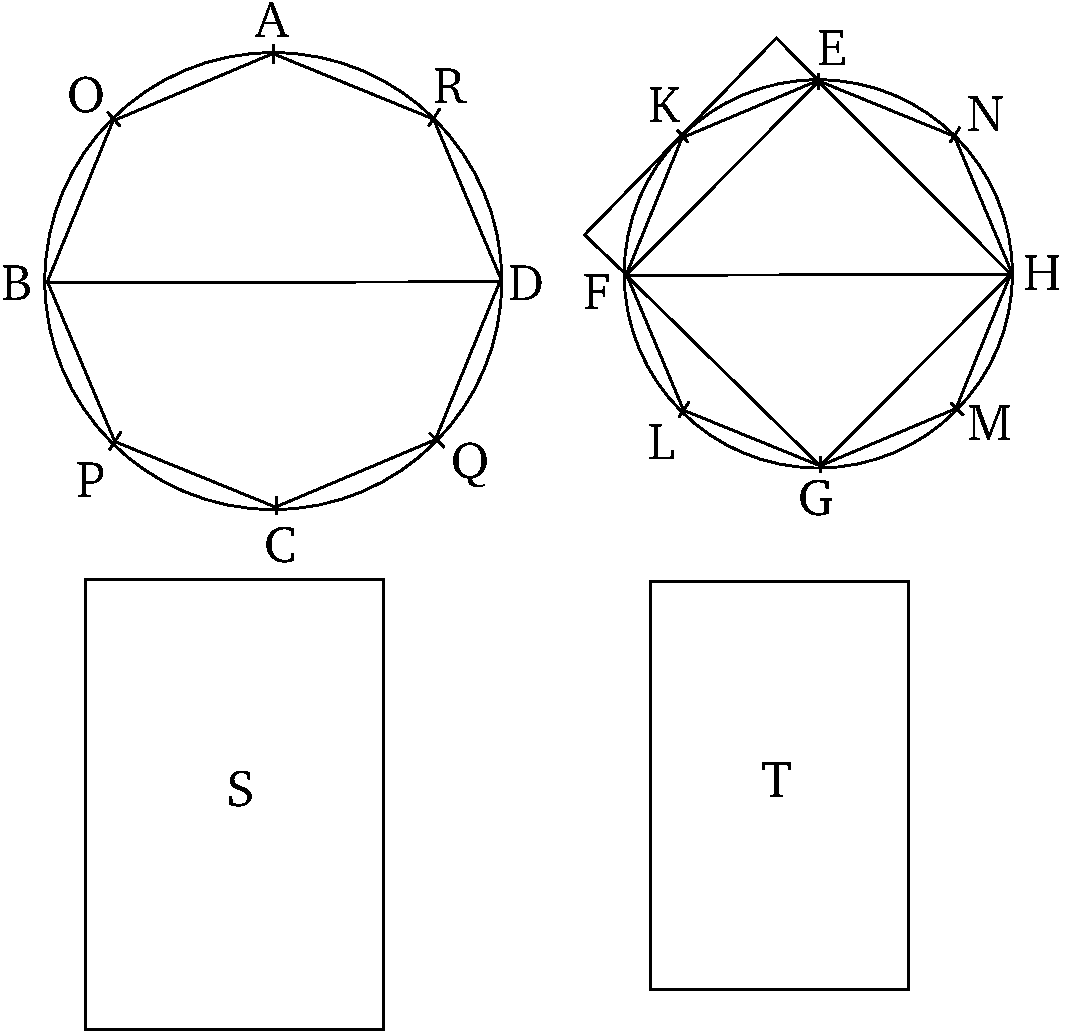
\includegraphics{Book12/fig02e.pdf}}

For if the circle $ABCD$ is not to the (circle) $EFGH$, as the square on
$BD$ (is) to the (square) on $FH$, then  as the (square) on $BD$ (is) to
the (square) on $FH$, so circle $ABCD$ will be to some area either less than, or greater
than, circle $EFGH$. Let it, first of all, be (in that ratio) to (some) lesser (area), $S$.
And let the square $EFGH$ be inscribed in circle $EFGH$ [Prop.~4.6]. So the inscribed
square is greater than half of circle $EFGH$, inasmuch as if we draw tangents to the circle through the points $E$, $F$, $G$, and $H$,
then square $EFGH$ is half of the square circumscribed about the circle [Prop.~1.47], and the circle is less than the
circumscribed square. Hence, the inscribed square $EFGH$ is greater than
half of circle $EFGH$. Let the circumferences $EF$, $FG$, $GH$,
and $HE$ be cut in half at points $K$, $L$, $M$, and $N$ (respectively), and let $EK$, $KF$, $FL$, $LG$, $GM$, $MH$, $HN$,
and $NE$ be joined. And, thus, each of the triangles
$EKF$, $FLG$, $GMH$, and $HNE$ is greater than half of the
segment of the circle about it, inasmuch as if we draw tangents to the circle through points $K$, $L$, $M$, and $N$, and complete the parallelograms on the straight-lines $EF$, $FG$, $GH$, and $HE$, then
each of the triangles $EKF$, $FLG$, $GMH$, and $HNE$ will be
half of the parallelogram about it, but the segment about
it is less than the parallelogram. Hence, each of the triangles $EKF$, 
$FLG$, $GMH$, and $HNE$ is greater than half of the segment of
the circle about it. So, by cutting the  circumferences remaining behind in half,
and joining straight-lines, and doing this continually, we will
(eventually) leave behind some segments of the circle whose (sum) will be
less than the excess by which circle $EFGH$ exceeds the area $S$.
For we showed in the first theorem of the tenth book that if two unequal
magnitudes are laid out, and if (a part) greater than a half is subtracted
from the greater, and (if from) the remainder (a part) greater than a
half (is subtracted), and this happens continually, then some magnitude
will (eventually) be left which will be less than the lesser laid out magnitude [Prop.~10.1]. Therefore, let the (segments) be left, and let 
 the (sum of the) segments of the circle $EFGH$ on $EK$, $KF$, $FL$, $LG$, $GM$, $MH$, $HN$, and $NE$ be less than the excess by which  circle
 $EFGH$ exceeds  area $S$. Thus, the remaining polygon $EKFLGMHN$ is greater than area $S$. 
 And let the polygon $AOBPCQDR$,
 similar to the polygon $EKFLGMHN$, be inscribed in circle
 $ABCD$. Thus, as the square on $BD$ is to the square on $FH$, so
polygon $AOBPCQDR$ (is) to polygon $EKFLGMHN$ [Prop.~12.1]. But, also, as the square on $BD$ (is) to the square on $FH$, so circle $ABCD$ (is) to area $S$. And, thus, as
circle $ABCD$ (is) to area $S$, so polygon $AOBPGQDR$ (is) to
polygon $EKFLGMHN$ [Prop.~5.11]. Thus, alternately, as circle $ABCD$
(is) to the polygon (inscribed) within it, so area $S$ (is) to polygon $EKFLGMHN$
[Prop.~5.16]. And circle $ABCD$ (is)
greater than the polygon (inscribed) within it. Thus, area $S$ is also greater than polygon 
$EKFLGMHN$. But, (it is) also less. The very thing
is impossible. Thus, the square on $BD$ is not to the (square) on $FH$, as
circle $ABCD$ (is) to some area less than circle $EFGH$. So, similarly,
we can show that the (square) on $FH$ (is) not to the (square) on 
$BD$ as circle $EFGH$ (is) to some area less than circle $ABCD$ either.

So, I say that neither (is) the (square) on $BD$ to the (square) on $FH$,
as circle $ABCD$ (is) to some area greater than circle $EFGH$.

For, if possible, let it be (in that ratio) to (some)  greater (area), $S$. Thus, inversely, 
as the square on $FH$ [is] to the (square) on $DB$, so area $S$ (is) to circle $ABCD$ [Prop.~5.7~corr.]. But, as area $S$ (is) to circle $ABCD$, so circle $EFGH$
(is) to some area less than circle $ABCD$ (see lemma). And, thus, as the (square) on $FH$ (is) to the (square) on $BD$, so circle $EFGH$ (is) to some area
less than  circle $ABCD$ [Prop.~5.11]. The very thing was shown (to be) impossible.
Thus, as the square on $BD$ is to the (square) on $FH$, so circle $ABCD$
(is) not to some area greater than circle $EFGH$. And it was shown that neither (is it in that ratio) to (some) lesser (area). Thus, as the square on $BD$ is to the (square) on $FH$, so circle $ABCD$ (is) to circle $EFGH$.

Thus, circles are to one another as the squares on (their) diameters. (Which is) the very thing it was required to show.}
\end{Parallel}

\begin{Parallel}{}{}
\ParallelLText{
\begin{center}
{\large \gr{Λῆμμα}.}
\end{center}\vspace*{-7pt}

\gr{Λέγω δή, <ότι τοῦ Σ θωρίου μείζονοξ >όντοξ τοῦ ΕΖΗΘ κύκλου ἐστὶν ὡξ τὸ
Σ θωρίον πρὸξ τὸν ΑΒΓΔ κύκλον, ο<ύτωξ ὁ ΕΖΗΘ κύκλοξ πρὸξ >έλαττόν
τι τοῦ ΑΒΓΔ κύκλου θωρίον.}

\gr{Γεγονέτω γὰρ ὡξ τὸ Σ θωρίον πρὸξ τὸν ΑΒΓΔ κύκλον, ο<ύτωξ ὁ ΕΖΗΘ
κύκλοξ πρὸξ τὸ Τ θωρίον. λέγω, <ότι >έλαττόν ἐστι τὸ Τ θωρίον τοῦ
ΑΒΓΔ κύκλου. ἐπεὶ γάρ ἐστιν ὡξ τὸ Σ θωρίον πρὸξ τὸν ΑΒΓΔ
κύκλον, ο<ύτωξ ὁ ΕΖΗΘ κύκλοξ πρὸξ τὸ Τ θωρίον, ἐναλλάχ ἐστιν ὡξ τὸ
Σ θωρίον πρὸξ τὸν ΕΖΗΘ κύκλον, ο<ύτωξ ὁ ΑΒΓΔ κύκλοξ πρὸξ
τὸ Τ θωρίον. μεῖζον δὲ τὸ Σ θωρίον τοῦ ΕΖΗΘ κύκλου;
 μείζων >άρα καὶ ὁ ΑΒΓΔ κύκλοξ τοῦ
Τ θωρίου. <ώστε ἐστὶν ὡξ τὸ Σ θωρίον πρὸξ τὸν ΑΒΓΔ κύκλον, ο<ύτωξ
ὁ ΕΖΗΘ κύκλοξ πρὸξ >έλαττόν τι τοῦ ΑΒΓΔ κύκλου θωρίον;
<όπερ >έδει δεῖχαι.}}

\ParallelRText{
\begin{center}
\large{Lemma}
\end{center}

So, I say that, area $S$ being greater than circle $EFGH$, as area $S$ is to
circle $ABCD$, so circle $EFGH$ (is) to some area less
than circle $ABCD$.

For let it be contrived that as area $S$ (is) to circle $ABCD$,
so circle $EFGH$ (is) to area $T$. I say that area $T$ is less than circle
$ABCD$. For since as area $S$ is to circle $ABCD$, so circle $EFGH$
(is) to area $T$, alternately, as area $S$ is to circle $EFGH$, so circle
$ABCD$ (is) to area $T$ [Prop.~5.16]. And area $S$ (is) greater than circle $EFGH$.
Thus, circle $ABCD$ (is) also greater than area $T$ [Prop.~5.14]. Hence,
as area $S$ is to circle $ABCD$, so circle $EFGH$ (is) to some area less
than circle $ABCD$. (Which is) the very thing it was required to show.}
\end{Parallel}

%%%%
%12.3
%%%%
\pdfbookmark[1]{Proposition 12.3}{pdf12.3}
\begin{Parallel}{}{}
\ParallelLText{
\begin{center}
{\large \ggn{3}.}
\end{center}\vspace*{-7pt}

\gr{Πᾶσα πυραμὶξ τρίγωνον >έθουσα βάσιν διαιρεῖται εἰξ δύο πυραμίδαξ >ίσαξ
τε καὶ ὁμοίαξ ἀλλήλαιξ καὶ [ὁμοίαξ] τῆ| <όλῆ| τριγώνουξ ἐθουσαξ
βάσειξ καὶ εἰξ δύο πρίσματα >ίσα; καὶ τὰ δύο πρίσματα μείζονά ἐστιν
>ὴ τὸ <ήμισυ τῆξ <όληξ πυραμίδοξ.}\\

% Removed epsf size command
\centerline{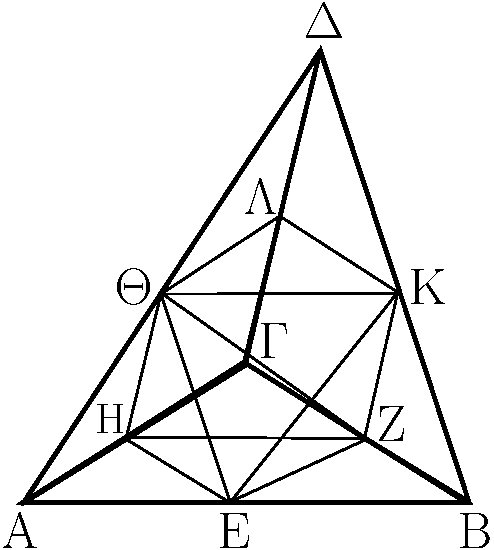
\includegraphics{Book12/fig03g.pdf}}

\gr{>'Εστω πυραμίξ, <ῆξ βάσιξ μέν ἐστι τὸ ΑΒΓ τρίγωνον, κορυφὴ δὲ τὸ
Δ σημεῖον; λέγω, <ότι ἡ ΑΒΓΔ πυραμὶξ διαιρεῖται εἰξ δύο πυραμίδαξ
>ίσαξ ἀλλήλαιξ τριγώνουξ βάσειξ ἐθούσαξ καὶ ὁμοίαξ τῆ| <όλῆ|
καὶ εἰξ δύο πρίσματα >ίσα; καὶ τὰ δύο πρίσματα μείζονά ἐστιν >ὴ
τὸ <ήμισυ τῆξ <όληξ πυραμίδοξ.}

\gr{Τετμ\kern -.7pt  ήσθωσαν γὰρ αἱ ΑΒ, ΒΓ, ΓΑ, ΑΔ, ΔΒ, ΔΓ δίθα κατὰ τὰ Ε, Ζ, Η, Θ, Κ, Λ
σημεῖα, καὶ ἐπεζεύθθωσαν αἱ ΘΕ, ΕΗ, ΗΘ, ΘΚ, ΚΛ, ΛΘ, ΚΖ,
ΖΗ. ἐπεὶ >ίση ἐστὶν ἡ μὲν ΑΕ τῆ| ΕΒ, ἡ δὲ ΑΘ τῆ| ΔΘ, παράλληλοξ
>άρα ἐστὶν ἡ ΕΘ τῆ| ΔΒ. διὰ τὰ α\kern -.7pt  ὐτὰ δὴ καὶ ἡ ΘΚ τῆ| ΑΒ παράλληλόξ
ἐστιν. παραλληλόγραμμον >άρα ἐστὶ τὸ ΘΕΒΚ; >ίση >άρα ἐστὶν ἡ
ΘΚ τῆ| ΕΒ. ἀλλὰ ἡ ΕΒ τῆ| ΕΑ ἐστιν >ίση; καὶ ἡ ΑΕ >άρα τῆ| ΘΚ ἐστιν
>ίση. >έστι δὲ καὶ ἡ ΑΘ τῆ| ΘΔ >ίση; δύο δὴ αἱ ΕΑ, ΑΘ δυσὶ ταῖξ ΚΘ,
ΘΔ >ίσαι εἰσὶν ἑκατέρα ἑκατέρᾳ; καὶ γωνία ἡ ὑπὸ ΕΑΘ γωνίᾳ
τῆ| ὑπὸ ΚΘΔ >ίση; βάσιξ >άρα ἡ ΕΘ βάσει τῆ| ΚΔ ἐστιν >ίση. >ίσον
>άρα καὶ <όμοιόν ἐστι τὸ ΑΕΘ τρίγωνον τῶ| ΘΚΔ τριγώνῳ. διὰ τὰ α\kern -.5pt  ὐτὰ
δὴ καὶ τὸ ΑΘΗ τρίγωνον τῶ| ΘΛΔ τριγώνῳ >ίσον τέ ἐστι καὶ <όμοιον.
καὶ ἐπεὶ δύο εὐθεῖαι ἁπτόμεναι ἀλλήλων αἱ ΕΘ, ΘΗ παρὰ δύο εὐθείαξ
ἁπτομέναξ ἀλλήλων τὰξ ΚΔ, ΔΛ εἰσιν οὐκ ἐν τῶ| α\kern -.3pt  ὐτῶ|
ἐπιπέδῳ ο>ῦσαι, >ίσαξ
γωνίαξ περιέχουσιν. >ίση >άρα ἐστὶν ἡ ὑπὸ ΕΘΗ γωνία τῆ| ὑπὸ
ΚΔΛ γωνίᾳ. καὶ ἐπεὶ δύο εὐθεῖαι αἱ ΕΘ, ΘΗ δυσὶ ταῖξ
ΚΔ, ΔΛ >ίσαι εἰσὶν ἑκατέρα εκατέρᾳ,  καὶ γωνία ἡ ὑπὸ ΕΘΗ γωνίᾳ τῆ|
ὑπὸ ΚΔΛ ἐστιν >ίση, βάσιξ >άρα ἡ ΕΗ βάσει τῆ| ΚΛ [ἐστιν] >ίση;
>ίσον >άρα καὶ <όμοιόν ἐστι τὸ ΕΘΗ τρίγωνον τῶ| ΚΔΛ τριγώνῳ. διὰ τὰ
α\kern -.7pt  ὐτὰ δὴ καὶ τὸ ΑΕΗ τρίγωνον τῶ| ΘΚΛ τριγώνῳ >ίσον τε καὶ <όμοιόν
ἐστιν. ἡ >άρα πυραμίξ, <ῆξ βάσιξ μέν ἐστι τὸ ΑΕΗ τρίγωνον, κορυφὴ
δὲ τὸ Θ σημεῖον, >ίση καὶ ὁμοία ἐστὶ πυραμίδι, <ῆξ
βάσιξ μέν ἐστι τὸ ΘΚΛ τρίγωνον, κορυφὴ δὲ τὸ Δ σημεῖον. καὶ ἐπεὶ
τριγώνου τοῦ ΑΔΒ παρὰ μίαν τῶν πλευρῶν τὴν ΑΒ >ῆκται ἡ ΘΚ, ἰσογώνιόν
ἐστι τὸ ΑΔΒ τρίγωνον τῶ| ΔΘΚ τριγώνῳ, καὶ τὰξ πλευρὰξ ἀνάλογον >έθουσιν;
<όμοιον >άρα ἐστὶ τὸ ΑΔΒ τρίγωνον τῶ| ΔΘΚ τριγώνῳ. διὰ τὰ α\kern -.7pt  ὐτὰ δὴ καὶ
τὸ μὲν ΔΒΓ τρίγωνον τῶ| ΔΚΛ τριγώνῳ <όμοιόν ἐστιν, τὸ δὲ ΑΔΓ
τῶ| ΔΛΘ. καὶ ἐπεὶ δύο εὐθεῖαι ἁπτόμεναι ἀλλήλων αἱ ΒΑ, ΑΓ παρὰ
δύο εὐθείαξ ἁπτομέναξ ἀλλήλων τὰξ ΚΘ, ΘΛ εἰσιν οὐκ ἐν τῶ|
α\kern -.7pt  ὐτῶ| ἐπιπέδῳ, >ίσαξ γωνίαξ περιέχουσιν. >ίση >άρα ἐστὶν ἡ ὑπὸ
ΒΑΓ γωνία τῆ| ὑπὸ ΚΘΛ. καί ἐστιν ὡξ ἡ ΒΑ πρὸξ τὴν ΑΓ, ο<ύτωξ
ἡ ΚΘ πρὸξ τὴν ΘΛ; <όμοιον >άρα ἐστὶ τὸ ΑΒΓ τρίγωνον τῶ| ΘΚΛ τριγώνῳ.
καὶ πυραμὶξ >άρα, <ῆξ βάσιξ μέν ἐστι τὸ ΑΒΓ τρίγωνον, κορυφὴ
δὲ τὸ Δ σημεῖον, ὁμοία ἐστὶ πυραμίδι, <ῆξ βάσιξ μέν ἐστι τὸ ΘΚΛ
τρίγωνον, κορυφὴ δὲ τὸ Δ σημεῖον. ἀλλὰ πυραμίξ, <ῆξ βάσιξ μέν
[ἐστι] τὸ ΘΚΛ τρίγωνον, κορυφὴ δὲ τὸ Δ σημεῖον, ὁμοία ἐδείθθη
πυραμίδι, <ῆξ βάσιξ μέν ἐστι τὸ ΑΕΗ τρίγωνον, κορυφὴ δὲ τὸ Θ σημεῖον.
ἑκατέρα >άρα τῶν ΑΕΗΘ, ΘΚΛΔ πυραμίδων ὁμοία ἐστὶ τῆ| <όλῃ
τῆ| ΑΒΓΔ πυραμίδι.}

\gr{Καὶ ἐπεὶ >ίση ἐστὶν ἡ ΒΖ τῆ| ΖΓ, διπλάσιόν ἐστι τὸ ΕΒΖΗ παραλληλόγραμμον τοῦ ΗΖΓ τριγώνου. καὶ ἐπεὶ, ἒαν >ῆ| δύο πρίσματα
ἰσο"υψῆ, καὶ τὸ μὲν >έθῃ βάσιν παραλληλόγραμμον, τὸ δὲ τρίγωνον,
διπλάσιον δὲ >ῆ| τὸ παραλληλόγραμμον τοῦ τριγώνου, >ίσα ἐστὶ τὰ
πρίσματα, >ίσον >άρα ἐστὶ τὸ πρίσμα τὸ περιεχόμενον ὑπὸ δύο μὲν
τριγώνων τῶν ΒΚΖ, ΕΘΗ, τριῶν δὲ παραλληλογράμμων τῶν ΕΒΖΗ, ΕΒΚΘ,
ΘΚΖΗ τῶ| πρισματι τῶ| περιεθομένῳ ὑπὸ δύο μὲν τριγώνων τῶν ΗΖΓ,
ΘΚΛ, τριῶν δὲ παραλληλογράμμων τῶν ΚΖΓΛ, ΛΓΗΘ, ΘΚΖΗ.
καὶ φανερόν, <ότι ἑκάτρον τῶν πρισμάτων, ο<ῦ τε βάσιξ τὸ ΕΒΖΗ παραλληλόγραμμον, ἀπεναντίον δὲ ἡ ΘΚ εὐθεῖα, καὶ ο<ῦ βάσιξ τὸ ΗΖΓ
τρίγωνον, ἀπεναντίον δὲ τὸ ΘΚΛ τρίγωνον, μεῖζόν ἐστιν ἑκατέραξ
τῶν πυραμίδων, <ῶν βάσειξ μὲν τὰ ΑΕΗ, ΘΚΛ τρίγωνα, κορυφαὶ,
δὲ τὰ Θ, Δ σημεῖα, ἐπειδήπερ [καί] ἒαν ἐπιζεύχωμεν τὰξ ΕΖ, ΕΚ
εὐθείαξ, τὸ μὲν πρίσμα, ο<ῦ βάσιξ τὸ ΕΒΖΗ παραλληλόγραμμον, 
ἀπεναντίον
δὲ ἡ ΘΚ εὐθεῖα, μεῖζόν ἐστι τῆξ πυραμίδοξ, <ῆξ βάσιξ τὸ ΕΒΖ
τρίγωνον, κορυφὴ δὲ τὸ Κ σημεῖον. ἀλλ> ἡ πυραμίξ, <ῆξ βάσιξ τὸ ΕΒΖ
τρίγωνον, κορυφὴ δὲ τὸ Κ σημεῖον, >ίση ἐστὶ πυραμίδι, <ῆξ βάσιξ
τὸ ΑΕΗ τρίγωνον, κορυφὴ δὲ τὸ Θ σημεῖον; ὑπὸ γὰρ
>ίσων καὶ ὁμοίων ἐπιπέδων περιέθονται. <ώστε καὶ τὸ πρίσμα,
ο<ῦ βάσιξ μὲν τὸ ΕΒΖΗ παραλληλόγραμμον, ἀπεναντίον δὲ ἡ ΘΚ εὐθεῖα,
μεῖζόν ἐστι πυραμίδοξ, <ῆξ  βάσιξ μὲν τὸ ΑΕΗ τρίγωνον, κορυφὴ
δὲ τὸ Θ σημεῖον. >ίσον δὲ τὸ μὲν πρίσμα, ο<ῦ βάσιξ τὸ ΕΒΖΗ παραλληλόγραμμον, ἀπεναντίον δὲ ἡ ΘΚ εὐθεῖα, τῶ| πρίσματι, ο<ῦ βάσιξ
μὲν τὸ ΗΖΓ τρίγωνον, ἀπεναντίον δὲ τὸ ΘΚΛ τρίγωνον; ἡ δὲ πυραμίξ,
<ῆξ βάσιξ τὸ ΑΕΗ τρίγωνον, κορυφὴ δὲ τὸ Θ σημεῖον, >ίση ἐστὶ πυραμίδι,
<ῆξ βάσιξ τὸ ΘΚΛ τρίγωνον, κορυφὴ δὲ τὸ Δ σημεῖον. τὰ >άρα εἰρημένα
δύο πρίσματα μείζονά ἐστι τῶν εἰρημένων δύο πυραμίδων, <ῶν βάσειξ
μὲν τὰ ΑΕΗ, ΘΚΛ τρίγωνα, κορυφαὶ δὲ τὰ Θ, Δ σημεῖα.}

\gr{Ἡ >άρα <όλη πυραμίξ, <ῆξ βάσιξ τὸ ΑΒΓ τρίγωνον, κορυφὴ δὲ τὸ Δ σημεῖον,
διή|ρηται ε>ίξ τε δύο πυραμίδαξ >ίσαξ ἀλλήλαιξ [καὶ ὁμοίαξ τῆ|
<όλῃ] καὶ εἰξ δύο πρίσματα >ίσα, καὶ τὰ δύο πρίσματα μείζονά ἐστιν
>ὴ τὸ <ήμισυ τῆξ <όληξ πυραμίδοξ; <όπερ >έδει δεῖχαι.}}

\ParallelRText{
\begin{center}
{\large Proposition 3}
\end{center}

Any pyramid having a triangular base is divided into two
pyramids having triangular bases (which are) equal, similar to one another, and [similar] to the whole, and into two equal prisms. And the (sum of the) two prisms is greater than half of the
whole pyramid.

% Removed epsf size command
\centerline{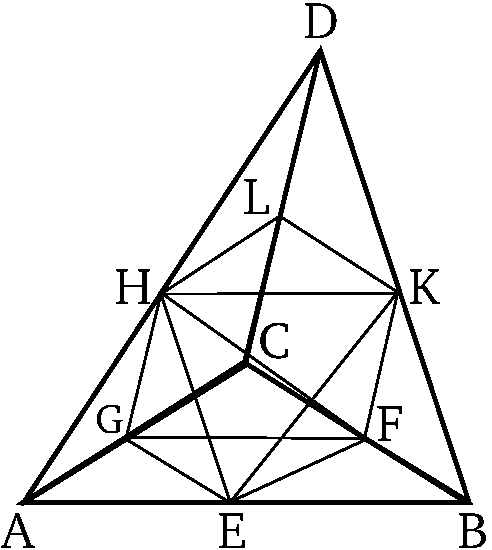
\includegraphics{Book12/fig03e.pdf}}

Let there be a pyramid whose base is triangle $ABC$, and (whose) apex (is) point $D$. I say that
pyramid $ABCD$ is divided into two pyramids having triangular bases (which are) equal
to one another, and similar to the whole, and into two equal prisms. And the (sum of the)
two prisms is greater than half of the whole pyramid.

For let $AB$, $BC$, $CA$, $AD$, $DB$, and $DC$ be cut in half at points $E$, $F$, $G$,
$H$, $K$, and $L$ (respectively). And let $HE$, $EG$, $GH$, $HK$, $KL$, $LH$, $KF$, and $FG$
be joined. Since $AE$ is equal to $EB$, and $AH$ to $DH$, $EH$ is thus parallel to
$DB$ [Prop.~6.2]. So, for the same (reasons), $HK$ is also parallel
to $AB$. Thus, $HEBK$ is a parallelogram. Thus, $HK$ is equal to $EB$ [Prop.~1.34]. But, $EB$ is equal to $EA$. Thus, $AE$ is also equal to $HK$. And $AH$
is also equal to $HD$. So the two (straight-lines) $EA$ and $AH$ are equal to the two
(straight-lines) $KH$ and $HD$, respectively. And angle $EAH$ (is) equal to angle
$KHD$ [Prop.~1.29]. Thus, base $EH$ is equal to base $KD$ [Prop.~1.4]. Thus, triangle $AEH$ is equal and similar to triangle $HKD$
[Prop.~1.4]. So, for the same (reasons), triangle $AHG$
is also equal and similar to triangle $HLD$. And since $EH$ and $HG$ are two
straight-lines joining one another (which are respectively) parallel to two straight-lines
joining one another, $KD$ and $DL$, not being in the same plane, they will contain
equal angles [Prop.~11.10]. Thus, angle $EHG$ is equal to angle
$KDL$. And since the two straight-lines $EH$ and $HG$ are equal to the two straight-lines
$KD$ and $DL$, respectively, and angle $EHG$ is equal to angle $KDL$, base $EG$
[is] thus equal to base $KL$ [Prop.~1.4]. Thus, triangle $EHG$ is equal
and similar to triangle $KDL$. So, for the same (reasons), triangle $AEG$ is also equal and
similar to triangle $HKL$. Thus, the pyramid whose base is triangle $AEG$,
and apex the point $H$, is equal and similar to the pyramid whose base is triangle $HKL$,
and apex the point $D$ [Def.~11.10]. And since $HK$ has been drawn
parallel to one of the sides, $AB$, of triangle $ADB$, triangle $ADB$
is equiangular to triangle $DHK$ [Prop.~1.29], and they have proportional sides. Thus, triangle $ADB$ is similar to triangle $DHK$ [Def.~6.1].
So, for the same (reasons), triangle $DBC$ is also similar to triangle $DKL$, and
$ADC$ to $DLH$. And since two straight-lines joining one another, $BA$ and $AC$, are parallel
to two straight-lines joining one another, $KH$ and $HL$, not in the same plane, they will
contain equal angles [Prop.~11.10]. Thus, angle $BAC$ is equal
to (angle) $KHL$. And as $BA$ is to $AC$, so $KH$ (is) to $HL$. Thus, triangle $ABC$ is
similar to triangle $HKL$ [Prop.~6.6]. And, thus, the pyramid whose base is triangle $ABC$, and apex
the point $D$, is similar to the pyramid whose base is triangle $HKL$, and apex the point $D$ [Def.~11.9]. But,
the pyramid whose base [is] triangle $HKL$, and apex the point $D$, was shown (to be) similar
to the pyramid whose base is triangle $AEG$, and apex the point $H$. Thus, each of the pyramids
$AEGH$ and $HKLD$ is similar to the whole pyramid $ABCD$.

And since $BF$ is equal to $FC$, parallelogram $EBFG$ is double triangle $GFC$ [Prop.~1.41]. And since, if two prisms (have) 
equal heights, and the former has a parallelogram as a base, and the latter a triangle, and the parallelogram (is) double
the triangle, then the prisms are equal [Prop.~11.39],  the prism
contained by the two triangles $BKF$ and $EHG$, and the three parallelograms $EBFG$,
$EBKH$, and $HKFG$, is thus  equal to the prism contained by the two triangles $GFC$ and
$HKL$, and the three parallelograms $KFCL$, $LCGH$, and $HKFG$. And (it is) clear that
each of the prisms whose base (is) parallelogram $EBFG$, and opposite (side) straight-line
$HK$, and whose base (is) triangle $GFC$, and opposite (plane) triangle $HKL$, is greater than
each of the pyramids whose bases are triangles $AEG$ and $HKL$, and apexes the points
$H$ and $D$ (respectively), inasmuch as, if we [also] join the straight-lines
$EF$ and $EK$ then the prism whose base (is) parallelogram $EBFG$, and opposite
(side) straight-line $HK$, is greater than the pyramid whose base (is) triangle $EBF$,
and apex the point $K$. But the pyramid whose base (is) triangle $EBF$, and apex the point $K$,
is equal to the pyramid whose base is triangle $AEG$, and apex point $H$. For
they are contained by equal and similar planes. And, hence, the prism whose base (is)
parallelogram $EBFG$, and opposite (side) straight-line $HK$, is greater than the pyramid
whose base (is) triangle $AEG$, and apex the  point $H$. And the prism 
whose base is
parallelogram $EBFG$, and opposite (side) straight-line $HK$, (is) equal to the prism
whose base (is) triangle $GFC$, and opposite (plane) triangle $HKL$. And the pyramid whose
base (is) triangle $AEG$, and apex the  point $H$, is equal to the pyramid whose base (is) triangle
$HKL$, and apex the point $D$. Thus, the (sum of the) aforementioned
two prisms is greater than the (sum of the) aforementioned two pyramids, whose bases (are)
triangles $AEG$ and $HKL$, and apexes the points $H$ and $D$ (respectively).

Thus, the whole pyramid, whose base (is) triangle $ABC$, and apex the point $D$, has been
divided into two pyramids (which are) equal to one another [and similar to the whole],
and into two equal prisms. And the (sum of the) two prisms is greater than half of the
whole pyramid. (Which is) the very thing it was required to show.}
\end{Parallel}

%%%%
%12.4
%%%%
\pdfbookmark[1]{Proposition 12.4}{pdf12.4}
\begin{Parallel}{}{}
\ParallelLText{
\begin{center}
{\large \ggn{4}.}
\end{center}\vspace*{-7pt}

\gr{Ἐὰν >ῶσι δύο πυραμίδεξ ὑπὸ τὸ α\kern -.7pt  ὐτὸ <ύψοξ τριγώνουξ >έθουσαι βάσειξ, διαιρεθῆ|
δὲ ἑκατέρα α\kern -.7pt  ὐτῶν ε>ίξ τε δύο πυραμίδαξ >ίσαξ ἀλλήλαιξ καὶ ὁμοίαξ 
τῆ|
<όλῃ καὶ εἰξ δύο πρίσματα >ίσα, >έσται ὡξ ἡ τῆξ μιᾶξ πυραμίδοξ βάσιξ πρὸξ
τὴν τῆξ ἑτέραξ πυραμίδοξ βάσιν, ο<ύτωξ τὰ ἐν τῆ| μιᾶ| πυραμίδι πρίσματα πάντα
πρὸξ τὰ ἐν τῆ| ἑτάρᾳ πυραμίδι πρίσματα πάντα ἰσοπληθῆ|.}

\gr{>'Εστωσαν δύο πυραμίδεξ ὑπὸ τὸ α\kern -.7pt  ὐτὸ <ύψοξ τριγώνουξ >έθουσαι βάσειξ τὰξ ΑΒΓ,
ΔΕΖ, κορυφὰξ δὲ τὰ Η, Θ σημεῖα, καὶ διῃρήσθω ἑκατέρα α\kern -.7pt  ὐτῶν ε>ίξ τε δύο
πυραμίδαξ >ίσαξ ἀλλήλαιξ καὶ ὁμοίαξ τῆ| <όλῃ καὶ εἰξ δύο πρίσματα >ίσα; λέγω,
<ότι ἐστὶν ὡξ ἡ ΑΒΓ βάσιξ πρὸξ τὴν ΔΕΖ βάσιν, ο<ύτωξ τὰ ἐν τῆ| ΑΒΓΗ
πυραμίδι πρίσματα πάντα πρὸξ τὰ ἐν τῆ| ΔΕΖΘ πυραμίδι πρίσματα  ἰσοπληθῆ.}\\~\\

% Removed epsf size command
\centerline{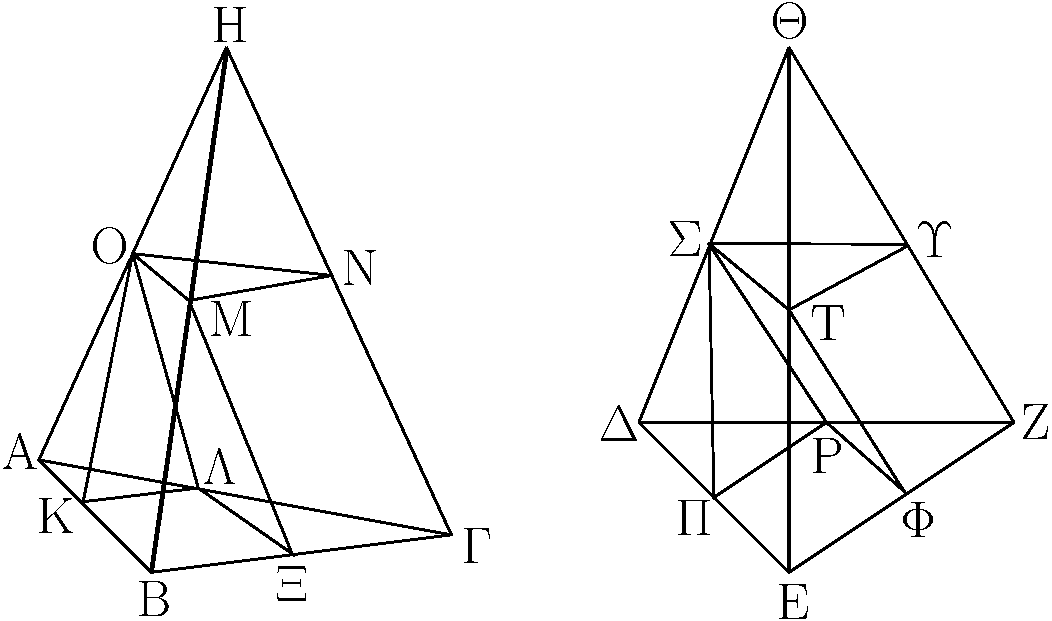
\includegraphics{Book12/fig04g.pdf}}

\gr{Ἐπεὶ γὰρ >ίση ἐστὶν ἡ μὲν ΒΧ τῆ| ΧΓ, ἡ δὲ ΑΛ τῆ| ΛΓ, παράλληλοξ >άρα ἐστὶν
ἡ ΛΧ τῆ| ΑΒ καὶ <όμοιον τὸ ΑΒΓ τρίγωνον τῶ| ΛΧΓ τριγώνῳ. διὰ τὰ α\kern -.7pt  ὐτὰ
δὴ καὶ τὸ ΔΕΖ τρίγωνον τῶ| ΡΦΖ τριγώνῳ <όμοιόν ἐστιν. καὶ ἐπεὶ διπλασίων
ἐστὶν ἡ μὲν ΒΓ τῆξ ΓΧ, ἡ δὲ ΕΖ τῆξ ΖΦ, >έστιν >άρα ὡξ ἡ ΒΓ πρὸξ
τὴν ΓΧ, ο<ύτωξ ἡ ΕΖ πρὸξ τὴν ΖΦ. καὶ ἀναγέγραπται ἀπὸ μὲν τῶν ΒΓ, ΓΧ
<όμοιά τε καὶ ὁμοίωξ κείμενα εὐθύγραμμα τὰ ΑΒΓ, ΛΧΓ, ἀπὸ δὲ τῶν
ΕΖ, ΖΦ <όμοιά τε καὶ ὁμοίωξ κείμενα [εὐθύγραμμα] τὰ ΔΕΖ, ΡΦΖ; 
>έστιν
>άρα ὡξ τὸ ΑΒΓ τρίγωνον πρὸξ τὸ ΛΧΓ τρίγωνον, ο<ύτωξ τὸ ΔΕΖ τρίγωνον
πρὸξ τὸ ΡΦΖ τρίγωνον; ἐναλλὰχ >άρα ἐστὶν ὡξ τὸ ΑΒΓ τρίγωνον πρὸξ
τὸ ΔΕΖ [τρίγωνον], ο<ύτωξ τὸ ΛΧΓ [τρίγωνον]
πρὸξ τὸ ΡΦΖ τρίγωνον. ἀλλ> ὡξ τὸ ΛΧΓ τρίγωνον πρὸξ τὸ ΡΦΖ τρίγωνον, ο<ύτωξ τὸ πρίσμα,
ο<ῦ βάσιξ μέν [ἐστι] τὸ ΛΧΓ τρίγωνον, ἀπεναντίον δὲ τὸ ΟΜΝ, πρὸξ τὸ πρίσμα, ο<ῦ
βάσιξ μὲν τὸ ΡΦΖ τρίγωνον, ἀπεναντίον δὲ τὸ ΣΤΥ; καὶ ὡξ >άρα τὸ ΑΒΓ τρίγωνον πρὸξ
τὸ ΔΕΖ τρίγωνον, ο<ύτωξ τὸ πρίσμα, ο<ῦ βάσιξ μὲν τὸ ΛΧΓ τρίγωνον, ἀπεναντίον
δὲ τὸ ΟΜΝ, πρὸξ τὸ πρίσμα, ο<ῦ βάσιξ μὲν τὸ ΡΦΖ τρίγωνον, ἀπεναντίον δὲ τὸ ΣΤΥ.
ὡξ δὲ τὰ εἰρημένα πρίσματα πρὸξ >άλληλα, ο<ύτωξ τὸ πρίσμα, ο<ῦ βάσιξ μὲν τὸ
ΚΒΧΛ παραλληλόγραμμον, ἀπεναντίον δὲ  ἡ ΟΜ εὐθεῖα, πρὸξ τὸ πρίσμα, ο<ῦ
βάσιξ μὲν τὸ ΠΕΦΡ παραλληλόγραμμον, ἀπεναντίον δὲ ἡ ΣΤ εὐθεῖα. καὶ τὰ δύο
>άρα πρίσματα, ο<ῦ τε βάσιξ μὲν τὸ ΚΒΧΛ
παραλληλόγραμμον, ἀπεναντίον δὲ ἡ ΟΜ, καὶ ο<ῦ βάσιξ μὲν τὸ ΛΧΓ, ἀπεναντίον δὲ τὸ
ΟΜΝ, πρὸξ τὰ πρίσματα, ο<ῦ τε βάσιξ μὲν τὸ ΠΕΦΡ, ἀπεναντίον δὲ ἡ ΣΤ εὐθεῖα,
καὶ ο~ὑ βάσιξ μὲν τὸ ΡΦΖ τρίγωνον, ἀπεναντίον δὲ τὸ ΣΤΥ. καὶ ὡξ >άρα
ἡ ΑΒΓ βάσιξ πρὸξ τὴν ΔΕΖ βάσιν, ο<ύτωξ τὰ  εἰρημένα δύο πρίσματα πρὸξ
τὰ εἰρημένα δύο πρίσματα.}

\gr{Καὶ ὁμοίωξ, ἒαν διαιρεθῶσιν αἱ ΟΜΝΗ, ΣΤΥΘ πυραμίδεξ ε>ίξ τε δύο πρίσματα καὶ δύο
πυραμίδαξ, >έσται ὡξ ἡ ΟΜΝ βάσιξ πρὸξ τὴν ΣΤΥ βάσιν,
ο<ύτωξ τὰ ἐν τῆ| ΟΜΝΗ πυραμίδι δύο πρίσματα πρὸξ τὰ ἐν τῆ| ΣΤΥΘ πυραμίδι δύο
πρίσματα. ἀλλ> ὡξ ἡ ΟΜΝ βάσιξ πρὸξ τὴν ΣΤΥ βάσιν, ο<ύτωξ ἡ ΑΒΓ βάσιξ
πρὸξ τὴν ΔΕΖ βάσιν; >ίσον γὰρ ἑκάτερον τῶν ΟΜΝ, ΣΤΥ τριγώνων ἑκατέρῳ
τῶν ΛΧΓ, ΡΦΖ. καὶ ὡξ >άρα ἡ ΑΒΓ βάσιξ πρὸξ τὴν ΔΕΖ βάσιν, ο<ύτωξ τὰ τέσσαρα
πρίσματα πρὸξ τὰ τέσσαρα πρίσματα. ὁμοίωξ δὲ κ>ὰν τὰξ ὑπολειπομέναξ πυραμίδαξ
διέλωμεν ε>ίξ τε δύο πυραμίδαξ καὶ εἰξ δύο πρίσματα, >έσται ὡξ ἡ
ΑΒΓ βάσιξ πρὸξ τὴν ΔΕΖ βάσιν, ο<ύτωξ τὰ ἐν τῆ| ΑΒΓΗ πυραμίδι πρίσματα πάντα πρὸξ
τὰ ἐν τῆ| ΔΕΖΘ πυραμίδι πρίσματα πάντα ἰσοπληθῆ; <όπερ >έδει δεῖχαι.}}

\ParallelRText{
\begin{center}
{\large Proposition 4}
\end{center}

If there are two pyramids with the same height, having trianglular
bases, and each of them is divided into two pyramids equal to one another, and
similar to the whole, and into two equal prisms then as the base of one pyramid
(is) to the base of the other pyramid, so  (the sum of) all the prisms in one pyramid
will be to (the sum of all) the equal  number of prisms in the other pyramid.

Let there be two pyramids with the same height, having the triangular
bases $ABC$ and $DEF$, (with)
apexes the points $G$ and $H$ (respectively). And let each of them be divided into
two pyramids equal to one another, and similar to the whole, and into two
equal prisms [Prop.~12.3]. I say that as base $ABC$ is to base
$DEF$, so (the sum of) all the prisms in pyramid $ABCG$ (is) to (the sum of) all the equal number of prisms in
pyramid $DEFH$.

% Removed epsf size command
\centerline{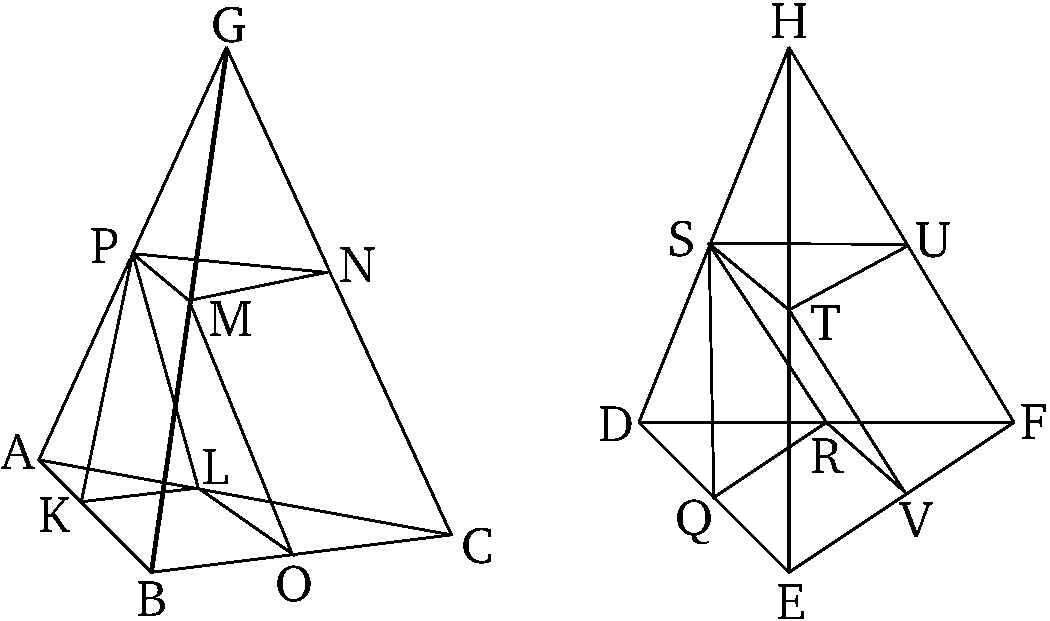
\includegraphics{Book12/fig04e.pdf}}

For since $BO$ is equal to $OC$, and $AL$ to $LC$,
$LO$ is thus parallel to $AB$, and triangle $ABC$ similar to triangle $LOC$
[Prop.~12.3]. So, for the same (reasons), triangle $DEF$ is also similar
to triangle $RVF$. And since $BC$ is double $CO$, and $EF$ (double) $FV$, thus
as $BC$ (is) to $CO$, so $EF$ (is) to $FV$. And the similar, and similarly laid out, rectilinear
(figures) $ABC$ and $LOC$ be described on $BC$ and $CO$ (respectively),
and the similar, and similarly laid out, [rectilinear] (figures) $DEF$ and $RVF$ on
$EF$ and $FV$ (respectively). Thus, as triangle $ABC$ is to triangle $LOC$, so triangle
$DEF$ (is) to triangle $RVF$ [Prop.~6.22]. Thus, alternately, as
triangle $ABC$ is to [triangle] $DEF$, so [triangle] $LOC$ (is) to triangle $RVF$ [Prop.~5.16]. But, as triangle $LOC$ (is) to triangle $RVF$, so the prism whose
base [is] triangle $LOC$, and opposite (plane) $PMN$, (is) to the prism whose base (is) triangle
$RVF$, and opposite (plane) $STU$ (see lemma). And, thus, as triangle $ABC$ (is) to triangle $DEF$,  so the prism whose base (is) triangle $LOC$, and opposite (plane) $PMN$, (is) to the
prism whose base (is) triangle $RVF$, and opposite (plane) $STU$. And as the aforementioned
prisms (are) to one another, so the prism whose base (is) parallelogram $KBOL$, and opposite
(side) straight-line $PM$, (is) to the prism whose
base (is) parallelogram $QEVR$, and opposite (side) straight-line $ST$ [Props.~11.39, 12.3]. Thus, also, (is) the (sum of the) two prisms---that whose base
(is) parallelogram $KBOL$, and opposite (side) $PM$, and that whose base (is) $LOC$,
and opposite (plane) $PMN$---to (the sum of) the  (two) prisms---that whose base (is) $QEVR$, and opposite
(side) straight-line $ST$, and that whose base (is) triangle $RVF$, and opposite (plane) $STU$
[Prop.~5.12]. And, thus, as base $ABC$ (is) to base $DEF$, so the 
(sum of the first) aforementioned two prisms (is) to the (sum  of the second) aforementioned two prisms.

And, similarly, if pyramids $PMNG$ and $STUH$ are divided into two prisms, and
two pyramids, as base $PMN$ (is) to base $STU$, so (the sum of) the  two prisms in pyramid
$PMNG$ will be to (the sum of) the  two prisms in pyramid $STUH$. But, as base $PMN$ (is) to
base $STU$, so base $ABC$ (is) to base $DEF$. For  the triangles $PMN$ and
$STU$ (are) equal to $LOC$ and $RVF$, respectively. And, thus, as base $ABC$ (is)
to base $DEF$, so (the sum of) the four prisms (is) to (the sum of) the four prisms [Prop.~5.12].
So, similarly, even if we  divide the pyramids left behind into two pyramids
and into two prisms, as base $ABC$ (is) to base $DEF$, so (the sum of) all the prisms in pyramid
$ABCG$ will be to (the sum of) all the equal number of prisms in pyramid $DEFH$. (Which is) the
very thing it was required to show.}
\end{Parallel}

\begin{Parallel}{}{}
\ParallelLText{
\begin{center}
\large{\gr{Λῆμμα}.}
\end{center}\vspace*{-7pt}

\gr{<'Οτι δέ ἐστιν ὡξ τὸ ΛΧΓ τρίγωνον πρὸξ τὸ ΡΦΖ τρίγωνον, ο<ύτωξ τὸ πρίσμα, ο<ῦ βάσιξ
τὸ ΛΧΓ τρίγωνον, ἀπεναντίον δὲ τὸ ΟΜΝ, πρὸξ τὸ πρίσμα, ο<ῦ
βάσιξ μὲν τὸ ΡΦΖ [τρίγωνον], ἀπεναντίον δὲ τὸ ΣΤΥ, ο<ύτω δεικτέον.}

\gr{Ἐπὶ γὰρ τῆξ α\kern -.7pt  ὐτῆξ καταγραφῆξ νενοήσθωσαν ἀπὸ τῶν Η, Θ κάθετοι
ἐπὶ τὰ ΑΒΓ, ΔΕΖ ἐπίπεδα, >ίσαι δηλαδὴ τυγθάνουσαι διὰ τὸ ἰσο"υψεῖξ ὑποκεῖσθαι
τὰξ πυραμίδαξ. καὶ ἐπεὶ δύο εὐθεῖαι <ή τε ΗΓ καὶ ἡ ἀπὸ τοῦ Η κάθετοξ
ὑπὸ παραλλήλων ἐπιπέδων τῶν ΑΒΓ, ΟΜΝ τέμνονται, εἰξ τοὺξ α\kern -.7pt  ὐτοὺξ
λόγουξ τμ\kern -.5pt  ηθήσονται. καὶ τέτμ\kern -.3pt  ηται ἡ ΗΓ δίθα ὑπὸ τοῦ ΟΜΝ ἐπιπέδου
κατὰ τὸ Ν; καὶ ἡ ἀπὸ τοῦ Η >άρα κάθετοξ ἐπὶ τὸ ΑΒΓ ἐπίπεδον δίθα τμ\kern -.7pt  ηθήσεται
ὑπὸ τοῦ ΟΜΝ ἐπιπέδου. διὰ τὰ α\kern -.7pt  ὐτὰ δὴ καὶ ἡ ἀπὸ τοῦ Θ κάθετοξ
ἐπὶ τὸ ΔΕΖ ἐπίπεδον δίθα τμ\kern -.7pt  ηθήσεται ὑπὸ τοῦ ΣΤΥ
ἐπιπέδου. καί εἰσιν >ίσαι αἱ ἀπὸ τῶν Η, Θ κάθετοι ἐπὶ τὰ ΑΒΓ, ΔΕΖ ἐπίπεδα;
>ίσαι >άρα καὶ αἱ ἀπὸ τῶν ΟΜΝ, ΣΤΥ τριγώνων ἐπὶ τὰ ΑΒΓ, ΔΕΖ
κάθετοι. ἰσο"υψῆ >άρα [ἐστὶ] τὰ πρίσματα, <ῶν βάσειξ μέν εἰσι τὰ ΛΧΓ, ΡΦΖ τρίγωνα,
ἀπεναντίον δὲ τὰ ΟΜΝ, ΣΤΥ. <ώστε καὶ τὰ στερεὰ παραλληλεπίπεδα τὰ ἀπὸ τῶν
εἰρημένων πρισμάτων ἀναγραφόμενα ἰσο"υψῆ καὶ πρὸξ >άλληλά [εἰσιν] ὡξ αἱ βάσειξ;
καὶ τὰ ἡμίση >άρα ἐστὶν ὡξ ἡ ΛΧΓ βάσιξ πρὸξ τὴν ΡΦΖ βάσιν, ο<ύτωξ τὰ εἰρημένα
πρίσματα πρὸξ >άλληλα; <όπερ >έδει δεῖχαι.}}

\ParallelRText{
\begin{center}
\large{Lemma}
\end{center}

And one may show, as follows, that as triangle $LOC$ is to triangle $RVF$, so the prism whose base (is) triangle $LOC$,
and opposite (plane) $PMN$, (is) to the prism whose base (is) [triangle] $RVF$, and opposite
(plane) $STU$. 

For, in the same figure, let perpendiculars be conceived (drawn) from (points)
$G$ and $H$ to the planes $ABC$ and $DEF$ (respectively). These clearly turn
out to be equal, on account of the pyramids being assumed (to be) of equal height. And
since two straight-lines, $GC$ and the perpendicular from $G$, are cut by the parallel
planes $ABC$ and $PMN$ they will be cut in the same ratios [Prop.~11.17]. And $GC$ was cut in half by the plane $PMN$ at $N$. Thus, the perpendicular
from $G$ to the plane $ABC$ will also be cut in half by the plane $PMN$. So, for the same
(reasons), the perpendicular from $H$ to the plane $DEF$ will also be cut in half by the
plane $STU$. And  the perpendiculars from $G$ and $H$ to the planes $ABC$ and $DEF$
(respectively) are equal. Thus, the perpendiculars from the triangles $PMN$ and $STU$
to $ABC$ and $DEF$ (respectively, are) also equal. Thus, the prisms whose bases are triangles
$LOC$ and $RVF$, and opposite (sides) $PMN$ and $STU$ (respectively), [are] of equal height.
And, hence, the parallelepiped solids described on the aforementioned prisms
[are] of equal height and (are) to one another as their bases [Prop.~11.32]. Likewise, the halves (of
the solids) [Prop.~11.28].  Thus, as base $LOC$ is to base $RVF$, so the
aforementioned prisms (are) to one another. (Which is) the very thing it was required to show.}
\end{Parallel}

%%%%
%12.5
%%%%
\pdfbookmark[1]{Proposition 12.5}{pdf12.5}
\begin{Parallel}{}{}
\ParallelLText{
\begin{center}
{\large \ggn{5}.}
\end{center}\vspace*{-7pt}

\gr{Αἱ ὑπὸ τὸ α\kern -.7pt  ὐτὸ <ύψοξ ο>ῦσαι πυραμίδεξ καὶ τριγώνουξ >έθουσαι βάσειξ πρὸξ ἀλλήλαξ
εἰσὶν ὡξ αἱ βάσειξ.}

% Removed epsf size command
\centerline{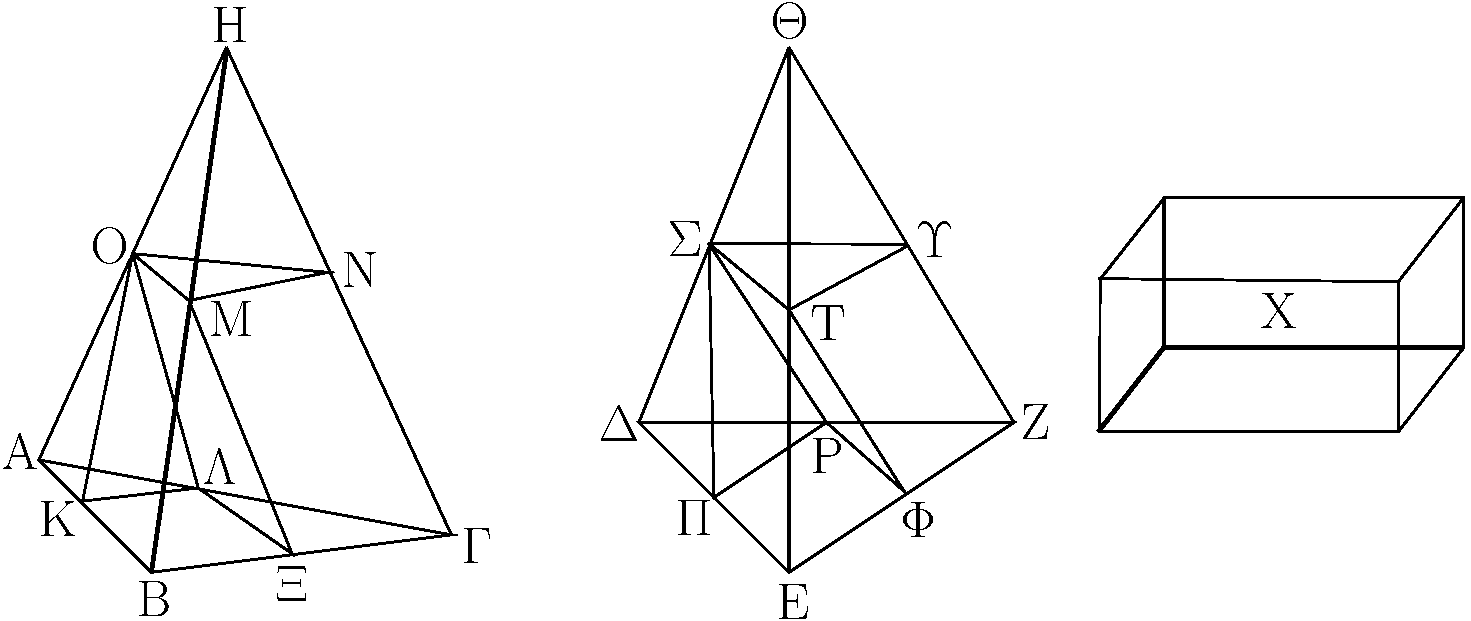
\includegraphics{Book12/fig05g.pdf}}

\gr{>'Εστωσαν ὑπὸ τὸ α\kern -.7pt  ὐτὸ <ύψοξ πυραμίδεξ, <ῶν βάσειξ μὲν τὰ ΑΒΓ, ΔΕΖ τρίγωνα, κορυφαὶ δὲ
τὰ Η, Θ σημεῖα; λέγω, <ότι ἐστὶν ὡξ ἡ ΑΒΓ βάσιξ πρὸξ τὴν ΔΕΖ βάσιν, ο<ύτωξ ἡ ΑΒΓΗ
πυραμὶξ πρὸξ τὴν ΔΕΖΘ πυραμίδα.}

\gr{Εἰ γὰρ μ\kern -.7pt  ή ἐστιν ὡξ ἡ ΑΒΓ βάσιξ πρὸξ τὴν ΔΕΖ βάσιν, ο<ύτωξ ἡ ΑΒΓΗ πυραμὶξ πρὸξ
τὴν ΔΕΖΘ πυραμίδα, >έσται ὡξ ἡ ΑΒΓ βάσιξ πρὸξ τὴν ΔΕΖ βάσιν, ο<ύτωξ ἡ ΑΒΓΗ πυραμὶξ
>ήτοι πρὸξ >έλασσόν τι τῆξ ΔΕΖΘ πυραμίδοξ στερεὸν >ὴ πρὸξ μεῖζον. >έστω πρότερον πρὸξ
>έλασσον τὸ Θ, καὶ διῃρὴσθω ἡ ΔΕΖΘ πυραμὶξ ε>ίξ τε δύο πυραμίδαξ >ίσαξ ἀλλήλαιξ καὶ
ὁμοίαξ τῆ| <όλῃ καὶ εἰξ δύο πρίσματα
>ίσα; τὰ δὴ δύο
πρίσαμτα μείζονά ἐστιν >ὴ τὸ <ήμισυ τῆξ <όληξ πυραμίδοξ. καὶ πάλιν αἱ ἐκ τῆξ διαιρέσεωξ
γινόμεναι πυραμίδεξ ὁμοίωξ διῃρήσθωσαν, καὶ τοῦτο ἀεὶ γινέσθω, <έωξ ο<ῦ λειφθῶσί
τινεξ πυραμίδεξ ἀπὸ τῆξ ΔΕΖΘ πυραμίδοξ, α<ί εἰσιν ἐλάττονεξ τῆξ ὑπεροθῆξ, <ῆ|
ὑπερέθει ἡ ΔΕΖΘ πυραμὶξ τοῦ Θ στερεοῦ. λελείφθωσαν καὶ >έστωσαν λόγου <ένεκεν
αἱ ΔΠΡΣ, ΣΤΥΘ; λοιπὰ >άρα τὰ ἐν τῆ| ΔΕΖΘ πυραμίδι πρίσματα μείζονά ἐστι τοῦ Θ στερεοῦ.
διῃρήσθω καὶ ἡ ΑΒΓΗ πυραμὶξ ὁμοίωξ καὶ ἰσοπληθῶξ τῆ| ΔΕΖΘ πυραμίδι;  >έστιν
>άρα ὡξ ἡ ΑΒΓ βάσιξ πρὸξ τὴν ΔΕΖ βάσιν, ο<ύτωξ τὰ ἐν τῆ| ΑΒΓΗ πυραμίδι πρίσματα
πρὸξ τὰ ἐν τῆ| ΔΕΖΘ πυραμίδι πρίσματα, ἀλλὰ καὶ ὡξ ἡ ΑΒΓ βάσιξ πρὸξ τὴν ΔΕΖ
βάσιν, ο<ύτωξ ἡ ΑΒΓΗ πυραμὶξ πρὸξ τὸ Θ στερεόν; καὶ ὡξ >άρα ἡ ΑΒΓΗ πυραμὶξ
πρὸξ τὸ Θ στερεόν, ο<ύτωξ τὰ ἐν τῆ| ΑΒΓΗ πυραμίδι πρίσματα πρὸξ τὰ ἐν τῆ| ΔΕΖΘ
πυραμίδι πρίσματα; ἐναλλὰχ >άρα ὡξ ἡ ΑΒΓΗ πυραμὶξ πρὸξ τὰ ἐν α\kern -.7pt  ὐτῆ| πρίσματα,
ο<ύτωξ τὸ Θ στερεὸν πρὸξ τὰ ἐν τῆ| ΔΕΖΘ πυραμίδι πρίσματα. μείζων δὲ ἡ ΑΒΓΗ πυραμὶξ
τῶν ἐν α\kern -.5pt  ὐτῆ| πρισμάτων; μεῖζον >άρα καὶ τὸ Θ στερεὸν τῶν ἐν τῆ| ΔΕΖΘ
πυραμίδι πρισμάτων. ἀλλὰ καὶ >έλαττον; <όπερ ἐστὶν ἀδύνατον. οὐκ >άρα ἐστὶν ὡξ ἡ ΑΒΓ
βάσιξ πρὸξ τὴν ΔΕΖ βάσιν, ο<ύτωξ ἡ ΑΒΓΗ πυραμὶξ πρὸξ >έλασσόν τι 
τῆξ ΔΕΖΘ
πυραμίδοξ στερεόν. ὁμοίωξ δὴ δειθθήσεται, <ότι οὐδὲ ὡξ ἡ ΔΕΖ βάσιξ πρὸξ τὴν
ΑΒΓ βάσιν, ο<ύτωξ ἡ ΔΕΖΘ πυραμὶξ πρὸξ >έλαττόν τι τῆξ ΑΒΓΗ πυραμίδοξ στερεόν.}

\gr{Λέγω δή, <ότι οὐκ >έστιν οὐδὲ ὡξ ἡ ΑΒΓ βάσιξ πρὸξ τὴν ΔΕΖ βάσιν, ο<ύτωξ ἡ
ΑΒΓΗ πυραμὶξ πρὸξ μεῖζόν τι τῆξ ΔΕΖΘ πυραμίδοξ στερεόν.}

\gr{Εἰ γὰρ δυνατόν, >έστω πρὸξ μεῖζον τὸ Θ; ἀνάπαλιν >άρα ἐστὶν ὡξ ἡ ΔΕΖ βάσιξ
πρὸξ τὴν ΑΒΓ βάσιν, ο<ύτωξ τὸ Θ στερεὸν πρὸξ τὴν ΑΒΓΗ πυραμίδα. ὡξ δὲ τὸ
Θ στερεὸν πρὸξ τὴν ΑΒΓΗ πυραμίδα, ο<ύτωξ ἡ ΔΕΖΘ πυραμὶξ πρὸξ >έλασσόν τι τῆξ
ΑΒΓΗ πυραμίδοξ, ὡξ >έμπροσθεν ἐδείθθη; καὶ ὡξ >άρα ἡ ΔΕΖ βάσιξ πρὸξ τὴν
ΑΒΓ βάσιν, ο<ύτωξ ἡ ΔΕΖΘ πυραμὶξ πρὸξ >έλασσόν τι τῆξ ΑΒΓΗ πυραμίδοξ; <όπερ
>άτοπον ἐδείθθη. οὐκ >άρα ἐστὶν ὡξ ἡ ΑΒΓ βάσιξ πρὸξ τὴν ΔΕΖ βάσιν, ο<ύτωξ
ἡ ΑΒΓΗ πυραμὶξ πρὸξ μεῖζόν τι τῆξ ΔΕΖΘ πυραμίδοξ στερεόν. ἐδείθθη δέ, <ότι
οὐδὲ πρὸξ >έλασσον. >έστιν >άρα ὡξ ἡ ΑΒΓ βάσιξ πρὸξ τὴν ΔΕΖ βάσιν,
ο<ύτωξ ἡ ΑΒΓΗ πυραμὶξ πρὸξ τὴν ΔΕΖΘ πυραμίδα; <όπερ >έδει δεῖχαι.}}

\ParallelRText{
\begin{center}
{\large Proposition 5}
\end{center}

Pyramids which are of the same height, and have triangular bases, are to one another
as their bases.

% Removed epsf size command
\centerline{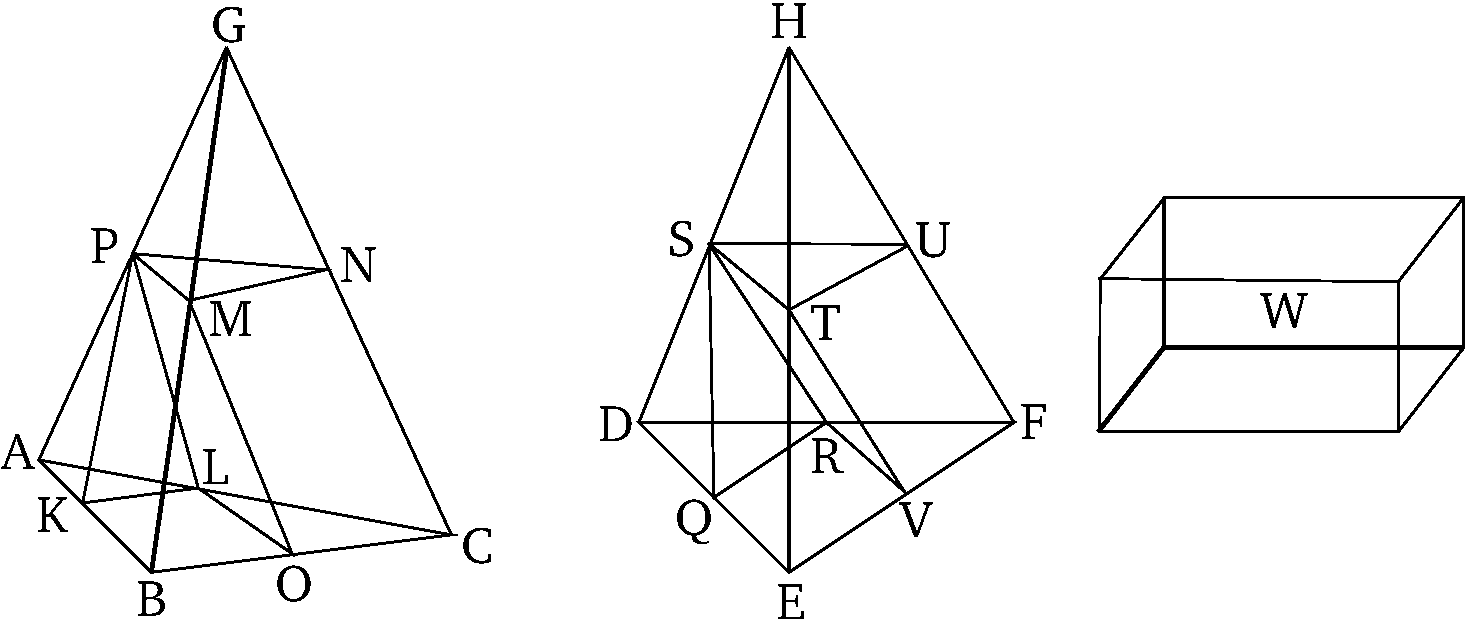
\includegraphics{Book12/fig05e.pdf}}

Let there be pyramids of the same height whose bases (are) the triangles $ABC$ and $DEF$, and apexes the
points $G$ and $H$ (respectively). I say that as base $ABC$ is to base $DEF$, so pyramid $ABCG$
(is) to pyramid $DEFH$.

For if base $ABC$ is not to base $DEF$, as pyramid $ABCG$ (is) to pyramid $DEFH$, then base
$ABC$ will be to base $DEF$, as pyramid $ABCG$ (is) to some solid either less than, or greater
than, pyramid $DEFH$. Let it, first of all, be (in this ratio) to (some) lesser (solid), $W$.
And let pyramid $DEFH$ be divided into two pyramids equal to one another, and
similar to the whole,  and into two equal prisms. So, the (sum of the) two prisms is greater than
half of the whole pyramid [Prop.~12.3].  And, again, let the pyramids generated
by the division be similarly divided, and let this be done continually until some pyramids
are left from pyramid $DEFH$ which (when added together) are less than the excess by which pyramid
$DEFH$ exceeds the solid $W$ [Prop.~10.1]. Let them be left, and, for the sake of argument, let them be $DQRS$ and $STUH$. Thus, the (sum of the) remaining prisms within pyramid $DEFH$ is greater than solid $W$. Let pyramid $ABCG$ also be divided similarly, and a similar number of times,
as pyramid $DEFH$. Thus, as base $ABC$ is to base $DEF$, so the (sum of the) prisms within pyramid $ABCG$
(is) to the (sum of the) prisms within pyramid $DEFH$ [Prop.~12.4]. But, also, as base
$ABC$ (is) to base $DEF$, so pyramid $ABCG$ (is) to solid $W$. And, thus, as pyramid $ABCG$ (is)
to solid $W$, so the (sum of the) prisms within pyramid $ABCG$ (is) to the (sum of the)
prisms within pyramid $DEFH$ [Prop.~5.11]. Thus, alternately, as pyramid $ABCG$ (is) to the (sum of the) prisms
within it, so solid $W$ (is) to the (sum of the) prisms within pyramid $DEFH$ [Prop.~5.16]. 
And  pyramid $ABCG$ (is) greater than the (sum of the) prisms within it. Thus, solid $W$ (is)
also greater than the (sum of the) prisms within pyramid $DEFH$ [Prop.~5.14]. But,
(it is) also less. This very thing is impossible. Thus, as base $ABC$ is to base $DEF$, so pyramid
$ABCG$ (is) not to some solid less than pyramid $DEFH$. So, similarly, we can show that 
base $DEF$ is not to base $ABC$, as pyramid $DEFH$ (is) to some solid less than pyramid $ABCG$ either.

So, I say that neither is base $ABC$ to base $DEF$, as pyramid $ABCG$ (is) to 
some solid greater
than pyramid $DEFH$.

For, if possible, let it be (in this ratio) to some greater (solid), $W$. Thus, inversely, as base $DEF$ (is) to base
$ABC$, so solid $W$ (is) to pyramid $ABCG$ [Prop.~5.7.~corr.]. And as solid $W$ (is) to pyramid $ABCG$, so pyramid
$DEFH$ (is) to some (solid) less than pyramid $ABCG$, as shown before [Prop.~12.2~lem.]. And, thus, as base $DEF$ (is) to base
$ABC$, so pyramid $DEFH$ (is) to some (solid) less than pyramid 
$ABCG$ [Prop.~5.11]. The very thing
was shown (to be) absurd. Thus, base $ABC$ is not to base $DEF$, as pyramid $ABCG$ (is) to some
solid greater than pyramid $DEFH$. And, it was shown that neither (is it in this ratio) to a lesser (solid). Thus, as base
$ABC$ is to base $DEF$, so pyramid $ABCG$ (is) to pyramid $DEFH$. (Which is) the very
thing it was required to show.}
\end{Parallel}

%%%%
%12.6
%%%%
\pdfbookmark[1]{Proposition 12.6}{pdf12.6}
\begin{Parallel}{}{}
\ParallelLText{
\begin{center}
{\large \ggn{6}.}
\end{center}\vspace*{-7pt}

\gr{Αἱ ὐπὸ τὸ α\kern -.7pt  ὐτὸ <ύψοξ ο>ῦσαι πυραμίδεξ καὶ πολυγώνουξ
>έθουσαι βάσειξ πρὸξ ἀλλήλαξ εἰσὶν ὡξ αἱ βάσειξ.}\\

% Removed epsf size command
\centerline{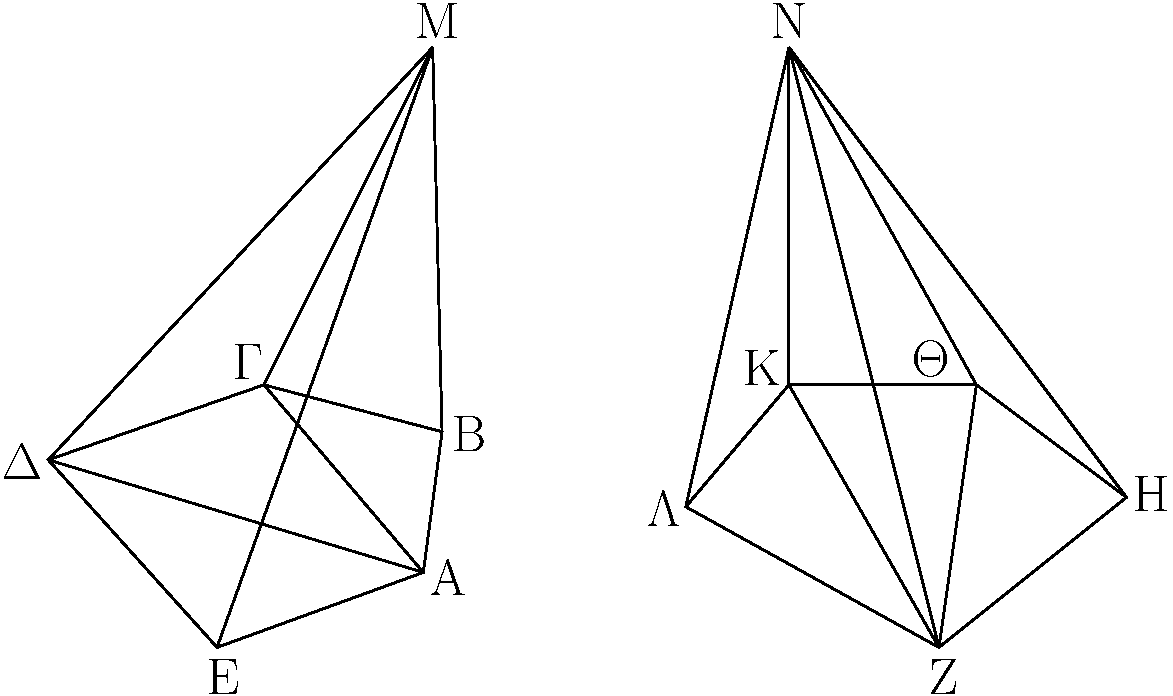
\includegraphics{Book12/fig06g.pdf}}

\gr{>'Εστωσαν ὑπὸ τὸ α\kern -.7pt  ὐτὸ <ύψοξ πυραμίδεξ, <ῶν [αἱ] βάσειξ
μὲν τὰ ΑΒΓΔΕ, ΖΗΘΚΛ πολύγωνα, κορυφαὶ δὲ τὰ Μ, Ν σημεῖα;
λέγω, <ότι ἐστὶν ὡξ ἡ ΑΒΓΔΕ βάσιξ πρὸξ τὴν ΖΗΘΚΛ βάσιν,
ο<ύτωξ ἡ ΑΒΓΔΕΜ πυραμὶξ πρὸξ τὴν ΖΗΘΚΛΝ πυραμίδα.}

\gr{Ἐπεζεύθθωσαν γὰρ αἱ ΑΓ, ΑΔ, ΖΘ, ΖΚ. ἐπεὶ ο>ῦν δύο πυραμίδεξ
εἰσὶν αἱ ΑΒΓΜ, ΑΓΔΜ τριγώνουξ >έθουσαι βάσειξ καὶ <ύψοξ
>ίσον, πρὸξ ἀλλήλαξ εἰσὶν ὡξ αἱ βάσειξ; >έστιν >άρα ὡξ ἡ ΑΒΓ βάσιξ πρὸξ τὴν ΑΓΔ βάσιν, ο<ύτωξ ἡ ΑΒΓΜ πυραμὶξ πρὸξ τὴν
ΑΓΔΜ πυραμίδα. καὶ συνθέντι ὡξ ἡ ΑΒΓΔ βάσιξ
πρὸξ τὴν ΑΓΔ βάσιν, ο<ύτωξ ἡ ΑΒΓΔΜ πυραμὶξ πρὸξ τὴν
ΑΓΔΜ πυραμίδα. ἀλλὰ καὶ ὡξ ἡ ΑΓΔ βάσιξ πρὸξ τὴν ΑΔΕ βάσιν,
ο<ύτωξ ἡ ΑΓΔΜ πυραμὶξ πρὸξ τὴν ΑΔΕΜ πυραμίδα. δι> >ίσου
>άρα ὡξ ἡ ΑΒΓΔ βάσιξ πρὸξ τὴν ΑΔΕ βάσιν, ο<ύτωξ ἡ
ΑΒΓΔΜ πυραμὶξ πρὸξ τὴν ΑΔΕΜ πυραμίδα. καὶ συνθέντι πάλιν,
ὡξ ἡ ΑΒΓΔΕ βάσιξ πρὸξ τὴν ΑΔΕ βάσιν, ο<ύτωξ ἡ ΑΒΓΔΕΜ 
πυραμὶξ πρὸξ τὴν ΑΔΕΜ πυραμίδα. ὁμοίωξ δὴ  δειθθήσεται,
<ότι καὶ ὡξ ἡ ΖΗΘΚΛ βάσιξ πρὸξ τὴν ΖΗΘ βάσιν, ο<ύτωξ
καὶ ἡ  ΖΗΘΚΛΝ πυραμὶξ πρὸξ τὴν ΖΗΘΝ πυραμίδα. καὶ ἐπεὶ
δύο πυραμίδεξ εἱσὶν αἱ ΑΔΕΜ, ΖΗΘΝ τριγώνουξ
>έθουσαι βάσειξ καὶ <ύψοξ >ίσον, >έστιν >άρα ὡξ ἡ ΑΔΕ
βάσιξ πρὸξ τὴν ΖΗΘ βάσιν, ο<ύτωξ ἡ ΑΔΕΜ πυραμὶξ πρὸξ
τὴν ΖΗΘΝ πυραμίδα. ἀλλ> ὡξ ἡ ΑΔΕ βάσιξ πρὸξ τὴν ΑΒΓΔΕ βάσιν,
ο<ύτωξ >ῆν ἡ ΑΔΕΜ πυραμὶξ πρὸξ τὴν ΑΒΓΔΕΜ πυραμίδα. καὶ δι> >ίσου >άρα ὡξ ἡ ΑΒΓΔΕ βάσιξ πρὸξ τὴν ΖΗΘ βάσιν, ο<ύτωξ
ἡ ΑΒΓΔΕΜ πυραμὶξ πρὸξ τὴν ΖΗΘΝ πυραμίδα. ἀλλὰ μ\kern -.7pt  ὴν καὶ
ὡξ ἡ ΖΗΘ βάσιξ πρὸξ τὴν ΖΗΘΚΛ βάσιν,
ο<ύτωξ >ῆν καὶ ἡ ΖΗΘΝ πυραμὶξ πρὸξ τὴν ΖΗΘΚΛΝ
πυραμίδα, καὶ δι> >ίσου >άρα ὡξ ἡ ΑΒΓΔΕ βάσιξ
πρὸξ τὴν ΖΗΘΚΛ βάσιν, ο<ύτωξ ἡ ΑΒΓΔΕΜ πυραμὶξ
πρὸξ τὴν ΖΗΘΚΛΝ πυραμίδα; <όπερ >έδει δεῖχαι.}}

\ParallelRText{
\begin{center}
{\large Proposition 6}
\end{center}

Pyramids which are of the same height, and have polygonal bases, are to one
another as their bases.\\

% Removed epsf size command
\centerline{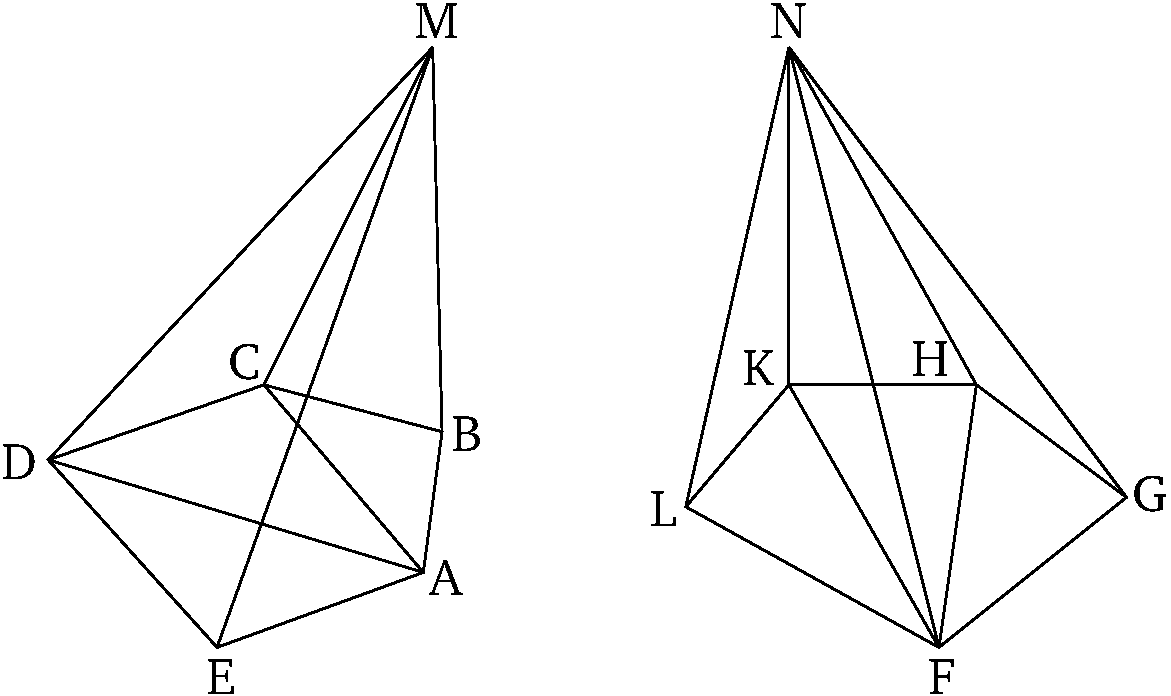
\includegraphics{Book12/fig06e.pdf}}

Let there be pyramids of the same height whose bases (are) the polygons $ABCDE$ and $FGHKL$,
and apexes the points $M$ and $N$ (respectively). I say that as base $ABCDE$ is to base $FGHKL$,
so pyramid $ABCDEM$ (is) to pyramid $FGHKLN$.

For let $AC$, $AD$, $FH$, and $FK$ be joined. Therefore, since $ABCM$ and
$ACDM$ are two pyramids having triangular bases and equal height, they are to one another
as their bases [Prop.~12.5]. Thus, as base $ABC$ is to base $ACD$, so pyramid 
$ABCM$ (is) to pyramid $ACDM$.  And, via composition, as base $ABCD$ (is) to base $ACD$, so
pyramid $ABCDM$ (is) to pyramid $ACDM$ [Prop.~5.18]. But, as base
$ACD$ (is) to base $ADE$, so pyramid $ACDM$ (is) also to pyramid $ADEM$ [Prop.~12.5]. Thus, via equality, 
as base $ABCD$ (is) to base $ADE$, so pyramid $ABCDM$ (is) to  pyramid $ADEM$ [Prop.~5.22]. And, again, via composition, as base $ABCDE$ (is) to base $ADE$,
so pyramid $ABCDEM$ (is) to pyramid $ADEM$ [Prop.~5.18]. 
So, similarly, it can also be shown that as base $FGHKL$ (is) to base $FGH$, so pyramid 
$FGHKLN$ (is) also to pyramid $FGHN$. And since $ADEM$ and $FGHN$ are two
pyramids having triangular bases and equal height,  thus as base $ADE$ (is) to base $FGH$, so
pyramid $ADEM$ (is) to pyramid $FGHN$ [Prop.~12.5]. 
But, as base $ADE$ (is) to base $ABCDE$,  so pyramid $ADEM$ (was) to 
pyramid $ABCDEM$. Thus, via equality,  as base $ABCDE$ (is) to base $FGH$,
so pyramid $ABCDEM$ (is) also to pyramid $FGHN$ [Prop.~5.22]. But,
furthermore, as base $FGH$ (is) to base $FGHKL$, so pyramid $FGHN$ was also to pyramid
$FGHKLN$. Thus, via equality, as base $ABCDE$ (is) to base $FGHKL$, so
pyramid $ABCDEM$ (is) also to pyramid $FGHKLN$  [Prop.~5.22]. (Which is) the very thing it was required
to show.}
\end{Parallel}

%%%%
%12.7
%%%%
\pdfbookmark[1]{Proposition 12.7}{pdf12.7}
\begin{Parallel}{}{}
\ParallelLText{
\begin{center}
{\large \ggn{7}.}
\end{center}\vspace*{-7pt}

\gr{Πᾶν πρίσμα τρίγωνον >έθον βάσιν διαιρεῖται εἰξ τρεῖξ πυραμίδαξ >ίσαξ ἀλλήλαιξ τριγώνουξ
βάσειξ ἐθούσαξ.}\\

% Removed epsf size command
\centerline{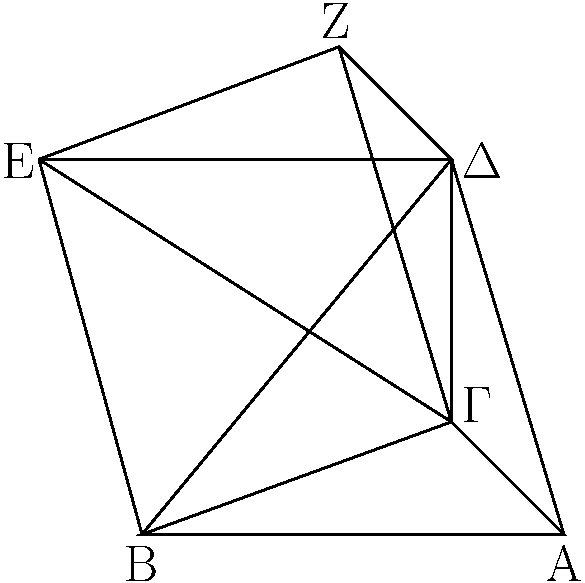
\includegraphics{Book12/fig07g.pdf}}

\gr{>'Εστω πρίσμα, ο<ῦ βάσιξ μὲν τὸ ΑΒΓ τρίγωνον, ἀπεναντίον δὲ τὸ ΔΕΖ; λέγω, <ότι
τὸ ΑΒΓΔΕΖ πρίσμα διαιρεῖται εἰξ τρεῖξ πυραμίδαξ >ίσαξ ἀλλήλαιξ τριγώνουξ ἐθούσαξ
βάσειξ.}

\gr{Ἐπεζεύθθωσαν γὰρ αἱ ΒΔ, ΕΓ, ΓΔ. ἐπεὶ παραλληλόγραμμόν ἐστι τὸ ΑΒΕΔ, διάμετροξ
δὲ α\kern -.7pt  ὐτὸῦ ἐστιν ἡ ΒΔ,  >ίσον >άρα ἐστι τὸ ΑΒΔ τρίγωνον τῶ| ΕΒΔ τρίγωνῳ; καὶ
ἡ πυραμὶξ >άρα, <ῆξ βάσιξ μὲν τὸ ΑΒΔ τρίγωνον, κορυφὴ δὲ τὸ Γ σημεῖον, >ίση ἐστὶ
πυραμίδι, <ῆξ βάσιξ μέν ἐστι τὸ ΔΕΒ τρίγωνον, κορυφὴ δὲ τὸ Γ σημεῖον. ἀλλὰ ἡ πυραμίξ,
<ῆξ βάσιξ μέν ἐστι τὸ ΔΕΒ τρίγωνον, κορυφὴ δὲ τὸ Γ σημεῖον, ἡ α\kern -.7pt  ὐτή ἐστι πυραμίδι,
<ῆξ βάσιξ μέν ἐστι τὸ ΕΒΓ τρίγωνον, κορυφὴ δὲ τὸ Δ σημεῖον; ὑπὸ γὰρ τῶν α\kern -.5pt  ὐτῶν
ἐπιπέδων περιέθεται. καὶ πυραμὶξ >άρα, <ῆξ βάσιξ μέν
ἐστι τὸ ΑΒΔ τρίγωνον, κορυφὴ δὲ τὸ Γ σημεῖον,
>ίση ἐστὶ πυραμίδι, <ῆξ βάσιξ μέν ἐστι τὸ ΕΒΓ τρίγωνον, κορυφὴ δὲ τὸ Δ σημεῖον. πάλιν,
ἐπεὶ παραλληλόγραμμόν ἐστι τὸ ΖΓΒΕ, διάμετροξ δέ ἐστιν α\kern -.3pt  ὐτοῦ ἡ ΓΕ, >ίσον ἐστὶ τὸ ΓΕΖ
τρίγωνον τῶ| ΓΒΕ τριγώνῳ. καὶ πυραμὶξ >άρα, <ῆξ βάσιξ μέν ἐστι τὸ ΒΓΕ τρίγωνον, κορυφὴ
δὲ τὸ Δ σημεῖον, >ίση ἐστὶ πυραμίδι, <ῆξ βάσιξ μέν ἐστι τὸ ΕΓΖ τρίγωνον, κορυφὴ
δὲ τὸ Δ σημεῖον. ἡ δὲ πυραμίξ, <ῆξ βάσιξ μέν ἐστι τὸ ΒΓΕ τρίγωνον, κορυφὴ δὲ τὸ
Δ σημεῖον, >ίση ἐδείθθη πυραμίδι, <ῆξ βάσιξ μέν ἐστι τὸ ΑΒΔ τρίγωνον, κορυφὴ δὲ τὸ
Γ σημεῖον; καὶ πυραμὶξ >άρα, <ῆξ βάσιξ μέν ἐστι τὸ ΓΕΖ τρίγωνον, κορυφὴ δὲ τὸ Δ
σημεῖον, >ίση ἐστὶ πυραμίδι, <ῆξ βάσιξ μέν [ἐστι] τὸ ΑΒΔ τρίγωνον, κορυφὴ δὲ τὸ
Γ σημεῖον; διή|ρηται >άρα τὸ ΑΒΓΔΕΖ πρίσμα εἰξ τρεῖξ πυραμίδαξ >ίσαξ ἀλλήλαιξ
τριγώνουξ ἐθούσαξ βάσειξ.}

\gr{Καὶ ἐπεὶ πυραμίξ, <ῆξ βάσιξ μέν ἐστι τὸ ΑΒΔ τρίγωνον, κορυφὴ δὲ τὸ Γ σημεῖον,
ἡ α\kern -.7pt  ὐτή ἐστι πυραμίδι, <ῆξ βάσιξ τὸ ΓΑΒ τρίγωνον, κορυφὴ δὲ τὸ Δ σημεῖον; ὑπὸ
γὰρ τῶν α\kern -.7pt  ὐτῶν ἐπιπέδων περιέθονται; ἡ δὲ πυραμίξ, <ῆξ βάσιξ τὸ ΑΒΔ τρίγωνον,
κορυφὴ δὲ τὸ Γ σημεῖον, τρίτον ἐδείθθη τοῦ πρίσματοξ, ο<ῦ βάσιξ τὸ ΑΒΓ τρίγωνον, ἀπεναντίον
δὲ τὸ ΔΕΖ, καὶ ἡ πυραμὶξ >άρα, <ῆξ βάσιξ τὸ ΑΒΓ τρίγωνον, κορυφὴ δὲ τὸ Δ σημεῖον,
τρίτον ἐστὶ τοῦ πρίσματοξ τοῦ >έθοντοξ βάσιξ τὴν α\kern -.5pt  ὐτὴν τὸ ΑΒΓ τρίγωνον, ἀπεναντίον
δὲ τὸ ΔΕΖ.}}

\ParallelRText{
\begin{center}
{\large Proposition 7}
\end{center}

Any prism having a triangular base is divided into three pyramids having triangular bases (which are) equal to
one another.

% Removed epsf size command
\centerline{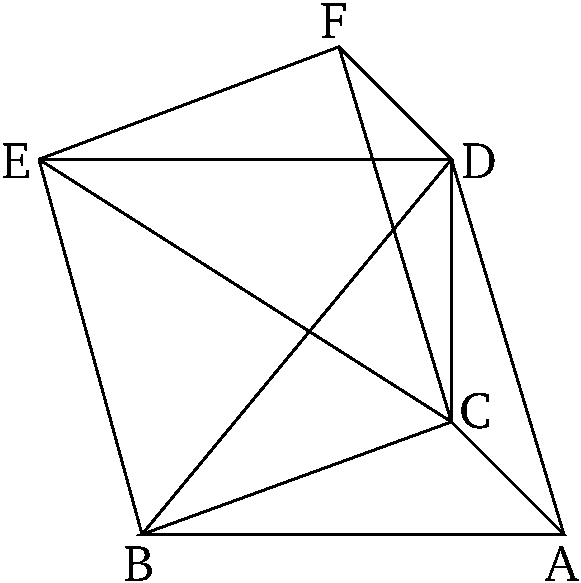
\includegraphics{Book12/fig07e.pdf}}

Let there be a prism whose base (is) triangle $ABC$, and opposite (plane) $DEF$. I say that
prism $ABCDEF$ is divided into three pyramids having
triangular bases (which are) equal to one another.

For let $BD$, $EC$, and $CD$ be joined. Since $ABED$ is a parallelogram, and $BD$ is its diagonal, triangle $ABD$ is thus equal to triangle $EBD$ [Prop.~1.34]. And, thus,
the pyramid whose base (is) triangle $ABD$, and apex the point $C$, is equal to the pyramid
whose base is triangle $DEB$, and apex the point $C$ [Prop.~12.5]. But,
the pyramid whose base is triangle $DEB$, and apex the point $C$, is the same as the pyramid whose
base is triangle $EBC$, and apex the point $D$. For they are contained
by the same planes. And, thus, the pyramid whose base is $ABD$, and
apex the point $C$, is equal to the pyramid whose base is $EBC$ and
apex the point $D$. 
Again, since $FCBE$ is a parallelogram, and
$CE$ is its diagonal, triangle $CEF$ is equal to triangle $CBE$ [Prop.~1.34].
And, thus, the pyramid whose base is triangle $BCE$, and apex the point $D$, is equal to the
pyramid whose base is triangle $ECF$, and apex the point $D$ [Prop.~12.5]. And the pyramid whose base
is triangle $BCE$, and apex the point $D$, was shown (to be) equal to the pyramid whose base is
triangle $ABD$, and apex the point $C$. Thus, the pyramid whose base is triangle $CEF$,
and apex the point $D$, is also equal to the pyramid whose base [is] triangle $ABD$, and apex
the point $C$. Thus, the prism $ABCDEF$ has been divided into three pyramids having triangular bases
(which are) equal to one another.

And since the pyramid whose base is triangle $ABD$, and apex the point $C$, is the
same as the pyramid whose base is triangle $CAB$, and apex the point $D$. For they are contained
by the same planes. And the pyramid whose base (is) triangle $ABD$, and apex the point
$C$, was shown (to be) a third of the prism whose base is triangle $ABC$, and opposite
(plane) $DEF$, thus the pyramid whose base is triangle $ABC$, and apex the point $D$, is  also
a third of the pyramid having the same base, triangle $ABC$, and opposite (plane)  $DEF$.}
\end{Parallel}

\begin{Parallel}{}{}
\ParallelLText{
\begin{center}
\large{\gr{Πόρισμα}.}
\end{center}\vspace*{-7pt}

\gr{Ἐκ δὴ τούτου φανερόν, <ότι πᾶσα πυραμὶξ τρίτον μέροξ ἐστὶ τοῦ πρίσματοξ τοῦ τὴν α\kern -.7pt  ὐτὴν
βάσιν >έθοντοξ α\kern -.7pt  ὐτῆ| καὶ <ύψοξ >ίσον; <όπερ >έδει δεῖχαι.}}

\ParallelRText{
\begin{center}
\large{Corollary}
\end{center}

And, from this, (it is) clear that any pyramid is the third part of the prism having the same
base as it, and an equal height. (Which is) the very thing it was required to show.}
\end{Parallel}

%%%%
%12.8
%%%%
\pdfbookmark[1]{Proposition 12.8}{pdf12.8}
\begin{Parallel}{}{}
\ParallelLText{
\begin{center}
{\large \ggn{8}.}
\end{center}\vspace*{-7pt}

\gr{Αἱ <όμοιαι πυραμίδεξ καὶ τριγώνουξ >έθουσαι βάσειξ ἐν τριπλασίονι λόγῳ εἰσὶ τῶν
ὁμολόγων πλευρῶν.}

\gr{>'Εστωσαν <όμοιαι καὶ ὁμοίωξ κείμεναι πυραμίδεξ, <ῶν βάσειξ μέν εἰσι τὰ
ΑΒΓ, ΔΕΖ τρίγωνα, κορυφαὶ δὲ τὰ Η, Θ σημεῖα; λέγω, <ότι ἡ ΑΒΓΗ πυραμὶξ
πρὸξ τὴν ΔΕΖΘ πυραμίδα τριπλασίονα λόγον >έθει >ήπερ ἡ ΒΓ πρὸξ τὴν ΕΖ.}

% Removed epsf size command
\centerline{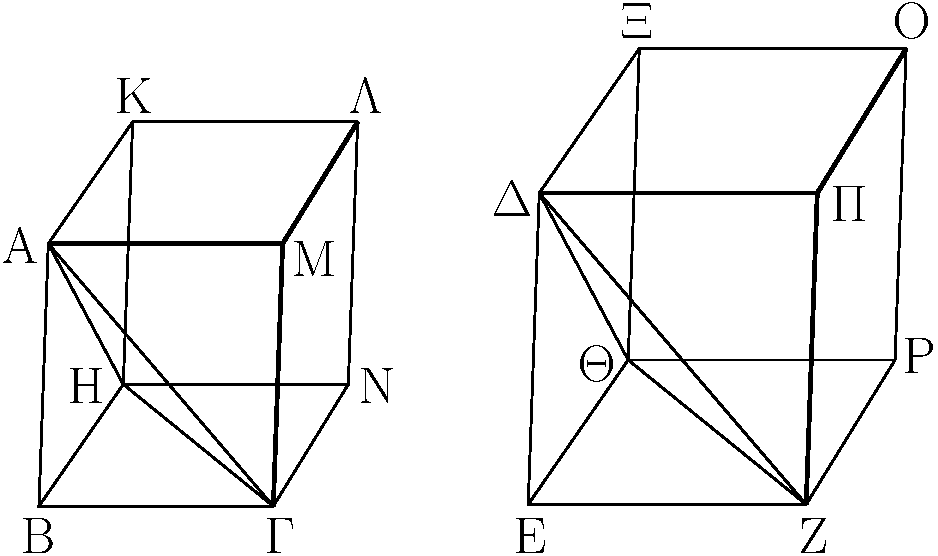
\includegraphics{Book12/fig08g.pdf}}

\gr{Συμπεπληρώσθω γὰρ τὰ ΒΗΜΛ, ΕΘΠΟ στερεὰ παραλληλεπίπεδα. καὶ ἐπεὶ ὁμοία
ἐστὶν ἡ ΑΒΓΗ πυραμὶξ τῆ| ΔΕΖΘ πυραμίδι, <ίση >άρα ἐστὶν ἡ μὲν ὑπὸ
ΑΒΓ γωνία τῆ| ὑπὸ ΔΕΖ γωνίᾳ, ἡ δὲ ὑπὸ ΗΒΓ τῆ| ὑπὸ ΘΕΖ, ἡ δὲ ὑπὸ
ΑΒΗ τῆ| ὑπὸ ΔΕΘ, καί ἐστιν ὡξ ἡ ΑΒ πρὸξ τὴν ΔΕ, ο<ύτωξ ἡ ΒΓ πρὸξ
τὴν ΕΖ, καὶ ἡ ΒΗ πρὸξ τὴν ΕΘ. 
καὶ ἐπεί ἐστιν ὡξ ἡ ΑΒ πρὸξ τὴν ΔΕ,
ο<ύτωξ ἡ ΒΓ πρὸξ τὴν ΕΖ, 
καὶ περὶ >ίσαξ γωνίαξ αἱ πλευραὶ ἀνάλογόν
εἰσιν, <όμοιον >άρα ἐστὶ τὸ ΒΜ παραλληλόγραμμον τῶ| ΕΠ παραλληλογράμμῳ.
διὰ τὰ α\kern -.7pt  ὐτὰ δὴ καὶ τὸ μὲν ΒΝ τῶ| ΕΡ <όμοιόν ἐστι, τὸ δὲ ΒΚ τῶ| ΕΧ; τὰ
τρία >άρα τὰ ΜΒ, ΒΚ, ΒΝ τρισὶ τοῖξ ΕΠ, ΕΧ, ΕΡ <όμοιά ἐστιν. 
ἀλλὰ τὰ μὲν τρία τὰ ΜΒ, ΒΚ, ΒΝ τρισὶ τοῖξ ἀπεναντίον >ίσα τε καὶ <όμοιά
ἐστιν, τὰ δὲ τρία τὰ ΕΠ, ΕΧ, ΕΡ τρισὶ τοῖξ ἀπεναντίον >ίσα τε καὶ <όμοιά ἐστιν.
τὰ ΒΗΜΛ, ΕΘΠΟ
>άρα στερεὰ ὑπὸ ὁμοίων ἐπιπέδων >ίσων τὸ πλῆθοξ περιέθεται. <όμοιον
>άρα ἐστὶ τὸ ΒΗΜΛ
στερεὸν τῶ| ΕΘΠΟ στερεῶ|. τὰ δὲ <όμοια στερεὰ παραλληλεπίπεδα ἐν τριπλασίονι λόγῳ
ἐστὶ τῶν ὁμολόγων πλευρῶν. τὸ ΒΗΜΛ >άρα στερεὸν πρὸξ τὸ ΕΘΠΟ στερεὸν
τριπλασίονα λόγον >έθει >ήπερ ἡ ὁμόλογοξ πλευρὰ ἡ ΒΓ πρὸξ τὴν ὁμόλογον
πλευρὰν τὴν ΕΖ. ὡξ δὲ τὸ ΒΗΜΛ στερεὸν πρὸξ τὸ ΕΘΠΟ στερεόν, ο<ύτωξ
ἡ ΑΒΓΗ πυραμὶξ πρὸξ τὴν ΔΕΖΘ πυραμίδα, ἐπειδήπερ ἡ πυραμὶξ <έκτον
μέροξ ἐστὶ τοῦ στερεοῦ διὰ τὸ καὶ τὸ πρίσμα <ήμισυ >ὸν τοῦ στερεοῦ
παραλληλεπιπέδου τριπλάσιον ε>ῖναι τῆξ πυραμίδοξ. καὶ ἡ ΑΒΓΗ >άρα 
πυραμὶξ πρὸξ
τὴν ΔΕΖΘ πυραμίδα τριπλασίονα λόγον >έθει  >ήπερ ἡ ΒΓ πρὸξ τὴν ΕΖ; <όπερ >έδει
δεῖχαι.}}

\ParallelRText{
\begin{center}
{\large Proposition 8}
\end{center}

Similar pyramids which also have triangular bases are in the cubed ratio of their
corresponding sides.

Let there be similar, and similarly laid out, pyramids whose bases are triangles $ABC$ and $DEF$, and apexes
the points $G$ and $H$ (respectively). I say that pyramid $ABCG$ has to pyramid $DEFH$ the cubed ratio
of that $BC$ (has) to $EF$. 

% Removed epsf size command
\centerline{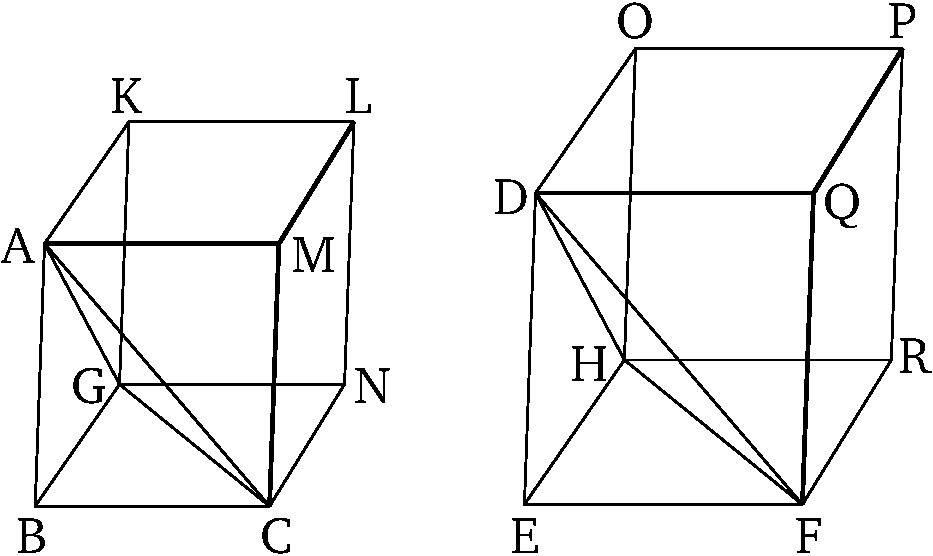
\includegraphics{Book12/fig08e.pdf}}

For let the parallelepiped solids $BGML$ and $EHQP$ be completed. And since pyramid $ABCG$
is similar to pyramid $DEFH$, angle $ABC$ is thus equal to angle $DEF$, and $GBC$ to $HEF$, and $ABG$
to $DEH$. And as $AB$ is to $DE$, so $BC$ (is) to $EF$, and $BG$ to $EH$ [Def.~11.9]. 
And since as $AB$ is to $DE$, so $BC$ (is) to $EF$, and (so) the sides around equal angles are proportional, parallelogram
$BM$ is thus similar to paralleleogram $EQ$. So, for the same (reasons), $BN$ is also similar to $ER$, and $BK$
to $EO$. Thus, the three (parallelograms) $MB$, $BK$, and $BN$ are similar to the three (parallelograms) $EQ$, $EO$,
$ER$ (respectively). But, the three (parallelograms) $MB$, $BK$, and $BN$ are (both) equal and similar to the three  opposite (parallelograms),
and the three (parallelograms) $EQ$, $EO$, and $ER$ are (both) equal and similar to the three opposite
 (parallelograms) [Prop.~11.24]. Thus, the solids $BGML$ and $EHQP$ are contained by
 equal numbers of similar (and similarly laid out) planes. Thus, solid $BGML$ is similar to solid $EHQP$ [Def.~11.9].
 And similar parallelepiped solids are in the cubed ratio of corresponding sides [Prop.~11.33].
 Thus, solid $BGML$ has to solid $EHQP$ the cubed ratio that the corresponding side $BC$ (has) to the corresponding
 side $EF$. And as solid $BGML$ (is) to solid $EHQP$, so pyramid $ABCG$ (is) to pyramid
 $DEFH$, inasmuch as the pyramid is the sixth part of the solid, on account of the prism, being half of the
 parallelepiped solid [Prop.~11.28], also being three times the pyramid [Prop.~12.7].
 Thus, pyramid $ABCG$ also has to pyramid $DEFH$ the cubed ratio that $BC$ (has) to $EF$. (Which is)
 the very thing it was required to show.}
 \end{Parallel}

\begin{Parallel}{}{}
\ParallelLText{
\begin{center}
\large{\gr{Πόρισμα}.}
\end{center}\vspace*{-7pt}

\gr{Ἐκ δὴ τούτου φανερόν, <ότι καὶ αἱ πολυγώνουξ >έθουσαι βάσειξ <όμοιαι πυραμίδεξ
πρὸξ ἀλλήλαξ ἐν τριπλασίονι λόγῳ εἰσὶ τῶν ὁμολόγων πλευρῶν.
διαιρεθεισῶν γὰρ α\kern -.7pt  ὐτῶν εἰξ τὰξ ἐν α\kern -.7pt  ὐταῖξ πυραμίδαξ τριγώνουξ βάσειξ
ἐθούσαξ τῶ| καὶ τὰ <όμοια πολύγωνα τῶν βάσεων εἰξ <όμοια τρίγωνα διαιρεῖσθαι
καὶ >ίσα τῶ| πλήθει καὶ ὁμόλογα τοῖξ <όλοιξ >έσται ὡξ [ἡ] ἐν τῆ| ἑτέρᾳ μία
πυραμὶξ τρίγωνον >έθουσα βάσιν πρὸξ τὴν ἐν τῆ| ἑτέρᾳ μίαν πυραμίδα τρίγωνον
>έθουσαν βάσιν, ο<ύτωξ καὶ <άπασαι αἱ ἐν τῆ| ἑτέρᾳ πυραμίδι πυραμίδεξ
τριγώνουξ >έθουσαι βάσειξ πρὸξ τὰξ ἐν τῆ| ἑτέρᾳ
πυραμίδι πυραμίδαξ τριγώνουξ βάσειξ ἐθούσαξ, τουτέστιν
α\kern -.5pt  ὐτὴ ἡ πολύγωνον βάσιν >έθουσα πυραμὶξ πρὸξ τὴν  πολύγωνον βάσιν >έθουσαν πυραμίδα. ἡ δὲ τρίγωνον βάσιν >έθουσα πυραμὶξ
πρὸξ τὴν τρίγωνον βάσιν >έθουσαν ἐν τριπλασίονι λόγῳ ἐστὶ τῶν ὁμολόγον πλευρῶν; καὶ ἡ πολύγωνον
>άρα βάσιν >έθουσα πρὸξ τὴν ὁμοίαν βάσιν >έθουσαν τριπλασίονα λόγον
>έθει >ήπερ ἡ πλευρὰ πρὸξ τὴν πλευράν.}}

\ParallelRText{
 \begin{center}
 \large{Corollary}
 \end{center}
 
 So, from this, (it is) also clear that similar pyramids  having polygonal bases (are) to one another as the cubed
 ratio of their corresponding sides. For, dividing them into  the pyramids (contained) within them which have triangular bases, with 
 the similar  polygons of the bases also being divided into similar triangles (which are) both equal in number, and corresponding,  to the wholes
 [Prop.~6.20].
 As  one pyramid having a triangular base in the former (pyramid having a polygonal base is)  to  one pyramid 
 having a triangular  base  in the latter (pyramid having a polygonal base),  so  (the sum of) all the pyramids having triangular bases in  the former pyramid will also
 be to (the sum of) all the pyramids having triangular bases in the latter  pyramid [Prop.~5.12]---that is to say, the (former) pyramid itself
 having  a polygonal base to the (latter) pyramid having a polygonal base. And a pyramid having a triangular base is to a (pyramid) having a triangular base in the cubed ratio of
 corresponding sides [Prop.~12.8]. Thus, a (pyramid) having a polygonal base also has to  to a (pyramid) having a similar base
 the
 cubed ratio of a (corresponding) side to a (corresponding) side.}
 \end{Parallel}
 
%%%%
%12.9
%%%%
\pdfbookmark[1]{Proposition 12.9}{pdf12.9}
\begin{Parallel}{}{}
\ParallelLText{
\begin{center}
{\large \ggn{9}.}
\end{center}\vspace*{-7pt}

\gr{Τῶν >ίσων πυραμίδων καὶ τριγώνουξ βάσειξ ἐθουσῶν ἀντιπεπόνθασιν αἱ βάσειξ τοῖξ <ύψεσιν; καὶ <ῶν πυραμίδων τριγώνουξ βάσειξ
ἐθουσῶν ἀντιπεπόνθασιν αἱ βάσειξ τοῖξ <ύψεσιν, >ίσαι
εἰσὶν ἐκεῖναι.}

% Removed epsf size command
\centerline{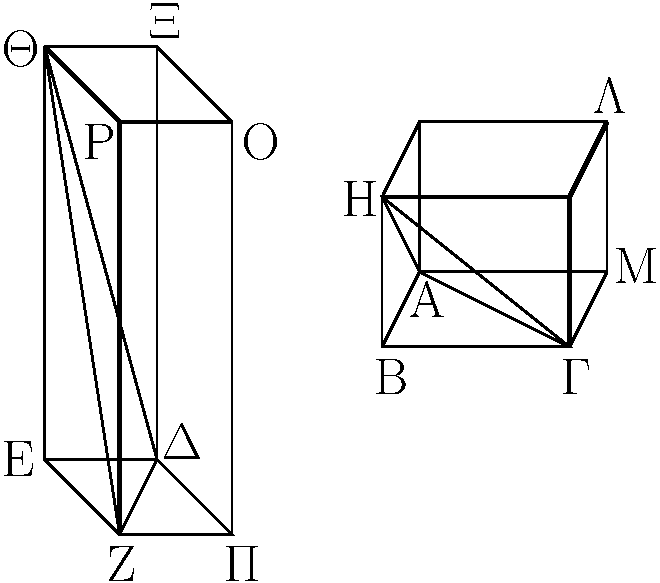
\includegraphics{Book12/fig09g.pdf}}

\gr{>'Εστωσαν γὰρ >ίσαι πυραμίδεξ τριγώνουξ βάσειξ >έθουσαι τὰξ ΑΒΓ,
ΔΕΖ, κορυφὰξ δὲ τὰ Η, Θ σημεῖα; λέγω, <ότι τῶν ΑΒΓΗ, ΔΕΖΘ
πυραμίδων ἀντιπεπόνθασιν αἱ βάσειξ τοῖξ <ύψεσιν, καί ἐστιν ὡξ ἡ
ΑΒΓ βάσιξ πρὸξ τὴν ΔΕΖ βάσιν, ο<ύτωξ τὸ τῆξ ΔΕΖΘ πυραμίδοξ
<ύψοξ πρὸξ τὸ τῆξ ΑΒΓΗ πυραμίδοξ <ύψοξ.}

\gr{Συμπεπληρώσθω γὰρ 		τὰ ΒΗΜΛ, ΕΘΠΟ στερεὰ παραλληλεπίπεδα. καὶ
ἐπεὶ >ίση ἐστὶν ἡ ΑΒΓΗ πυραμὶξ τῆ| ΔΕΖΘ πυραμίδι, καί ἐστι
τῆξ μὲν ΑΒΓΗ πυραμίδοξ ἑχαπλάσιον τὸ ΒΗΜΛ στερεόν, τῆξ
δὲ ΔΕΖΘ πυραμίδοξ ἑχαπλάσιον τὸ ΕΘΠΟ
στερεόν, >ίσον >άρα ἐστὶ τὸ ΒΗΜΛ στερεὸν τῶ| ΕΘΠΟ στερεῶ|.
τῶν δὲ >ίσων στερεῶν παραλληλεπιπώδων ἀντιπεπόνθασιν
αἱ βάσειξ τοῖξ <ύψεσιν; >έστιν >άρα ὡξ ἡ ΒΜ
βάσιξ πρὸξ τὴν ΕΠ βάσιν, ο<ύτωξ τὸ τοῦ ΕΘΠΟ στερεοῦ <ύψοξ
πρὸξ τὸ τοῦ ΒΗΜΛ στερεοῦ <ύψοξ. ἀλλ> ὡξ ἡ ΒΜ βάσιξ
πρὸξ τὴν ΕΠ, ο<ύτωξ τὸ ΑΒΓ τρίγωνον πρὸξ τὸ ΔΕΖ
τρίγωνον.
καὶ ὡξ >άρα τὸ ΑΒΓ τρίγωνον πρὸξ τὸ ΔΕΖ τρίγωνον,
 ο<ύτωξ τὸ τοῦ ΕΘΠΟ στερεοῦ <ύψοξ πρὸξ τὸ τοῦ
ΒΗΜΛ στερεοῦ <ύψοξ. ἀλλὰ τὸ μὲν τοῦ ΕΘΠΟ στερεοῦ
<ύψοξ τὸ α\kern -.7pt  ὐτὸ ἐστι τῶ| τῆξ ΔΕΖΘ πυραμίδοξ <ύψει,
τὸ δὲ τοῦ ΒΗΜΛ στερεοῦ <ύψοξ τὸ α\kern -.7pt  ὐτό ἐστι τῶ| τῆξ
ΑΒΓΗ πυραμίδοξ <ύψει; >έστιν >άρα ὡξ ἡ ΑΒΓ βάσιξ πρὸξ τὴν
ΔΕΖ βάσιν, ο<ύτωξ τὸ τῆξ ΔΕΖΘ πυραμίδοξ <ύψοξ πρὸξ τὸ τῆξ
ΑΒΓΗ πυραμίδοξ <ύψοξ. τῶν ΑΒΓΗ, ΔΕΖΘ >άρα πυραμίδων
ἀντιπεπόνθασιν αἱ βάσειξ τοῖξ <ύψεσιν.}

\gr{Ἀλλὰ δὴ τῶν ΑΒΓΗ, ΔΕΖΘ πυραμίδων ἀντιπεπονθέτ\-ωσαν
αἱ βάσειξ τοῖξ <ύψεσιν, καὶ >έστω ὡξ ἡ ΑΒΓ βάσιξ πρὸξ
τὴν ΔΕΖ βάσιν, ο<ύτωξ τὸ τῆξ ΔΕΖΘ πυραμίδοξ <ύψοξ
πρὸξ τὸ τῆξ ΑΒΓΗ πυραμίδοξ <ύψοξ; λέγω, <ότι >ίση ἐστὶν
ἡ ΑΒΓΗ πυραμὶξ τῆ| ΔΕΖΘ πυραμίδι.}

\gr{Τῶν γὰρ α\kern -.7pt  ὐτῶν κατασκευασθέντων, ἐπεί ἐστιν ὡξ ἡ ΑΒΓ βάσιξ
πρὸξ τὴν ΔΕΖ βάσιν, ο<ύτωξ τὸ τῆξ ΔΕΖΘ πυραμίδοξ <ύψοξ
πρὸξ τὸ τῆξ ΑΒΓΗ πυραμίδοξ <ύψοξ, ἀλλ> ὡξ ἡ ΑΒΓ
βάσιξ πρὸξ τὴν ΔΕΖ βάσιν, ο<ύτωξ τὸ ΒΜ παραλληλόγραμμον
πρὸξ τὸ ΕΠ παραλληλόγραμμον, καὶ ὡξ >άρα τὸ ΒΜ παραλληλόγραμμον
πρὸξ  τὸ ΕΠ παραλληλόγραμμον, ο<ύτωξ τὸ τῆξ ΔΕΖΘ πυραμίδοξ
<ύψοξ πρὸξ τὸ τῆξ ΑΒΓΗ πυραμίδοξ
<ύψοξ. ἀλλὰ τὸ [μὲν] τῆξ ΔΕΖΘ πυραμίδοξ <ύψοξ τὸ α\kern -.7pt  ὐτό ἐστι
τῶ| τοῦ ΕΘΠΟ παραλληλεπιπέδου
<ύψει, τὸ δὲ τῆξ ΑΒΓΗ πυραμίδοξ <ύψοξ τὸ α\kern -.5pt  ὐτό
ἐστι τῶ| τοῦ ΒΗΜΛ παραλληλεπιπέδου <ύψει;  >έστιν >άρα ὡξ ἡ ΒΜ
βάσιξ πρὸξ τὴν ΕΠ βάσιν, ο<ύτωξ τὸ τοῦ ΕΘΠΟ παραλληλεπιπέδου
<ύψοξ πρὸξ τὸ τοῦ ΒΗΜΛ παραλληλεπιπέδου <ύψοξ. <ῶν δὲ
στερεῶν παραλληλεπιπέδων ἀντιπεπόνθασιν αἱ βάσειξ τοῖξ
<ύψεσιν, >ίσα ἐστὶν ἐκεῖνα; >ίσον >άρα ἐστὶ τὸ ΒΗΜΛ
στερεὸν παραλληλεπίπεδον  τῶ| ΕΘΠΟ στερεῶ| παραλληλεπιπέδῳ.
καί ἐστι τοῦ μὲν ΒΗΜΛ <έκτον μέροξ ἡ ΑΒΓΗ
πυραμίξ, τοῦ δὲ ΕΘΠΟ παραλληλεπιπέδου <έκτον μέροξ ἡ ΔΕΖΘ πυραμίξ;
>ίση >άρα ἡ ΑΒΓΗ πυραμὶξ τῆ| ΔΕΖΘ πυραμίδι.}

\gr{Τῶν >άρα >ίσων πυραμίδων καὶ τριγώνουξ βάσειξ ἐθουσῶν
ἀντιπεπόνθασιν αἱ βάσειξ τοῖξ <ύψεσιν; καὶ <ῶν πυραμίδων τριγώνουξ βάσειξ
ἐθουσῶν ἀντιπεπόνθασιν αἱ
βάσειξ τοῖξ <ύψεσιν, >ίσαι εἰσὶν ἐκεῖναι; <όπερ 
>έδει δεῖχαι.}}

\ParallelRText{
\begin{center}
{\large Proposition 9}
\end{center}

The bases of equal pyramids which also have triangular bases are reciprocally
proportional to their heights. And those pyramids which have triangular bases whose bases are reciprocally
proportional to their heights  are equal.

% Removed epsf size command
\centerline{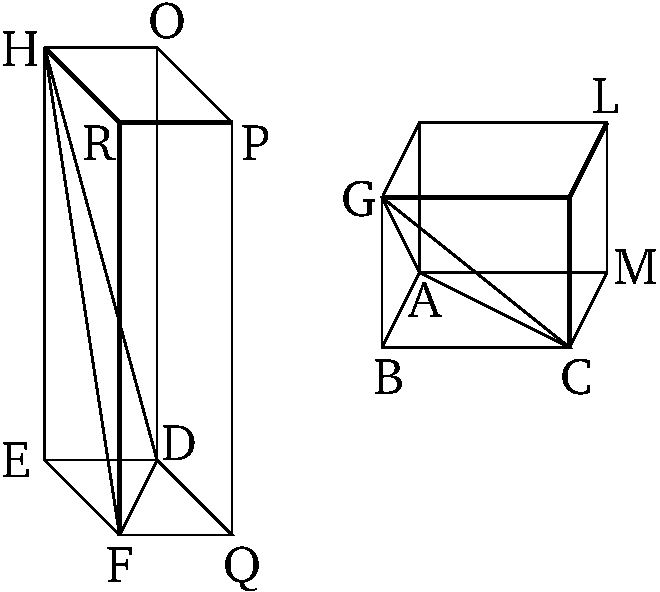
\includegraphics{Book12/fig09e.pdf}}

For let there be (two) equal pyramids having the triangular bases $ABC$ and $DEF$, and apexes
the points $G$ and $H$ (respectively). I say that the bases of the pyramids $ABCG$ and
$DEFH$ are reciprocally proportional to their heights, and (so) that as base $ABC$ is to base
$DEF$, so the height of pyramid $DEFH$ (is) to the height of pyramid $ABCG$.

For let the parallelepiped solids $BGML$ and $EHQP$ be completed. And since pyramid
$ABCG$ is equal to pyramid $DEFH$, and solid $BGML$ is six times pyramid $ABCG$ (see previous
proposition), and solid $EHQP$ (is) six times pyramid $DEFH$, solid $BGML$ is thus equal to
solid $EHQP$. And the bases of equal parallelepiped solids are reciprocally proportional
to their heights [Prop.~11.34]. Thus, as base $BM$ is to base $EQ$, so the height of
solid $EHQP$ (is) to the height of solid $BGML$. But, as base $BM$ (is) to base $EQ$, so triangle
$ABC$ (is) to triangle $DEF$ [Prop.~1.34]. And, thus, as triangle $ABC$ (is) to triangle
$DEF$, so the height of solid $EHQP$ (is) to the height of solid $BGML$ [Prop.~5.11]. But, the height of
solid $EHQP$ is the same as the height of pyramid $DEFH$, and the height of solid $BGML$ is the
same as the height of pyramid $ABCG$. Thus, as base $ABC$ is to base $DEF$, so the
height of pyramid $DEFH$ (is) to the height of pyramid $ABCG$. Thus, the bases of pyramids
$ABCG$ and $DEFH$ are reciprocally proportional to their heights.

And so, let the bases of pyramids $ABCG$ and $DEFH$ be reciprocally proportional to their heights, and (thus) let
base $ABC$ be to base $DEF$, as the height of pyramid $DEFH$ (is) to the height of pyramid $ABCG$.
I say that pyramid $ABCG$ is equal to pyramid $DEFH$.

For, with the same construction, since as base $ABC$ is to base $DEF$, so the height of pyramid $DEFH$ (is)
to the height of pyramid $ABCG$, but as base $ABC$ (is) to base $DEF$, so parallelogram $BM$ (is)
to parallelogram $EQ$ [Prop.~1.34], thus as parallelogram $BM$ (is) to
parallelogram $EQ$, so the height of pyramid $DEFH$  (is) also to the height of pyramid $ABCG$ [Prop.~5.11]. But, 
the height of pyramid $DEFH$ is the same as the height of parallelepiped $EHQP$, and the height of
pyramid $ABCG$ is the same as the height of parallelepiped $BGML$. Thus, as base $BM$ is to
base $EQ$, so the height of parallelepiped $EHQP$ (is) to the height of parallelepiped $BGML$.
And those parallelepiped solids whose bases are reciprocally proportional to their
heights are equal [Prop.~11.34]. Thus, the parallelepiped solid $BGML$ is equal to the parallelepiped
solid $EHQP$. And pyramid $ABCG$ is a sixth part of $BGML$, and pyramid $DEFH$ a sixth part of
parallelepiped $EHQP$. Thus, pyramid $ABCG$ is equal to pyramid $DEFH$.

Thus,  the bases of equal pyramids which also have triangular bases are reciprocally
proportional to their heights. And those pyramids having triangular bases whose bases are reciprocally
proportional to their heights  are equal. (Which is) the very thing it was required to show.}
\end{Parallel}

%%%%
%12.10
%%%%
\pdfbookmark[1]{Proposition 12.10}{pdf12.10}
\begin{Parallel}{}{}
\ParallelLText{
\begin{center}
{\large \ggn{10}.}
\end{center}\vspace*{-7pt}

\gr{Πᾶξ κῶνοξ κυλίνδρου τρίτον μέροξ ἐστὶ τοῦ τὴν α\kern -.7pt  ὐτὴν βάσιν >έθοντοξ α\kern -.7pt  ὐτῶ| καὶ <ύψοξ >ίσον.}

\gr{Ἐθέτω γὰρ κῶνοξ κυλίνδρῶ| βάσιν τε τὴν α\kern -.7pt  ὐτὴν τὸν ΑΒΓΔ κύκλον καὶ <ύψοξ >ίσον; λέγω, <ότι
ὁ κῶνοξ τοῦ κυλίνδρου τρίτον ἐστὶ μέροξ, τουτέστιν <ότι ὁ κύλινδροξ τοῦ κώνου τριπλασίων
ἐστίν.}

% Removed epsf size command
\centerline{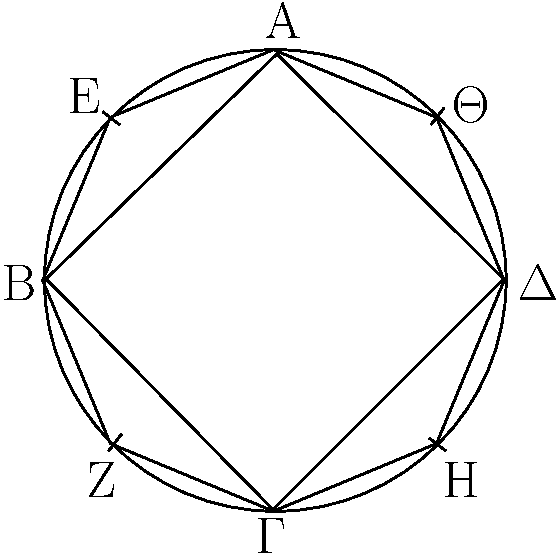
\includegraphics{Book12/fig10g.pdf}}

\gr{Εἰ γὰρ μ\kern -.7pt  ή ἐστιν ὁ κύλινδροξ τοῦ κώνου τριπλασίων, >έσται ὁ κύλινδροξ τοῦ κώνου >ήτοι μείζων
>ὴ τριπλασίων >ὴ  ἐλάσσων >ὴ τριπλασίων. >έστω πρότερον μείζων >ὴ τριπλασίων, καὶ ἐγγεγράφθω εἰξ
τὸν ΑΒΓΔ κύκλον τετράγων\-ον τὸ ΑΒΓΔ; τὸ δὴ ΑΒΓΔ τετράγωνον μείζόν ἐστιν >ὴ τὸ <ήμισυ
τοῦ ΑΒΓΔ κύκλου. καὶ ἀνεστάτω ἀπὸ τοῦ ΑΒΓΔ τετραγώνου πρίσμα 
ἰσο"υψὲξ τῶ| κυλίνδρῳ.
τὸ δὴ ἀνιστάμενον πρίσμα μεῖζόν ἐστιν >ὴ τὸ <ήμισυ τοῦ κυλίνδου, ἐπειδήπερ κ>ὰν περὶ
τὸν ΑΒΓΔ κύκλον τετράγωνον περιγράψωμεν, τὸ ἐγγεγραμμένον εἰξ τὸν ΑΒΓΔ κύκλον τετράγωνον
<ήμισύ ἐστι τοῦ περιγεγραμμένου; καί ἐστι τὰ ἀπ> α\kern -.7pt  ὐτῶν ἀνιστάμενα στερεὰ παραλληλεπίπεδα πρίσματα
ἰσο"υψῆ; τὰ δὲ ὑπὸ τὸ α\kern -.5pt  ὐτὸ <ύψοξ >όντα στερεὰ παραλληλεπίπεδα πρὸξ >άλληλά ἐστιν ὡξ αἱ βάσειξ;
καὶ τὸ ἐπὶ τοῦ ΑΒΓΔ >άρα τετραγώνου ἀνασταθὲν πρίσμα <ήμισύ ἐστι τοῦ ἀνασταθέντοξ πρίσματοξ
ἀπὸ τοῦ περὶ τὸν ΑΒΓΔ κύκλον περιγραφέντοξ τετραγώνου; καί ἐστιν ὁ κύλινδροξ ἐλάττων τοῦ
πρίσματοξ τοῦ ἀνατραθέντοξ ἀπὸ τοῦ περὶ τὸν ΑΒΓΔ κύκλον περιγραφέντοξ τετραγώνου;
τὸ >άρα πρίσμα τὸ ἀνασταθὲν ἀπὸ τοῦ ΑΒΓΔ τετραγώνου ἰσο"υψὲξ τῶ| κυλίνδρῳ μεῖζόν ἐστι τοῦ
ἡμίσεωξ τοῦ κυλίνδρου. τετμ\kern -.3pt  ήσθωσαν αἱ ΑΒ, ΒΓ, ΓΔ, ΔΑ περιφέρειαι δίθα κατὰ τὰ Ε, Ζ, Η, Θ σημεῖα,
καὶ ἐπεζεύθθωσαν αἱ ΑΕ, ΕΒ, ΒΖ, ΖΓ, ΓΗ, ΗΔ, ΔΘ, ΘΑ; καὶ <έκαστον >άρα τῶν ΑΕΒ, ΒΖΓ, ΓΗΔ, ΔΘΑ
τριγώνων μειζόν ἐστιν >ὴ τὸ <ήμισυ τοῦ καθ> ἑαυτὸ τηήματοξ τοῦ ΑΒΓΔ κύκλου, ὡξ >έμπροσθεν
ἐδείκνυμεν. ἀνεστάτω ἐφ> ἑκάστου τῶν ΑΕΒ, ΒΖΓ, ΓΗΔ, ΔΘΑ τριγώνων πρίσματα
ἰσο"υψῆ τῶ| κυλίνδρῳ; καὶ <έκαστον >άρα τῶν ἀνασταθέντων πρισμάτων μεῖζόν ἐστιν >ὴ τὸ
<ήμισυ μέροξ τοῦ καθ> ἑαυτὸ τμ\kern -.7pt  ήματοξ τοῦ κυλίνδρου, ἐπειδήπερ ἒαν διὰ τῶν Ε, Ζ, Η, Θ
σημείων παραλλήλουξ ταῖξ ΑΒ, ΒΓ, ΓΔ, ΔΑ ἀγάγωμεν, καὶ 
συμπληρώσωμεν τὰ ἐπὶ τῶν ΑΒ, 
ΒΓ, ΓΔ, ΔΑ παραλληλόγραμμα, καὶ  ἀπ> α\kern -.7pt  ὐτῶν ἀναστήσωμεν στερεὰ  παραλληλεπίπεδα ἰσο"υψῆ
τῶ| κυλίνδρῳ, ἑκάσου τῶν ἀνασταθέντων ἡμίση ἐστὶ τὰ πρίσματα τὰ ἐπὶ τῶν
ΑΕΒ, ΒΖΓ, ΓΗΔ, ΔΘΑ τριγώνων;  καί ἐστι τὰ τοῦ κυλίνδρου τμ\kern -.7pt  ήματα ἐλάττονα τῶν ἀνασταθέντων
στερεῶν παραλληλεπιπέδων; <ώστε καὶ τὰ ἐπὶ τῶν ΑΕΒ, ΒΖΓ, ΓΗΔ, ΔΘΑ τριγώνων πρίσματα μείζονά
ἐστιν >ὴ τὸ <ήμισυ τῶν καθ> ἑαυτὰ τοῦ κυλίνδρου τμ\kern -.7pt  ημάτων. τέμνοντεξ δὴ τὰξ ὑπολειπομέναξ περιφερείαξ
δίθα καὶ ἐπιζευγνύντεξ εὐθείαξ καὶ ἀνιστάντεξ 
ἐφ> ἑκάσου τῶν τριγώνων πρίσματα ἰσο"υψῆ τῶ| κυλίνδρῳ καὶ τοῦτο ἀεὶ ποιοῦντεξ καταλείψομέν
τινα ἀποτμ\kern -.7pt  ήματα τοῦ κυλίνδρου, <ὰ >έσται ἐλάττονα τῆξ ὑπεροθῆξ, <ῆ| ὑπερέθει ὁ κυλίνδροξ τοῦ
τριπλασίου τοῦ κώνου. λελείφθω, καὶ >έστω τὰ ΑΕ, ΕΒ, ΒΖ, ΖΓ, ΓΗ, ΗΔ, ΔΘ, ΘΑ; λοιπὸν >άρα τὸ πρίσμα, ο<ῦ
βάσιξ μὲν τὸ ΑΕΒΖΓΗΔΘ πολύγωνον, <ύψοξ δὲ τὸ α\kern -.7pt  ὐτὸ τῶ| κυλίνδρῶ|, μεῖζόν ἐστὶν >ὴ
τριπλάσιον τοῦ κώνου. 
ἀλλὰ τὸ πρίσμα, ο<ῦ βάσιξ μὲν ἐστὶ τὸ ΑΕΒΖΓΗΔΘ πολύγωνον, <ύψοξ δὲ τὸ α\kern -.7pt  ὐτὸ τῶ| κυλίνδρῳ, τριπλάσιόν
ἐστι τῆξ πυραμίδοξ, <ῆξ βάσιξ μέν ἐστι τὸ ΑΕΒΖΓΗΔΘ
πολύγωνον, 
κορυφὴ δὲ
ἡ α\kern -.7pt  ὐτὴ τῶ| κώνῳ; καὶ ἡ πυραμὶξ >άρα, <ῆξ βάσιξ μέν [ἐστι] τὸ ΑΕΒΖΓΗΔΘ πολύγωνον, κορυφὴ
δὲ ἡ α\kern -.7pt  ὐτὴ τῶ| κώνῳ, μείζων ἐστὶ τοῦ κώνου τοῦ βάσιν >έθοντεξ τὸν ΑΒΓΔ κύκλον.
 ἀλλὰ καὶ
ἐλάττων; ἐμπεριέθεται γὰρ ὑπ> α\kern -.7pt  ὐτοῦ; <όπερ ἐστὶν ἀδύνατον. οὐκ >άρα ἐστὶν ὁ κύλινδροξ
τοῦ κώνου μεῖζων >ὴ τριπλάσιοξ.}

\gr{Λέγω δή,  <ότι οὐδὲ ἐλάττων ἐστὶν >ὴ τριπλάσιοξ ὁ κύλινδροξ τοῦ κώνου.}

\gr{Εἰ γὰρ δυνατόν, >έστω ἐλάττων >ὴ τριπλάσιοξ ὁ κύλινδροξ τοῦ κώνου;
  ἀνάπαλιν >άρα ὁ κῶνοξ
τοῦ κυλίνδρου μεῖζων ἐστὶν >ὴ τρίτον μέροξ. ἐγγεγράφθω δὴ εἰξ τὸν ΑΒΓΔ κύκλον τετράγωνον τὸ
ΑΒΓΔ; τὸ ΑΒΓΔ >άρα τετράγωνον μεῖζόν ἐστιν >ὴ τὸ <ήμισυ τοῦ ΑΒΓΔ κύκλου. καὶ ἀνεστάτω
ἀπὸ τοῦ ΑΒΓΔ τετραγώνου πυραμὶξ τὴν α\kern -.7pt  ὐτὴν κορυφὴν >έθουσα τῶ| κώνῳ; ἠ >άρα ἀνασταθεῖσα
πυραμὶξ μείζων ἐστὶν >ὴ τὸ <ήμισυ μέροξ τοῦ κώνου, ἐπειδήπερ, ὡξ <έμπροσθεν ἐδείκνυμεν,
<ότι ἒαν περὶ τὸν κύκλον τετράγωνον περιγράψωμεν, >έσται τὸ ΑΒΓΔ τετράγωνον <ήμισυ τοῦ
περὶ τὸν κύκλον περιγεγραμμένου τετραγώνου; καὶ ἒαν ἀπὸ τῶν τετραγώνων στερεὰ παραλληλεπίπεδα
ἀναστήσωμεν ἰσο"υψῆ τῶ| κώνῳ, >ὰ καὶ καλεῖται πρίσματα, >έσται τὸ ἀνασταθὲν ἀπὸ τοῦ
ΑΒΓΔ τετραγώνου <ήμισυ τοῦ ἀνασταθέντοξ ἀπὸ τοῦ περὶ τὸν κύκλον περιγραφέντοξ τετραγώνου;
πρὸξ >άλληλα γάρ εἰσιν ὡξ αἱ βάσειξ. <ώστε καὶ τὰ τρίτα; καὶ πυραμὶξ >άρα, <ῆξ βάσιξ
τὸ ΑΒΓΔ τετράγωνον, <ήμισύ ἐστι τῆξ πυραμίδοξ τῆξ ἀνασταθείσηξ ἀπὸ τοῦ περὶ τὸν
κύκλον περιγραφέντοξ τετραγώνου.
καί ἐστι μείζων ἡ πυραμὶξ ἡ ἀνασταθεῖσα ἀπὸ τοῦ περὶ τὸν κύκλον τετραγώνου τοῦ κώνου;
ἐμπεριέθει γὰρ α\kern -.7pt  ὐτόν. ἡ >άρα πυραμὶξ, <ῆξ βάσιξ τὸ ΑΒΓΔ τετράγωνον, κορυφὴ δὲ ἡ α\kern -.5pt  ὐτὴ
τῶ| κώνῳ, μείζων ἐστὶν >ὴ τὸ <ήμισυ τοῦ κώνου. τετμ\kern -.3pt  ήσθωσαν αἱ ΑΒ, ΒΓ, ΓΔ, ΔΑ περιφέρειαι
δίθα κατὰ τὰ Ε, Ζ, Η, Θ σημεῖα, καὶ ἐπεζεύθθωσαν αἱ ΑΕ, ΕΒ, ΒΖ, ΖΓ, ΓΗ, ΗΔ, ΔΘ, ΘΑ; καὶ <έκαστον
>άρα τῶν ΑΕΒ, ΒΖΓ, ΓΗΔ, ΔΘΑ τριγώνων μεῖζόν ἐστιν >ὴ τὸ <ήμισυ μέροξ του καθ>
ἑαυτὸ τμ\kern -.7pt  ήματοξ  τοῦ ΑΒΓΔ κύκλου.
καὶ ἀνεστάτωσαν
ἐφ> ἑκάστου τῶν ΑΕΒ, ΒΖΓ, ΓΗΔ, ΔΘΑ τριγώνων πυραμίδεξ τὴν α\kern -.7pt  ὐτὴν κορυφὴν >έθουσαι τῶ|
κώνῳ; καὶ ἑκάστη >άρα τῶν ἀνασταθεισῶν πυραμίδων κατὰ τὸν α\kern -.7pt  ὐτὸν τρόπον
μείζων ἐστὶν >ὴ τὸ <ήμισυ μέροξ τοῦ καθ> ἑαυτὴν τμ\kern -.7pt  ήματοξ τοῦ κώνου. τέμνοντεξ δὴ τὰξ
ὑπολειπομέναξ περιφερείαξ δίθα καὶ ἐπιζευγνύντεξ εὐθείαξ καὶ ἀνιστάντεξ ἐφ> ἑκάστου τῶν
τριγώνων πυραμίδα τὴν α\kern -.7pt  ὐτὴν κορυφὴν >έθουσαν τῶ| κώνῳ καὶ τοῦτο ἀεὶ ποιοῦτεξ
καταλείψομέν τινα ἀποτμ\kern -.7pt  ήματα τοῦ κώνου, <ὰ >έσται ἐλάττονα τῆξ ὑπεροθῆξ, <ῆ| ὑπερέθει
ὁ κῶνοξ τοῦ τρίτου μέρουξ τοῦ κυλίνδρου. λελείφθω, καὶ >έστω τὰ ἐπὶ τῶν ΑΕ, ΕΒ, ΒΖ, ΖΓ, ΓΗ,
ΗΔ, ΔΘ, ΘΑ; λοιπὴ  >άρα ἡ πυραμίξ, <ῆξ βάσιξ μέν ἐστι τὸ ΑΕΒΖΓΗΔΘ
πολύγωνον, κορυφὴ δὲ ἡ α\kern -.7pt  ὐτὴ τῶ| κώνῳ, μείζων ἐστὶν >ὴ τρίτον μέροξ τοῦ κυλίνδρου. ἀλλ> ἡ
πυραμίξ, <ῆξ βάσιξ μέν ἐστι τὸ ΑΕΒΖΓΗΔΘ πολύγωνον, κορυφὴ δὲ ἡ 
αυτὴ τῶ| κώνῳ, τρίτον
ἐστὶ μέροξ τοῦ πρίσματοξ, ο<ῦ βάσιξ μέν ἐστι τὸ ΑΕΒΖΓΗΔΘ πολύγωνον, <ύψοξ
δὲ τὸ α\kern -.7pt  ὐτὸ τῶ| κυλίνδρῳ; τὸ >άρα πρίσμα, ο<ῦ βάσιξ μέν ἐστι τὸ ΑΕΒΖΓΗΔΘ πολύγωνον, <ύψοξ
δὲ τὸ α\kern -.7pt  ὐτὸ τῶ| κυλίνδρῳ, μεῖζόν ἐστι τοῦ κυλίνδρου, ο<ῦ βάσιξ ἐστὶν ὁ ΑΒΓΔ κύκλοξ. ἀλλὰ
καὶ >έλαττον; ἐμπεριέθεται γὰρ ὑπ> α\kern -.7pt  ὐτοῦ;  <όπερ ἐστὶν ἀδύνατον. οὐκ >άρα ὁ κύλινδροξ
τοῦ κώνου ἐλάττων ἐστὶν >ὴ τριπλάσιοξ. ἐδείθθη δέ, <ότι οὐδὲ μείζων >ὴ τριπλάσιοξ; τριπλάσιοξ
>άρα ὁ κύλινδροξ τοῦ κώνου; <ώστε ὁ κῶνοξ τρίτον ἐστὶ μέροξ τοῦ κυλίνδρου.}

\gr{Πᾶξ >άρα κῶνοξ κυλίνδρου τρίτον μέροξ ἐστὶ τοῦ τὴν α\kern -.7pt  ὐτὴν βάσιν >έθοντοξ α\kern -.7pt  ὐτῶ| καὶ
<ύψοξ >ίσον; <όπερ >έδει δεῖχαι.}}

\ParallelRText{
\begin{center}
{\large Proposition 10}
\end{center}

Every cone is the third part of the cylinder which has the same base as it, and an equal height.

For let there be a cone (with) the same base as a cylinder, (namely) the circle $ABCD$, and an equal height. I say that the cone is
the third part of the cylinder---that is to say, that the cylinder is three times the cone.

% Removed epsf size command
\centerline{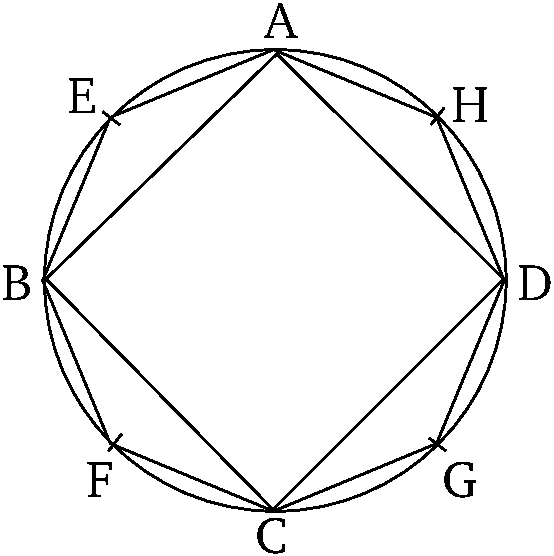
\includegraphics{Book12/fig10e.pdf}}

For if the cylinder is not three times the cone then the cylinder will be either more than three times, or less than three times, (the cone). Let it, first
of all, be  more than three times (the cone). And  let the square $ABCD$ be inscribed in circle $ABCD$ [Prop.~4.6].
So, square $ABCD$ is more than half of circle $ABCD$  [Prop.~12.2]. And let a prism
of equal height to the cylinder be set up on square $ABCD$. So, the prism set up is more than half of the
cylinder, inasmuch as  if we also circumscribe a square around circle $ABCD$ [Prop.~4.7] then the square inscribed in circle $ABCD$ is half of the circumscribed (square). And the  solids  set up on them are parallelepiped
prisms  of equal height.  And parallelepiped solids having the same height are to one
another as their bases [Prop.~11.32]. And, thus, the prism set up on square $ABCD$ is half
of the prism set up on the square circumscribed about circle $ABCD$. And the cylinder is less than the prism
set up on the square circumscribed about circle $ABCD$. Thus, the prism set up on square $ABCD$ of the
same height as the cylinder is more than half of the cylinder. Let the circumferences $AB$, $BC$, $CD$, and $DA$
be cut in half at points $E$, $F$, $G$, and $H$. And let $AE$, $EB$, $BF$, $FC$, $CG$, $GD$, $DH$,
and $HA$ be joined. And thus each of the triangles $AEB$, $BFC$, $CGD$, and $DHA$ is more than
half of the segment of circle $ABCD$ about it, as was shown previously [Prop.~12.2].
Let prisms of equal height to the cylinder be set up on each of the triangles $AEB$, $BFC$, $CGD$,
and $DHA$.  And each of the prisms set up is greater than the half part of the segment of the cylinder about it---inasmuch
as if we  draw (straight-lines) parallel to $AB$, $BC$, $CD$, and $DA$ through points $E$, $F$, $G$, and $H$
(respectively), and complete the parallelograms on $AB$, $BC$, $CD$, and $DA$, and set up parallelepiped solids
of equal height to the cylinder on them, then the prisms on triangles $AEB$, $BFC$, $CGD$, and $DHA$ are each half
of the set up (parallelepipeds). And the segments of the cylinder are less than the set up parallelepiped solids. 
Hence, the prisms on triangles $AEB$, $BFC$, $CGD$, and $DHA$ are also greater than half of the segments
of the cylinder about them. So (if) the remaining circumferences are cut in half, and straight-lines are joined,
and prisms of equal height to the cylinder are set up on each of the triangles, and this is done
continually,  then we will (eventually) leave some segments of the cylinder whose (sum) is less than the excess by which the
cylinder exceeds three times the cone [Prop.~10.1]. Let them be left, and let them be $AE$, $EB$, $BF$, $FC$, $CG$,
$GD$, $DH$, and $HA$. Thus, the remaining prism whose base (is) polygon $AEBFCGDH$, and height  the
same as the cylinder, is greater than three times the cone. But, the prism whose base is polygon $AEBFCGDH$,
and height the same as the cylinder,  is three times the pyramid whose base is polygon $AEBFCGDH$, and
apex the same as the cone [Prop.~12.7~corr.]. And thus the pyramid whose base [is] polygon 
$AEBFCGDH$, and apex the same as the cone, is greater than the cone having (as) base circle $ABCD$. But (it is)
also less. For it is encompassed by it. The very thing (is) impossible. Thus, the cylinder is not more than
three times the cone.

So, I say that neither (is) the cylinder less than three times the cone.

For, if possible, let the cylinder be less than three times the cone. Thus, inversely, the cone is greater than the third
part of the cylinder. So, let the square $ABCD$ be inscribed in circle $ABCD$  [Prop.~4.6]. Thus, square $ABCD$ is greater
than half of circle $ABCD$. 
And let a pyramid having the same apex as the cone be set up on square  $ABCD$. Thus, the pyramid set up
is greater than the half part of the cone, inasmuch as we showed previously that if we circumscribe a square
about the circle [Prop.~4.7] then the square $ABCD$ will be half of the square circumscribed about the circle [Prop.~12.2]. And if we set up   on the squares parallelepiped solids---which are also
called prisms---of the same height as the cone, then the (prism) set up on square $ABCD$ will be half of the (prism) set up on the square circumscribed
about the circle. For they are to one another as their bases [Prop.~11.32]. Hence, (the same) also (goes for) the thirds.  Thus, the pyramid whose base is square $ABCD$ is half of the pyramid set up on the square
circumscribed about the circle [Prop.~12.7~corr.]. And the pyramid set up on the square
circumscribed about the circle is greater than the cone. For it encompasses it. Thus, the pyramid whose
base is square $ABCD$, and apex the same as the cone, is greater than half of the cone. Let the circumferences $AB$,
$BC$, $CD$, and $DA$ be cut in half at points $E$, $F$, $G$, and $H$ (respectively).  And let $AE$, $EB$, $BF$,
$FC$, $CG$, $GD$, $DH$, and $HA$ be joined. And, thus, each of the triangles $AEB$, $BFC$,
$CGD$, and $DHA$ is greater than the half part of the segment of circle $ABCD$ about it [Prop.~12.2].
And let pyramids having the same apex as the cone be set up on each of the triangles $AEB$,
$BFC$, $CGD$, and $DHA$. And, thus, in the same way, each of the pyramids set up is more than the  half part of
the segment of the cone about it. So, (if) the remaining circumferences are cut in half, and straight-lines
are joined, and pyramids having the same apex as the cone are set up on each of the triangles, and this is
done continually, then we will (eventually) leave some segments of the cone 
whose (sum) is less than
the excess by which the cone exceeds the third part of the cylinder [Prop.~10.1]. 
Let them be left, and let them be the (segments) on $AE$, $EB$, $BF$, $FC$, $CG$, $GD$,
$DH$, and $HA$. Thus, the remaining pyramid whose base is polygon $AEBFCGDH$, and apex the
same as the cone, is greater than the third part of the cylinder. But, the pyramid whose base is
polygon $AEBFCGDH$, and apex the same as the cone, is the third part of the prism whose base
is polygon $AEBFCGDH$, and height the same as the cylinder [Prop.~12.7~corr.].
Thus, the prism whose base is polygon $AEBFCGDH$, and height the same as the cylinder, is greater than
the cylinder whose base is circle $ABCD$. But, (it is) also less. For it is encompassed by it. The very thing
is impossible. Thus, the cylinder is not less than three times the cone. And it was shown that neither (is it)
greater than three times (the cone). Thus, the cylinder (is) three times the cone. Hence, the cone is the
third part of the cylinder.

Thus, every cone is the third part of the cylinder which has the same base as it, and an equal height.
(Which is) the very thing it was required to show.}
\end{Parallel}

%%%%
%12.11
%%%%
\pdfbookmark[1]{Proposition 12.11}{pdf12.11}
\begin{Parallel}{}{}
\ParallelLText{
\begin{center}
{\large \ggn{11}.}
\end{center}\vspace*{-7pt}

\gr{Οἱ ὑπο τὸ α\kern -.7pt  ὐτὸ <ύψοξ >όντεξ κῶνοι καὶ κύλινδροι πρὸξ ἀλλήλουξ
εἰσὶν ὡξ αἱ βάσειξ.}

\gr{>'Εστωσαν ὑπὸ τὸ α\kern -.7pt  ὐτὸ <ύψοξ κῶνοι καὶ κύλινδροι, <ῶν
βάσειξ μὲν [εἰσιν] οἱ ΑΒΓΔ, ΕΖΗΘ κύκλοι, >άχονεξ δὲ οἱ ΚΛ, ΜΝ,
διάμετροι δὲ τῶν βάσεων αἱ ΑΓ, ΕΗ; λέγω, <ότι ἐστὶν ὡξ ὁ ΑΒΓΔ κύκλοξ πρὸξ τὸν ΕΖΗΘ κύκλον, ο<ύτωξ ὁ ΑΛ κῶνοξ πρὸξ
τὸν ΕΝ κῶνον.}

% Removed epsf size command
\centerline{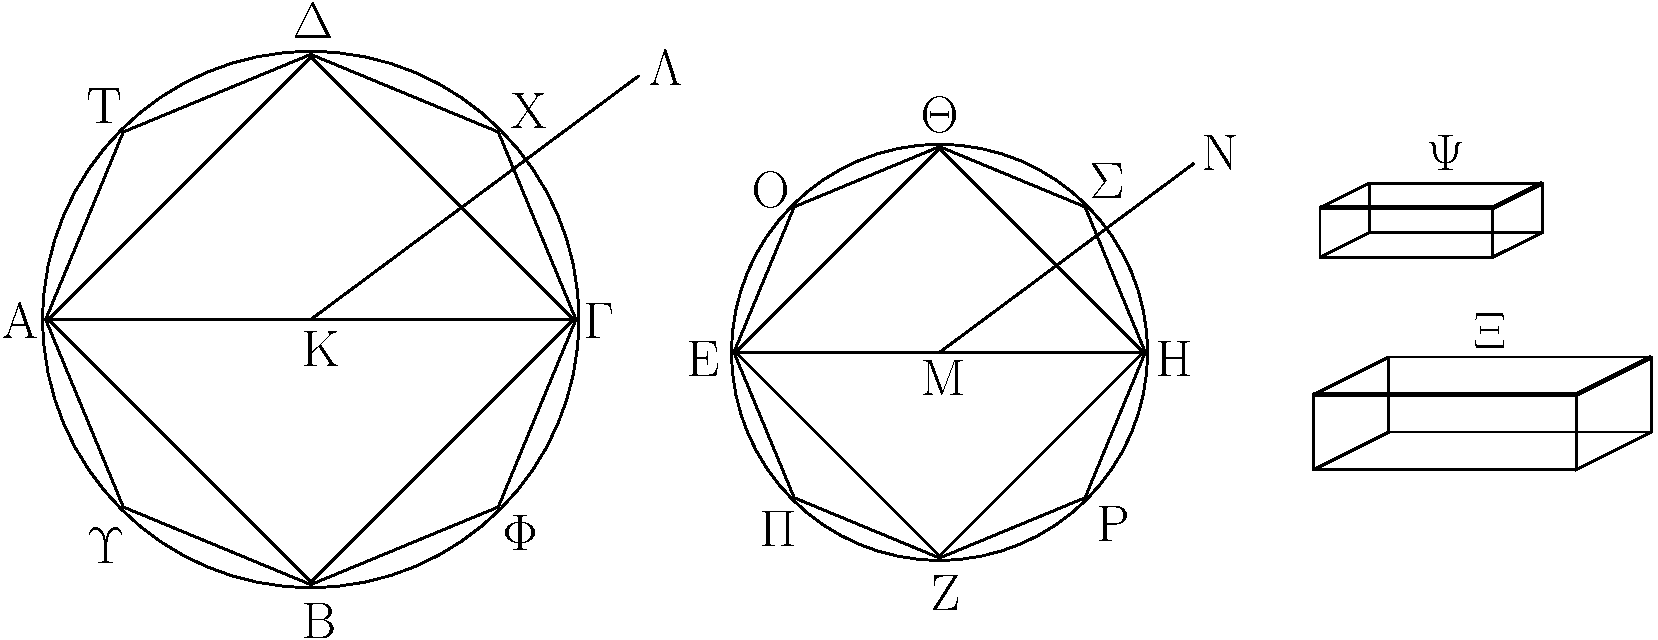
\includegraphics{Book12/fig11g.pdf}}

\gr{Εἰ γὰρ μ\kern -.7pt  ή, >έσται ὡξ ὁ ΑΒΓΔ κύκλοξ πρὸξ τὸν ΕΖΗΘ κύκλον,
ο<ύτωξ ὁ ΑΛ κῶνοξ >ήτοι πρὸξ >έλασσόν τι τοῦ ΕΝ κώνου
στερεὸν >ὴ πρὸξ μεῖζον. >έστω πρότερον πρὸξ >έλασσον
τὸ Χ, καὶ <ῶ| >έλασσόν ἐστι τὸ Χ στερεὸν τοῦ ΕΝ κώνου,
ἐκείνῳ >ίσον >έστω τὸ Ψ στερεόν; ὁ ΕΝ κῶνοξ >άρα >ίσοξ
ἐστὶ τοῖξ Χ, Ψ στερεοῖξ. ἐγγεγράφθω εἰξ τὸν ΕΖΗΘ κύκλον
τετράγωνον τὸ ΕΖΗΘ; τὸ >άρα τετράγωνον μεῖζόν ἐστιν >ὴ τὸ
<ήμισυ τοῦ κύκλου. ἀνεστάτω ἀπὸ τοῦ ΕΖΗΘ τετραγώνου
πυραμὶξ ἰσο"υψὴξ τῶ| κώνῳ; ἡ >άρα ἀνασταθεῖσα πυραμὶξ μείζων
ἐστὶν >ὴ τὸ <ήμισυ τοῦ κώνου, ἐπειδήπερ ἒαν περιγράψωμεν
περὶ τὸν κύκλον τετράγωνον, καὶ ἀπ> α\kern -.7pt  ὐτοῦ ἀναστήσωμεν
πυραμίδα ἰσο"υψῆ τῶ| κώνῳ, ἡ ἐγγραφεῖσα πυραμὶξ
<ήμισύ ἐστι τῆξ περιγραφείσηξ; πρὸξ ἀλλήλαξ γάρ εἰσιν ὡξ αἱ
βάσειξ; ἐλάττων δὲ ὁ κῶνοξ τῆξ περιγραφείσηξ πυραμίδοξ.
τετμ\kern -.5pt  ήσθωσαν αἱ ΕΖ, ΖΗ, ΗΘ, ΘΕ περιφέρειαι δίθα κατὰ τὰ Ο, Π, Ρ, Σ
σημεῖα, καὶ ἐπεζεύθθωσαν αἱ ΘΟ, ΟΕ, ΕΠ, ΠΖ, ΖΡ, ΡΗ, ΗΣ, ΣΘ.
<έκαστον >άρα τῶν ΘΟΕ, ΕΠΖ, ΖΡΗ, ΗΖΘ τριγώνων μεῖζόν
ἐστιν >ὴ τὸ <ήμισυ τοῦ καθ> ἑαυτὸ τμ\kern -.3pt  ήματοξ τοῦ κύκλου.
ἀνεστάτω ἐφ> ἑκάστου τῶν ΘΟΕ, ΕΠΖ, ΖΡΗ, ΗΣΘ
τριγώνων πυραμὶξ ἰσο"υψὴξ τῶ| κώνῳ; 
καὶ ἑκάστη >άρα τῶν ἀνασταθεισῶν πυραμίδων μείζων ἐστὶν >ὴ τὸ <ήμισυ τοῦ
καθ> ἑαυτὴν τμ\kern -.7pt  ήματοξ τοῦ κώνου. τέμνοντεξ δὴ τὰξ ὑπολειπομέναξ
περιφερείαξ δίθα καὶ ἐπιζευγνύντεξ εὐθείαξ καὶ ἀνιστάντεξ
ἐπὶ ἑκάστου τῶν τριγώνων πυραμίδαξ ἰσο"υψεῖξ τῶ| κώνῳ
καὶ ἀεὶ τοῦτο ποιοῦντεξ καταλείψομέν τινα ἀποτμ\kern -.7pt  ήματα τοῦ
κώνου, <ὰ >έσται ἐλάσσονα τοῦ Ψ στερεοῦ. 
λελείφθω, καὶ >έστω τὰ ἐπὶ τῶν ΘΟΕ, ΕΠΖ, ΖΡΗ, ΗΣΘ; 
λοιπὴ >άρα ἡ πυραμίξ, <ῆξ βάσιξ τὸ ΘΟΕΠΖΡΗΣ πολύγωνον, <ύψοξ δὲ τὸ α\kern -.7pt  ὐτὸ τῶ|
κώνῳ, μείζων ἐστὶ τοῦ Χ στερεοῦ.
 ἐγγεγράφθω καὶ εἰξ τὸν ΑΒΓΔ κύκλον τῶ| ΘΟΕΠΖΡΗΣ πολυγώνῳ <όμοιόν τε καὶ
ὁμοίωξ κείμενον πολύγωνον τὸ ΔΤΑΥΒΦΓΘ, καὶ ἀνεστάτω ἐπ>
α\kern -.7pt  ὐτοῦ πυραμὶξ ἰσο"υψὴξ τῶ| ΑΛ κώνῳ. 
ἐπεὶ ο>ῦν ἐστιν ὡξ τὸ ἀπὸ τῆξ ΑΓ πρὸξ τὸ ἀπὸ τῆξ ΕΗ, ο<ύτωξ τὸ
ΔΤΑΥΒΦΓΘ πολύγωνον πρὸξ τὸ ΘΟΕΠΖΡΗΣ
πολύγωνον, ὡξ δὲ τὸ ἀπὸ τῆξ ΑΓ πρὸξ τὸ ἀπὸ τῆξ ΕΗ, ο<ύτωξ
ὁ ΑΒΓΔ κύκλοξ πρὸξ τὸν ΕΖΗΘ κύκλον,
 καὶ ὡξ >άρα ὁ ΑΒΓΔ κύκλοξ πρὸξ τὸν ΕΖΗΘ κύκλον, ο<ύτωξ τὸ
 ΔΤΑΥΒΦΓΘ πολύγωνον πρὸξ τὸ ΘΟΕΠΖΡΗΣ πολύγωνον. 
 ὡξ δὲ ὁ ΑΒΓΔ κύκλοξ πρὸξ τὸν ΕΖΗΘ κύκλον, ο<ύτωξ ὁ ΑΛ
 κῶνοξ πρὸξ τὸ Χ στερεόν, 
 ὡξ δὲ τὸ ΔΤΑΥΒΦΓΘ πολύγωνον πρὸξ τὸ ΘΟΕΠΖΡΗΣ πολύγωνον, 
 ο<ύτωξ ἡ πυραμίξ, <ῆξ βάσιξ μὲν τὸ
 ΔΤΑΥΒΦΓΘ πολύγωνον, κορυφὴ δὲ τὸ Λ σημεῖον, πρὸξ τὴν πυραμίδα,
 <ῆξ βάσιξ μὲν τὸ
 ΘΟΕΠΖΡΗΣ πολύγωνον, κορυφὴ δὲ τὸ Ν σημεῖον. καὶ ὡξ >άρα ὁ
 ΑΛ κῶνοξ πρὸξ τὸ Χ 
 στερεόν,  ο<ύτωξ ἡ πυραμίξ, <ῆξ βάσιξ μὲν τὸ ΔΤΑΥΒΦΓΘ πολύγωνον,
κορυφὴ δὲ τὸ Λ σημεῖον, πρὸξ τὴν πυραμίδα, <ῆξ βάσιξ μὲν τὸ
ΘΟΕΠΖΡΗΣ πολύγωνον, κορυφὴ δὲ τὸ Ν σημεῖον; ἐναλλὰχ
>άρα ἐστὶν ὡξ ὁ ΑΛ κῶνοξ πρὸξ τὴν ἐν α\kern -.7pt  ὐτῶ|
πυραμίδα, ο<ύτωξ τὸ Χ στερεὸν πρὸξ τὴν ἐν τῶ| ΕΝ κώνῳ
πυραμίδα. μείζων δὲ ὁ ΑΛ κῶνοξ τῆξ ἐν α\kern -.7pt  ὐτῶ| πυραμίδοξ;
μεῖζον >άρα καὶ τὸ Χ στερεὸν τῆξ ἐν τῶ| ΕΝ κώνῳ πυραμίδοξ.
ἀλλὰ καὶ >έλασσον; <όπερ >άτοπον. οὐκ >άρα ἐστὶν ὡξ ὁ ΑΒΓΔ
κύκλοξ πρὸξ τὸν ΕΖΗΘ κύκλον, ο<ύτωξ ὁ ΑΛ κῶνοξ πρὸξ >έλασσόν τι
τοῦ ΕΝ κώνου στερεόν. ὁμοίωξ δὲ δείχομεν, <ότι οὐδέ
ἐστιν ὡξ ὁ ΕΖΗΘ κύκλοξ πρὸξ τὸν ΑΒΓΔ κύκλον, ο<ύτωξ
ὁ ΕΝ κῶνοξ πρὸξ >έλασσόν τι τοῦ ΑΛ κώνου στερεόν.}

\gr{Λέγω δή, <ότι οὐδέ ἐστιν ὡξ ὁ ΑΒΓΔ κύκλοξ πρὸξ τὸν
ΕΖΗΘ κύκλον, ο<ύτωξ ὁ ΑΛ κῶνοξ πρὸξ μεῖζόν τι τοῦ ΕΝ
κώνου στερεόν.}

\gr{Εἰ γὰρ δυνατόν, <έστω πρὸξ μεῖζον τὸ Χ; ἀνάπαλιν >άρα ἐστὶν ὡξ ὁ ΕΖΗΘ κύκλοξ πρὸξ τὸν ΑΒΓΔ κύκλον,  ο<ύτωξ τὸ Χ στερεὸν πρὸξ τὸν
ΑΛ κῶνον. ἀλλ> ὡξ τὸ Χ στερεὸν πρὸξ τὸν ΑΛ κῶνον, ο<ύτωξ ὁ ΕΝ
κῶνοξ πρὸξ >έλασσόν τι τοῦ ΑΛ κώνου στερεόν; καὶ ὡξ >άρα ὁ ΕΖΗΘ
κύκλοξ πρὸξ τὸν ΑΒΓΔ κύκλον, ο<ύτωξ ὁ ΕΝ κῶνοξ πρὸξ >έλασσόν τι τοῦ ΑΛ κώνου
στερεόν; <όπερ ἀδύνατον ἐδείθθη. οὐκ >άρα ἐστὶν ὡξ ὁ ΑΒΓΔ κύκλοξ πρὸξ τὸν ΕΖΗΘ κύκλον, ο<ύτωξ ὁ ΑΛ κῶνοξ πρὸξ μεῖζόν
τι τοῦ ΕΝ κώνου στερεόν. ἐδείθθη δέ, <ότι οὐδὲ πρὸξ >έλασσον;
>έστιν >άρα ὡξ ὁ ΑΒΓΔ κύκλοξ πρὸξ τὸν ΕΖΗΘ κύκλον, ο<ύτωξ
ὁ ΑΛ κῶνοξ πρὸξ τὸν ΕΝ κῶνον.}

\gr{Ἀλλ> ὡξ ὁ κῶνοξ πρὸξ τὸν κῶνον, ὁ κύλινδροξ πρὸξ τὸν
κύλινδρον; τριπλασίων γὰρ ἑκάτεροξ ἑκατέρου. καὶ ὡξ >άρα
ὁ ΑΒΓΔ κύκλοξ πρὸξ τὸν ΕΖΗΘ κύκλον, ο<ύτωξ οἱ ἐπ>
α\kern -.7pt  ὐτῶν ἰσο"υψεῖξ.}

\gr{Οἱ >άρα ὑπὸ τὸ α\kern -.7pt  ὐτὸ <ύψοξ >όντεξ κῶνοι καὶ κύλινδροι πρὸξ
ἀλλήλουξ εἰσὶν ὡξ αἱ βάσειξ; <όπερ >έδει δεῖχαι.}}

\ParallelRText{
\begin{center}
{\large Proposition 11}
\end{center}

Cones and cylinders having the same height are to one another as their bases.

Let there be cones and cylinders of the same height whose bases [are]  the circles $ABCD$ and $EFGH$,
axes $KL$ and $MN$, and diameters of the bases $AC$ and $EG$ (respectively). I say that as
circle $ABCD$ is to circle $EFGH$, so cone  $AL$ (is) to cone $EN$.

% Removed epsf size command
\centerline{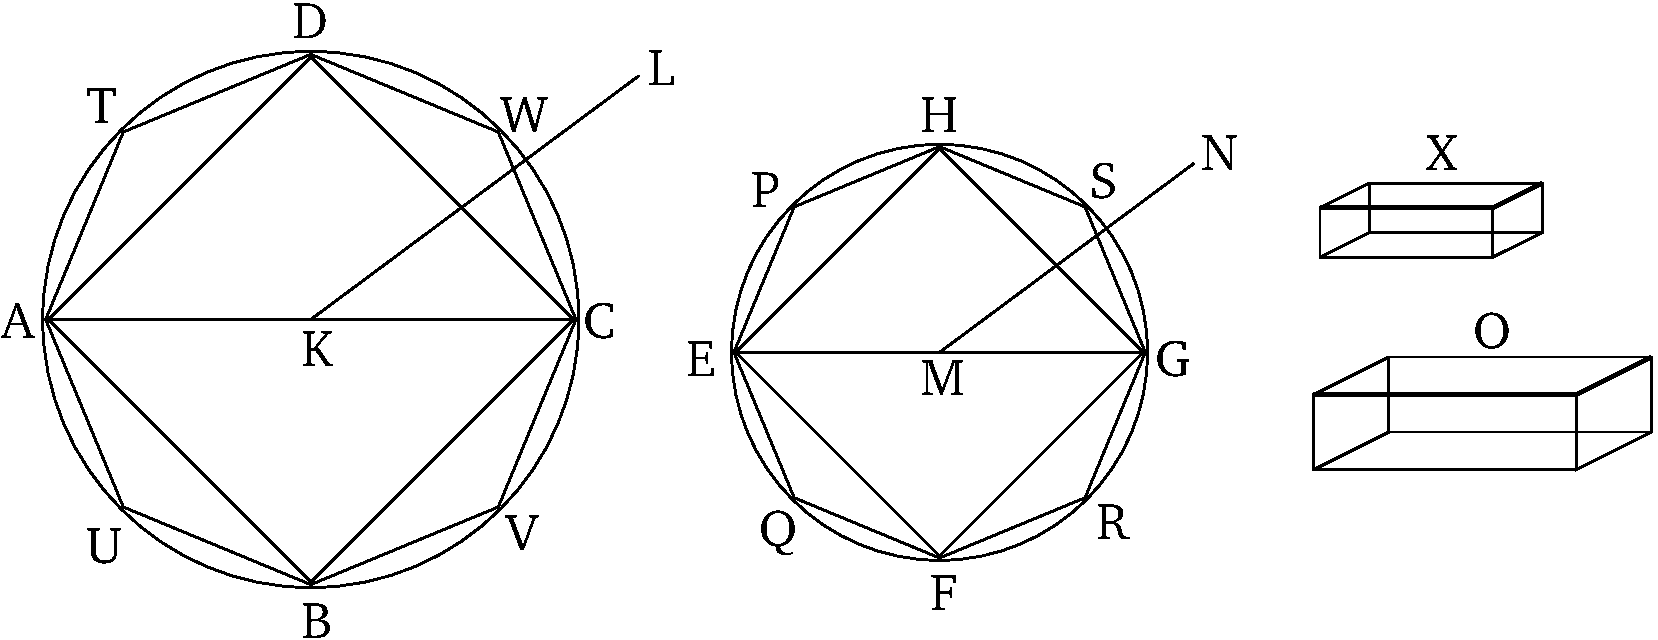
\includegraphics{Book12/fig11e.pdf}}

For if not, then as circle $ABCD$ (is) to circle $EFGH$, so cone $AL$ will be to some solid either less than, or
greater than, cone $EN$. Let it, first of all, be (in this ratio) to (some) lesser (solid), $O$. And let solid $X$ be equal to
that (magnitude) by which solid $O$ is less than cone $EN$. Thus, cone $EN$ is equal to (the sum of) solids
$O$ and $X$. Let the square $EFGH$ be inscribed in circle $EFGH$ [Prop.~4.6].
Thus, the square is greater than half of the circle [Prop.~12.2]. Let a pyramid
of the same height as the cone be set up on square $EFGH$. Thus, the pyramid set up is
greater than half of the cone, inasmuch as, if we circumscribe a square about the circle [Prop.~4.7], and set up  on it a pyramid of the same height as the cone, then the inscribed pyramid
is half of the circumscribed pyramid.  For they are to one another as their 
bases [Prop.~12.6]. And the cone (is) less than the circumscribed pyramid. 
Let the circumferences $EF$, $FG$, $GH$, and $HE$ be cut in half at points $P$, $Q$, $R$,
and $S$. And let $HP$, $PE$, $EQ$, $QF$, $FR$, $RG$, $GS$, and $SH$ be joined.
Thus, each of the triangles $HPE$, $EQF$, $FRG$, and $GSH$ is greater than half of the segment of
the circle about it [Prop.~12.2]. Let pyramids of the same height
as the cone be set up on each of the triangles $HPE$, $EQF$, $FRG$, and $GSH$.  And, thus, each of
the pyramids set up is greater than half of the segment of the cone about it [Prop.~12.10].
So, (if) the remaining circumferences are cut in half, and straight-lines are joined, and pyramids  of equal height to the cone are
set up on each of the triangles, and this is 
done continually, then we will (eventually) leave some segments of the cone (the sum of) which is less 
than solid $X$ [Prop.~10.1]. Let them be left, and let them be the
(segments) on $HPE$, $EQF$, $FRG$, and $GSH$. Thus, the remaining pyramid whose base is
polygon $HPEQFRGS$, and height the same as the cone, is greater than solid $O$ [Prop.~6.18]. 
And let the polygon $DTAUBVCW$, similar, and similarly laid out, to polygon $HPEQFRGS$, be
inscribed in circle $ABCD$. And on it let a pyramid of the same height as cone 
$AL$ be set up.
Therefore, since as the (square) on $AC$ is to the (square) on $EG$, so polygon $DTAUBVCW$ (is) to
polygon $HPEQFRGS$ [Prop.~12.1], and as the (square) on $AC$ (is) to the (square) on $EG$,
so circle $ABCD$ (is) to circle $EFGH$ [Prop.~12.2], thus as circle $ABCD$ (is) to
circle $EFGH$, so polygon $DTAUBVCW$ also (is) to polygon $HPEQFRGS$. And as circle $ABCD$ (is) to circle
$EFGH$, so cone $AL$ (is) to solid $O$. And as polygon $DTAUBVCW$ (is) to polygon $HPEQFRGS$, so the
pyramid whose base is polygon $DTAUBVCW$, and apex the point $L$, (is) to  the pyramid whose base is
polygon $HPEQFRGS$, and apex the point $N$ [Prop.~12.6]. And, thus, as cone $AL$ (is)
to solid $O$, so the pyramid whose base is $DTAUBVCW$, and apex the point $L$, (is) to  the pyramid whose base is
polygon $HPEQFRGS$, and apex the point $N$ [Prop.~5.11]. Thus, alternately, as cone $AL$ is to the pyramid within it, so solid $O$
(is) to the pyramid within cone $EN$ [Prop.~5.16]. But, cone $AL$ (is) greater than the
pyramid within it. Thus, solid $O$ (is) also greater than the pyramid within cone $EN$ [Prop.~5.14]. But,
(it is) also less. The very thing (is) absurd. Thus, circle $ABCD$ is not to circle $EFGH$, as cone $AL$
(is) to some solid less than cone $EN$. So, similarly, we can show that neither is circle $EFGH$
to circle $ABCD$, as cone $EN$ (is) to some solid less than cone $AL$.

So, I say that neither is circle $ABCD$ to circle $EFGH$, as cone $AL$ (is) to some solid greater than
cone $EN$.

For, if possible, let it be (in this ratio) to (some) greater (solid), $O$. Thus, inversely, as circle $EFGH$ is to circle
$ABCD$, so solid $O$ (is) to cone $AL$ [Prop.~5.7~corr.]. But, as solid $O$ (is) to cone $AL$, so cone $EN$ (is) to some
solid less than cone $AL$ [Prop.~12.2~lem.].  And, thus, as circle $EFGH$
(is)  to circle $ABCD$, so cone $EN$ (is) to some solid less than cone $AL$. The very thing was shown
(to be) impossible. Thus, circle $ABCD$ is not to circle $EFGH$, as cone $AL$ (is) to some solid greater than
cone $EN$. And, it was shown that neither (is it in this ratio) to (some) lesser (solid). Thus, as circle $ABCD$ is to circle
$EFGH$, so cone $AL$ (is) to cone $EN$.

But, as the cone (is) to the cone, (so) the cylinder (is) to the cylinder. For each (is) three times each [Prop.~12.10]. Thus, circle $ABCD$ (is) also to circle $EFGH$, as  (the ratio of the cylinders) on them (having) the
same height.

Thus, cones and cylinders having the same height are to one another as their bases. (Which is) the very thing
it was required to show.}
\end{Parallel}

%%%%
%12.12
%%%%
\pdfbookmark[1]{Proposition 12.12}{pdf12.12}
\begin{Parallel}{}{}
\ParallelLText{
\begin{center}
{\large \ggn{12}.}
\end{center}\vspace*{-7pt}

\gr{Οἱ <όμοιοι κῶνοι καὶ κύλινδροι πρὸξ ἀλλήλουξ ἐν τριπλασίονι λόγῳ
εἰσὶ τῶν ἐν ταῖξ βάσεσι διαμέτρων.}

\gr{>'Εστωσαν <όμοιοι κῶνοι καὶ κύλινδροι, <ῶν βάσειξ μὲν οἱ ΑΒΓΔ, ΕΖΗΘ
κύκλοι, διάμετροι δὲ τῶν βάσεων αἱ ΒΔ, ΖΘ, >άχονεξ δὲ τῶν κώνων καὶ
κυλίνδρων οἱ ΚΛ, ΜΝ; λέγω, <ότι ὁ κῶνοξ, ο<ῦ βάσιξ μέν [ἐστιν]
ὁ ΑΒΓΔ κύκλοξ, κορυφὴ δὲ τὸ Λ σημεῖον, πρὸξ τὸν κῶνον, ο<ῦ βάσιξ
μέν [ἐστιν] ὁ ΕΖΗΘ κύκλοξ, κορυφὴ δὲ τὸ Ν σημεῖον, τριπλασίονα
λόγον >έθει >ήπερ ἡ ΒΔ πρὸξ τὴν ΖΘ.}

% Removed epsf size command
\centerline{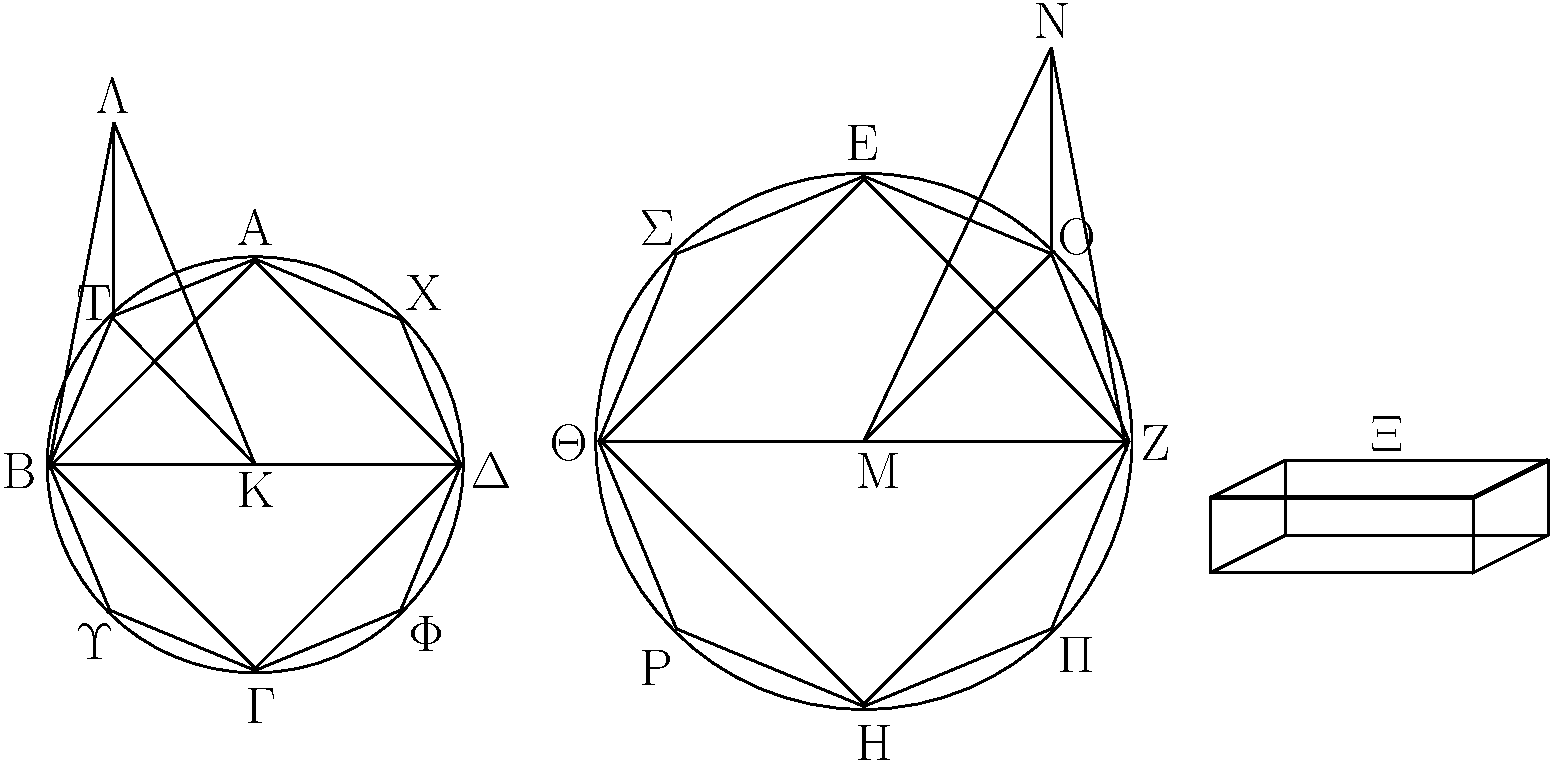
\includegraphics{Book12/fig12g.pdf}}

\gr{Εἰ γὰρ μ\kern -.7pt  ὴ >έθει ὁ ΑΒΓΔΛ κῶνοξ πρὸξ τὸν ΕΖΗΘΝ κῶνον πριπλασίονα
λόγον >ήπερ ἡ ΒΔ πρὸξ τὴν ΖΘ, <έχει ὁ ΑΒΓΔΛ κῶνοξ >ὴ πρὸξ >έλασσόν
τι τοῦ ΕΖΗΘΝ κώνου στερεὸν τριπλασίονα λόγον >ὴ πρὸξ μεῖζον. ἐθέτω
πρότερον πρὸξ >έλασσον τὸ Χ, καὶ ἐγγεγράφθω εἰξ τὸν ΕΖΗΘ κύκλον
τετράγωνον τὸ ΕΖΗΘ; τὸ >άρα ΕΖΗΘ τετράγωνον μεῖζόν ἐστιν >ὴ τὸ
<ήμισυ τοῦ ΕΖΗΘ κύκλου. καὶ ἀνεστάτω ἐπὶ τοῦ ΕΖΗΘ τετραγώνου
πυραμὶξ τὴν α\kern -.7pt  ὐτὴν κορυφὴν >έθουσα τῶ| κώνῳ; ἡ >άρα ἀνασταθεῖσα
πυραμὶξ μείζων ἐστὶν >ὴ τὸ <ήμισυ μέροξ τοῦ κώνου. τετμ\kern -.5pt  ήσθωσαν
δὴ αἱ ΕΖ, ΖΗ, ΗΘ, ΘΕ περιφέρειαι δίθα κατὰ τὰ Ο, Π, Ρ, Σ σημεῖα,
καὶ ἐπεζεύθθωσαν αἱ ΕΟ, ΟΖ, ΖΠ, ΠΗ, ΗΡ, ΡΘ, ΘΣ, ΣΕ. καὶ <έκαστον >άρα
τῶν ΕΟΖ, ΖΠΗ, ΗΡΘ, ΘΣΕ τριγώνων μεῖζόν ἐστιν >ὴ τὸ <ήμισυ
μέροξ τοῦ καθ> ἑαυτὸ τμ\kern -.3pt  ήματοξ τοῦ ΕΖΗΘ κύκλου. καὶ ἀνεστάτω
ἐφ> ἑκάστου τῶν ΕΟΖ, ΖΠΗ, ΗΡΘ, ΘΣΕ τριγώνων
πυραμὶξ τὴν α\kern -.7pt  ὐτὴν κορυφὴν >έθουσα τῶ| κώνῳ; καὶ ἑκάστη >άρα τῶν
ἀνασταθεισῶν πυραμίδων μείζων ἐστὶν >ὴ τὸ <ήμισυ μέροξ τοῦ καθ> ἑαυτὴν
τμ\kern -.7pt  ήματοξ τοῦ κώνου.
 τέμνοντεξ δὴ τὰξ ὑπολειπομέναξ περιφερείαξ
δίθα καὶ ἐπιζευγνύντεξ εὐθείαξ καὶ ἀνιστάντεξ ἐφ> ἑκάστου
τῶν τριγώνων πυραμίδαξ τὴν α\kern -.7pt  ὐτὴν κορυφὴν ἐθούσαξ τῶ| κώνῳ καὶ
τοῦτο ἀεὶ ποιοῦντεξ καταλείψομέν τινα ἀποτμ\kern -.7pt  ήματα τοῦ κώνου, <ὰ >έσται
ἐλάσσονα τῆξ ὑπεροθῆξ, <ῆ| ὑπερέθει ὁ ΕΖΗΘΝ κῶνοξ τοῦ Χ στερεοῦ.
λελείφθω, καὶ >έστω τὰ ἐπὶ τῶν ΕΟ, ΟΖ, ΖΠ, ΠΗ, ΗΡ, ΡΘ, ΘΣ, ΣΕ;
λοιπὴ >άρα ἡ πυραμίξ, <ῆξ βάσιξ μέν ἐστι τὸ ΕΟΖΠΗΡΘΣ πολύγωνον,
κορυφὴ δὲ τὸ Ν σημεῖον, μείζων ἐστὶ τοῦ Χ στερεοῦ. ἐγγεγράφθω
καὶ εἰξ τὸν ΑΒΓΔ κύκλον τῶ| ΕΟΖΠΗΡΘΣ πολυγώνῳ <όμοιόν τε καὶ
ὁμοίωξ κείμενον πολύγωνον τὸ ΑΤΒΥΓΦΔΘ, καὶ ἀνεστάτω ἐπὶ
τοῦ ΑΤΒΥΓΦΔΘ πολυγώνου πυραμὶξ τὴν α\kern -.7pt  ὐτὴν κορυφὴν >έθουσα
τῶ| κώνῳ, καὶ τῶν μὲν περιεθόντων τὴν πυραμίδα, <ῆξ βάσιξ
μέν ἐστι τὸ ΑΤΒΥΓΦΔΘ πολύγωνον, κορυφὴ δὲ τὸ Λ σημεῖον,
<ὲν τρίγωνον >έστω τὸ ΛΒΤ, τῶν δὲ περειθόντων τὴν πυραμίδα,
<ῆξ βάσιξ μέν ἐστι τὸ ΕΟΖΠΗΡΘΣ πολύγωνον, κορυφὴ δὲ τὸ
Ν σημεῖον, <ὲν τρίγωνον >έστω τὸ ΝΖΟ, καὶ ἐπεζεύθθωσαν
αἱ ΚΤ, ΜΟ. καὶ ἐπεὶ <όμοιόξ ἐστιν ὁ ΑΒΓΔΛ κῶνοξ τῶ|
ΕΖΗΘΝ κώνῳ,  >έστιν >άρα ὡξ ἡ ΒΔ πρὸξ τὴν ΖΘ, ο<ύτωξ
ὁ ΚΛ >άχων πρὸξ τὸν ΜΝ >άχονα. ὡξ δὲ ἡ ΒΔ πρὸξ τὴν ΖΘ,
ο<ύτωξ ἡ ΒΚ πρὸξ τὴν ΖΜ; καὶ ὡξ >άρα ἡ ΒΚ πρὸξ τὴν ΖΜ, 
ο<ύτωξ ἡ ΚΛ πρὸξ τὴν ΜΝ. καὶ ἐναλλὰχ ὡξ ἡ ΒΚ πρὸξ τὴν
ΚΛ, ο<ύτωξ ἡ ΖΜ πρὸξ τὴν ΜΝ. καὶ περὶ >ίσαξ γωνίαξ τὰξ
ὑπὸ ΒΚΛ, ΖΜΝ αἱ πλευραὶ ἀνάλογόν εἰσιν; <όμοιον
>άρα ἐστὶ τὸ ΒΚΛ τρίγωνον τῶ| ΖΜΝ τριγώνῳ. 
πάλιν, ἐπεί ἐστιν ὡξ ἡ ΒΚ
πρὸξ τὴν ΚΤ, ο<ύτωξ ἡ ΖΜ πρὸξ τὴν ΜΟ, καὶ περὶ >ίσαξ γωνίαξ τὰξ ὑπὸ
ΒΚΤ, ΖΜΟ, ἐπειδήπερ, <ὸ μέροξ ἐστὶν ἡ ὑπὸ ΒΚΤ γωνία τῶν πρὸξ
τῶ| Κ κέντρῳ τεσσάρων ὀρθῶν, τὸ α\kern -.7pt  ὐτὸ μέροξ ἐστὶ καὶ ἡ ὑπὸ ΖΜΟ
γωνία τῶν πρὸξ τῶ| Μ κέντρῳ τεσσάρων ὀρθῶν; ἐπεὶ ο~ὐν περὶ
>ίσαξ γωνίαξ αἱ πλευραὶ ἀνάλογόν εἰσιν, <όμοιον >άρα ἐστι τὸ  ΒΚΤ τρίγωνον
τῶ| ΖΜΟ τριγώνῳ. πάλιν, ἐπεὶ ἐδείθθη ὡξ ἡ ΒΚ πρὸξ τὴν ΚΛ,
ο<ύτωξ ἡ ΖΜ πρὸξ τὴν ΜΝ, >ίση δὲ ἡ μὲν ΒΚ τῆ| ΚΤ, ἡ δὲ ΖΜ τῆ|
ΟΜ, >έστιν >άρα ὡξ ἡ ΤΚ πρὸξ τὴν ΚΛ, ο<ύτωξ ἡ ΟΜ πρὸξ τὴν ΜΝ. καὶ
περὶ >ίσαξ γωνίαξ τὰξ ὑπὸ ΤΚΛ, ΟΜΝ; ὀρθαὶ γάρ; αἱ πλευραὶ ἀνάλογόν
εἰσιν; <όμοιον >άρα ἐστὶ τὸ ΛΚΤ τρίγωνον τῶ| ΝΜΟ τριγώνῳ. καὶ
ἐπεὶ διὰ τὴν ὁμοιότητα τῶν ΛΚΒ, ΝΜΖ τριγώνων ἐστὶν ὡξ ἡ ΛΒ
πρὸξ τὴν ΒΚ, ο<ύτωξ ἡ ΝΖ πρὸξ τὴν ΖΜ, διὰ δὲ τὴν ὁμοιότητα τῶν 
ΒΚΤ,
ΖΜΟ τριγώνων ἐστὶν ὡξ ἡ ΚΒ πρὸξ τὴν ΒΤ, ο<ύτωξ ἡ ΜΖ πρὸξ τὴν ΖΟ,
δι> >ίσου >άρα ὡξ ἡ ΛΒ πρὸξ τὴν ΒΤ, ο<ύτωξ ἡ ΝΖ πρὸξ τὴν ΖΟ. πάλιν,
ἐπεὶ διὰ τὴν ομοιότητα τῶν ΛΤΚ, ΝΟΜ τριγώνων ἐστὶν ὡξ ἡ ΛΤ πρὸξ
τὴν ΤΚ, ο<ύτωξ ἡ ΝΟ πρὸξ τὴν ΟΜ, διὰ δὲ τὴν ὁμοιότητα τῶν ΤΚΒ, ΟΜΖ
τριγώνων ἐστὶν ὡξ ἡ ΚΤ πρὸξ τὴν ΤΒ, ο<ύτωξ ἡ ΜΟ πρὸξ τὴν ΟΖ, δι>
>ίσου >άρα ὡξ ἡ ΛΤ πρὸξ τὴν ΤΒ, ο<ύτωξ ἡ ΝΟ πρὸξ τὴν ΟΖ. ἐδείθθη
δὲ καὶ ὡξ ἡ ΤΒ πρὸξ τὴν ΒΛ, ο<ύτωξ ἡ ΟΖ πρὸξ τὴν ΖΝ. δι> >ίσου
>άρα ὡξ ἡ ΤΛ πρὸξ τὴν ΛΒ, ο<ύτωξ ἡ ΟΝ πρὸξ τὴν ΝΖ. τῶν ΛΤΒ, ΝΟΖ
>άρα τριγώνων ἀνάλογόν εἰσιν αἱ πλευραί; ἰσογώνια >άρα ἐστὶ τὰ ΛΤΒ, ΝΟΖ
τρίγωνα; <ώστε καὶ <όμοια. καὶ πυραμὶξ >άρα, <ῆξ βάσιξ μὲν τὸ ΒΚΤ τρίγωνον,
κορυφὴ δὲ τὸ Λ σημεῖον, ὁμοία ἐστὶ πυραμίδι, <ῆξ βάσιξ μὲν τὸ ΖΜΟ
τρίγωνον, κορυφὴ δὲ τὸ Ν σημεῖον; ὑπὸ γὰρ <όμοίων ἐπιπέδων περιέθονται
>ίσων τὸ πλῆθοξ. αἱ δὲ <όμοιαι πυραμίδεξ καὶ τριγώνουξ >έθουσαι βάσειξ
ἐν τριπλασίονι λόγῳ εἰσὶ τῶν ὁμολόγων πλευρῶν. ἡ >άρα ΒΚΤΛ πυραμὶξ
πρὸξ τὴν ΖΜΟΝ πυραμίδα τριπλασίονα λόγον >έθει >ήπερ ἡ ΒΚ πρὸξ 
τὴν ΖΜ.
ὁμοίωξ δὴ ἐπιζευγνύντεξ ἀπὸ τῶν Α, Θ, Δ, Φ, Γ, Υ ἐπὶ τὸ Κ εὐθείαξ
καὶ ἀπὸ  τῶν Ε, Σ, Θ, Ρ, Η, Π ἐπὶ τὸ Μ καὶ ἀνιστάντεξ ἐφ> ἑκάστου
τῶν τριγώνων πυραμίδαξ τὴν α\kern -.7pt  ὐτὴν κορυφὴν ἐθούσαξ τοῖξ κώνοιξ
δείχομεν, <ότι καὶ ἑκάστη τῶν ὁμοταγῶν πυραμίδων πρὸξ ἑκάστην ὁμοταγῆ
πυραμίδα τριπλασίονα λόγον <έχει >ήπερ ἡ ΒΚ ὁμόλογοξ πλευρὰ πρὸξ τὴν ΖΜ
ὁμόλογον πλευράν, τουτέστιν >ήπερ ἡ ΒΔ πρὸξ τὴν ΖΘ. καὶ ὡξ <ὲν τῶν
ἡγουμένων πρὸξ <ὲν τῶν ἑπομένων, ο<ύτωξ <άπαντα τὰ ἡγούμενα
πρὸξ <άπαντα τὰ ἑπόμενα; >έστιν >άρα καὶ ὡξ ἡ ΒΚΤΛ πυραμὶξ πρὸξ
τὴν ΖΜΟΝ πυραμίδα, ο<ύτωξ ἡ <όλη πυραμίξ, <ῆξ βάσιξ τὸ ΑΤΒΥΓΦΔΘ πολύγωνον,
κορυφὴ δὲ τὸ Λ σημεῖον, πρὸξ τὴν <όλην πυραμίδα, <ῆξ βάσιξ μὲν τὸ ΕΟΖΠΗΡΘΣ πολύγωνον,
κορυφὴ δὲ τὸ Ν σημεῖον; <ώστε καὶ πυραμίξ, <ῆξ βάσιξ μὲν τὸ ΑΤΒΥΓΦΔΘ, κορυφὴ
δὲ τὸ Λ, πρὸξ τὴν πυραμίδα, <ῆξ βάσιξ [μὲν] τὸ ΕΟΖΠΗΡΘΣ πολύγωνον, κορυφὴ
δὲ τὸ Ν σημεῖον, τριπλασίονα λόγον >έθει >ήπερ ἡ ΒΔ πρὸξ τὴν ΖΘ. ὑπόκειται δὲ καὶ
ὁ κῶνοξ, ο<ῦ βάσιξ [μὲν]
ὁ ΑΒΓΔ κύκλοξ, κορυφὴ δὲ τὸ Λ σημεῖον, πρὸξ τὸ Χ στερεὸν τριπλασίονα λόγον >έθων
>ήπερ ἡ ΒΔ πρὸξ τὴν ΖΘ;  >έστιν >άρα ὡξ ὁ κῶνοξ, ο<ῦ βάσιξ μέν ἐστιν ὁ ΑΒΓΔ κύκλοξ,
κορυφὴ δὲ τὸ Λ, πρὸξ τὸ Χ στερεόν, ο<ύτωξ ἡ πυραμίξ, <ῆξ βάσιξ μὲν τὸ ΑΤΒΥΓΦΔΘ [πολύγωνον],
κορυφὴ δὲ τὸ Λ, πρὸξ τὴν πυραμίδα, <ῆξ βάσιξ μέν ἐστι τὸ ΕΟΖΠΗΡΘΣ πολύγωνον, κορυφὴ
δὲ τὸ Ν; ἐναλλὰχ >άρα, ὡξ ὁ κῶνοξ, ο<ῦ βάσιξ μὲν ὁ ΑΒΓΔ κύκλοξ, κορυφὴ δὲ
τὸ Λ, πρὸξ τὴν ἐν α\kern -.7pt  ὐτῶ| πυραμίδα, <ῆξ βάσιξ μὲν τὸ ΑΤΒΥΓΦΔΘ πολύγωνον, κορυφὴ
δὲ τὸ Λ, ο<ύτωξ τὸ Χ [στερεὸν] πρὸξ τὴν πυραμίδα, <ῆξ βάσιξ μέν ἐστι τὸ ΕΟΖΠΗΡΘΣ
πολύγωνον, κορυφὴ δὲ τὸ Ν. μείζων δὲ ὁ εἰρημένοξ κῶνοξ τῆξ ἐν α\kern -.7pt  ὐτῶ|
πυραμίδοξ; ἐμπεριέθει γὰρ α\kern -.7pt  ὐτὴν. μεῖζον >άρα καὶ τὸ Χ στερεὸν τῆξ πυραμίδοξ, <ῆξ βάσιξ
μέν ἐστι τὸ ΕΟΖΠΗΡΘΣ πολύγωνον, κορυφὴ δὲ τὸ Ν. ἀλλὰ καὶ >έλαττον; <όπερ ἐστὶν ἀδύνατον.
οὐκ >άρα ὁ κῶνοξ, ο<ῦ βάσιξ ὁ ΑΒΓΔ κύκλοξ, κορυφὴ δὲ τὸ Λ [σημεῖον], πρὸξ >έλαττόν
τι τοῦ κώνου στερεόν, ο<ῦ βάσιξ μὲν ὁ ΕΖΗΘ κύκλοξ, κορυφὴ δὲ τὸ Ν σημεῖον, τριπλασίονα
λόγον >έθει >ήπερ ἡ ΒΔ πρὸξ τὴν ΖΘ. ὁμοίωξ δὴ δείχομεν, <ότι οὐδὲ ὁ ΕΖΗΘΝ κῶνοξ
πρὸξ >έλαττόν τι τοῦ ΑΒΓΔΛ κώνου στερεὸν τριπλασίονα λόγον >έθει >ήπερ ἡ ΖΘ πρὸξ τὴν ΒΔ.}

\gr{Λέγω δή, <ότι οὐδὲ ὁ ΑΒΓΔΛ κῶνοξ πρὸξ μεῖζόν τι τοῦ ΕΖΗΘΝ κώνου στερεὸν τριπλασίονα
λόγον >έθει >ήπερ ἡ ΒΔ πρὸξ τὴν ΖΘ.}

\gr{Εἰ γὰρ δυνατόν, ἐθέτω πρὸξ μεῖζον τὸ Χ. ἀνάπαλιν >άρα τὸ Χ στερεὸν πρὸξ τὸν ΑΒΓΔΛ
κῶνον τριπλασίονα λόγον >έθει >ήπερ ἡ ΖΘ πρὸξ τὴν ΒΔ. ὡξ δὲ τὸ Χ στερεὸν πρὸξ τὸν ΑΒΓΔΛ
κῶνον, ο<ύτωξ ὁ ΕΖΗΘΝ κῶνοξ πρὸξ >έλαττόν τι τοῦ ΑΒΓΔΛ κώνου στερεόν. καὶ ὁ ΕΖΗΘΝ
>άρα κῶνοξ πρὸξ >έλαττόν τι τοῦ ΑΒΓΔΛ κώνου στερεὸν τριπλασίονα λόγον >έθει >ήπερ ἡ
ΖΘ πρὸξ τὴν ΒΔ; <όπερ ἀδύνατον ἐδείθθη. οὐκ >άρα ὁ ΑΒΓΔΛ κῶνοξ πρὸξ μεῖζόν τι
τοῦ ΕΖΗΘΝ κώνου στερεὸν τριπλασίονα λόγον >έθει >ήπερ ἡ ΒΔ πρὸξ τὴν ΖΘ. ἐδείθθη
δέ, <ότι οὐδὲ πρὸξ >έλαττον. ὁ ΑΒΓΔΛ >άρα κῶνοξ πρὸξ τὸν ΕΖΗΘΝ κῶνον τριπλασίονα
λόγον >έθει >ήπερ ἡ ΒΔ πρὸξ τὴν ΖΘ.}

\gr{Ὡξ δὲ ὁ κῶνοξ πρὸξ τὸν κῶνον, ὁ κύλινδροξ πρὸξ τὸν κύλινδρον; τριπλάσιοξ γὰρ ὁ κύλινδροξ
τοῦ κώνου ὁ ἐπὶ  τῆξ α\kern -.7pt  ὐτῆξ βάσεωξ τῶ| κώνῳ καὶ ἰσο"υψὴξ α\kern -.7pt  ὐτῶ|. καὶ ὁ κύλινδροξ >άρα πρὸξ τὸν
κύλινδρον τριπλασίονα λόγον >έθει >ήπερ ἡ ΒΔ πρὸξ τὴν ΖΘ.}

\gr{Οἱ >άρα <όμοιοι κῶνοι καὶ κύλινδροι πρὸξ ἀλλήλουξ ἐν τριπλασίονι λόγῳ εἰσὶ τῶν ἐν ταῖξ
βάσεσι διαμέτρων; <όπερ >έδει δεῖχαι.}}

\ParallelRText{
\begin{center}
{\large Proposition 12}
\end{center}

Similar cones and cylinders are to one another in the cubed ratio of
the diameters of their bases.

Let there be similar cones and cylinders of which the bases (are) the circles $ABCD$ and $EFGH$, the diameters of the bases (are) $BD$ and $FH$,
and the axes of the cones and cylinders (are)  $KL$ and $MN$ (respectively). I say that the cone whose base [is] circle $ABCD$, and apex the
point $L$,  has to the cone whose base [is] circle $EFGH$, and apex the point $N$,  the cubed ratio  that $BD$ (has) to $FH$.

% Removed epsf size command
\centerline{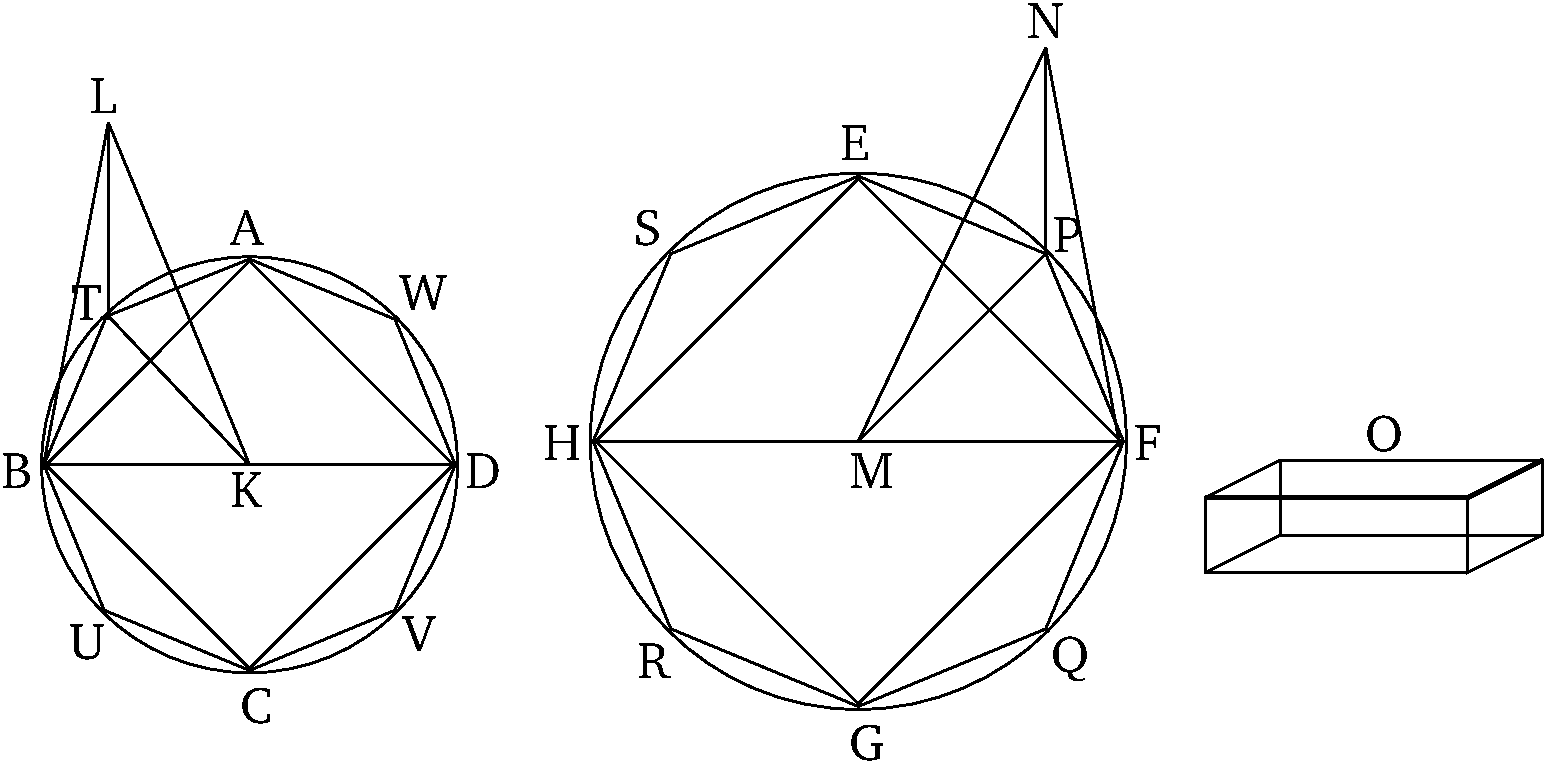
\includegraphics{Book12/fig12e.pdf}}

For if cone $ABCDL$ does not have to cone $EFGHN$ the cubed ratio that $BD$ (has) to $FH$ then cone $ABCDL$ will  have the
cubed ratio to some solid either less than, or greater than, cone $EFGHN$. Let it, first of all, have (such a  ratio) to
(some) lesser (solid), $O$. And let the square $EFGH$ be inscribed in circle $EFGH$ [Prop.~4.6]. 
Thus, square $EFGH$ is greater than half of circle $EFGH$ [Prop.~12.2]. And let a pyramid having the
same apex as the cone be set up on square $EFGH$. Thus, the pyramid set up is greater than the half part of the cone [Prop.~12.10]. So, let the circumferences $EF$, $FG$, $GH$, and $HE$ be cut in half at points $P$, $Q$, $R$, and $S$ (respectively). 
And let $EP$, $PF$, $FQ$, $QG$, $GR$, $RH$, $HS$, and $SE$ be
joined. And, thus, each of the triangles $EPF$, $FQG$, $GRH$, and $HSE$
is greater than the half part of the segment of circle $EFGH$ about it  [Prop.~12.2]. And let a pyramid having the same apex as
the cone be set up on each of the triangles $EPF$, $FQG$, $GRH$, and $HSE$. And thus each of the pyramids set up is greater than
the half part of the segment of the cone about it [Prop.~12.10]. So, (if) the the remaining circumferences are cut in half, and 
straight-lines are joined, and pyramids having the same apex as the cone are set up on each of 
the triangles, and this is done continually, then we will (eventually) leave some segments of the 
cone whose (sum) is less than the excess by which cone $EFGHN$ exceeds solid $O$ [Prop.~10.1].
Let them be left, and let them be the (segments) on $EP$, $PF$, $FQ$, $QG$, $GR$, $RH$, $HS$, and $SE$. Thus, the remaining
pyramid whose base is polygon $EPFQGRHS$, and apex the point $N$, is greater than solid $O$.  And let the polygon
$ATBUCVDW$, similar, and similarly laid out, to polygon $EPFQGRHS$, be inscribed in circle $ABCD$ [Prop.~6.18].
And let a pyramid having the same apex as the cone be set up on polygon $ATBUCVDW$. And let $LBT$ be one
of the triangles containing the pyramid whose base is polygon $ATBUCVDW$, and apex the point $L$. And let
$NFP$ be one of the triangles containing the pyramid whose base is triangle $EPFQGRHS$, and apex the point
$N$. And let $KT$ and $MP$ be joined. And since cone $ABCDL$ is similar to cone $EFGHN$, thus as
$BD$ is to $FH$, so axis $KL$ (is) to axis $MN$ [Def.~11.24].  And as $BD$ (is) to
$FH$, so $BK$ (is) to $FM$. And, thus, as $BK$ (is) to $FM$, so $KL$ (is) to $MN$. And, alternately, as $BK$ (is)
to $KL$, so $FM$ (is) to $MN$ [Prop.~5.16]. And the sides around the equal angles $BKL$ and
$FMN$ are proportional. Thus, triangle $BKL$ is similar to triangle $FMN$
[Prop.~6.6]. Again, since as $BK$ (is) to $KT$, so
$FM$ (is) to $MP$, and (they are) about the equal angles $BKT$ and $FMP$, inasmuch as whatever part angle $BKT$
is of the four right-angles at the center $K$, angle $FMP$ is also the same part of the four right-angles at the  center $M$. 
Therefore, since the sides about equal angles are proportional,  triangle $BKT$ is thus similar to traingle $FMP$ [Prop.~6.6].
Again, since it was shown that as $BK$ (is) to $KL$, so $FM$ (is) to $MN$, and $BK$ (is) equal to $KT$, and
$FM$ to $PM$, thus as $TK$ (is) to $KL$, so $PM$ (is) to $MN$. And the sides about the equal angles
$TKL$ and $PMN$---for (they are both) right-angles---are proportional.  Thus, triangle $LKT$ (is) similar to
triangle $NMP$ [Prop.~6.6]. And since, on account of the similarity of triangles $LKB$ and
$NMF$, as $LB$ (is) to $BK$, so $NF$ (is) to $FM$, and, on account of the  similarity of triangles $BKT$ and
$FMP$, as $KB$ (is) to $BT$, so $MF$ (is) to $FP$ [Def.~6.1], thus, via equality, as $LB$ (is)
to $BT$, so $NF$ (is) to $FP$ [Prop.~5.22]. Again, since, on account of the similarity of
triangles $LTK$ and $NPM$, as $LT$ (is) to $TK$, so $NP$ (is) to $PM$, and, on account of the similarity of
triangles $TKB$ and $PMF$, as $KT$ (is) to $TB$, so $MP$ (is) to $PF$, thus, via equality,  as $LT$ (is) to $TB$, so
$NP$ (is) to $PF$ [Prop.~5.22]. And it was shown that as $TB$ (is) to $BL$, so $PF$ (is) to $FN$.
 Thus, via equality, as $TL$ (is) to $LB$, so $PN$ (is) to $NF$ [Prop.~5.22]. Thus, the sides of triangles
 $LTB$ and $NPF$ are proportional. Thus, triangles $LTB$ and $NPF$ are equiangular [Prop.~6.5]. 
 And, hence, (they are) similar [Def.~6.1]. And, thus, the pyramid whose base is triangle $BKT$, and
 apex the point $L$, is similar to the pyramid whose base is triangle $FMP$, and apex the point $N$. For they are contained
 by equal numbers of similar planes [Def.~11.9]. And similar pyramids which also have triangular
 bases are in the cubed ratio of corresponding sides [Prop.~12.8]. Thus, pyramid
 $BKTL$ has to pyramid $FMPN$ the cubed ratio that $BK$ (has) to $FM$. So, similarly, joining
 straight-lines from (points) $A$, $W$, $D$, $V$, $C$, and $U$ to (center) $K$, and from (points) $E$, $S$, $H$, $R$,
 $G$,  and $Q$ to (center) $M$, and setting up pyramids having the same apexes as the cones on each of the triangles (so formed), we can also show
 that each of the pyramids (on base $ABCD$ taken) in order will have to each of the pyramids (on base $EFGH$ taken) in order the cubed ratio that the corresponding side
 $BK$ (has) to the corresponding side $FM$---that is to say, that $BD$ (has) to $FH$. And (for two sets of proportional magnitudes) as one of the leading
 (magnitudes is) to one of the following, so (the sum of) all of the leading 
 (magnitudes is) to (the sum of) all of the
 following (magnitudes) [Prop.~5.12]. And, thus, as pyramid $BKTL$ (is) to pyramid $FMPN$,
 so the whole pyramid whose base is polygon $ATBUCVDW$, and apex the point $L$, (is) to the whole pyramid
 whose base is polygon $EPFQGRHS$, and apex the point $N$. And, hence, the pyramid whose base is polygon $ATBUCVDW$, and apex the point $L$, has to the pyramid
 whose base is polygon $EPFQGRHS$, and apex the point $N$, the cubed ratio that $BD$ (has) to $FH$. And it was also assumed that the cone whose base is circle $ABCD$, and apex the point $L$, has to solid $O$ the cubed ratio that $BD$ (has)
 to $FH$. Thus, as the cone whose base is circle $ABCD$, and apex the point $L$, is to solid $O$, so the pyramid
 whose base (is) [polygon] $ATBUCVDW$, and apex the point $L$, (is) to the pyramid whose base is polygon $EPFQGRHS$, and apex the point $N$. Thus, alternately, as the cone whose base (is) circle $ABCD$, and apex the point $L$, (is)
 to the pyramid within it whose base (is) the polygon $ATBUCVDW$, and apex the point $L$, so the [solid] $O$ (is)
 to the pyramid whose base is polygon  $EPFQGRHS$, and apex the point $N$ [Prop.~5.16]. And the aforementioned cone (is)
 greater than the pyramid within it. For it encompasses it. Thus, solid $O$ (is) also greater than the pyramid whose base is polygon  $EPFQGRHS$, and apex the point $N$. But, (it is) also less. The very thing is impossible. Thus, the cone whose
 base (is) circle $ABCD$, and apex the [point] $L$, does not have to some solid less than the cone whose
 base (is) circle $EFGH$, and apex the point $N$, the cubed ratio that $BD$ (has) to $EH$.  So, similarly,
 we can show that neither does cone $EFGHN$ have to some solid less than cone $ABCDL$ the cubed
 ratio that $FH$ (has) to $BD$.
 
So, I say that neither does cone $ABCDL$ have to some solid greater than cone $EFGHN$ the cubed ratio
that $BD$ (has) to $FH$.

For, if possible, let it have (such a ratio) to a greater (solid), $O$. Thus, inversely,  solid $O$ has to
cone $ABCDL$ the cubed ratio that $FH$ (has) to $BD$ [Prop.~5.7~corr.]. 
And as solid $O$ (is) to cone $ABCDL$, so cone $EFGHN$ (is) to some solid less than cone
$ABCDL$ [12.2 lem.]. Thus, cone $EFGHN$ also has to some solid less than cone $ABCDL$ the cubed
ratio that $FH$ (has) to $BD$. The very thing was shown (to be) impossible. Thus, cone $ABCDL$
does not have to some solid greater than cone $EFGHN$ the cubed ratio than $BD$ (has) to $FH$. And
it was shown that neither (does it have such a ratio) to a lesser (solid).  Thus, cone $ABCDL$ has
to cone $EFGHN$ the cubed ratio that $BD$ (has) to $FG$.

And as the cone (is) to the cone, so the cylinder (is) to the cylinder. For a
cylinder is three times a cone on the same base as the cone, and of the same height as it [Prop.~12.10]. 
Thus, the cylinder also has to the cylinder the cubed ratio that $BD$ (has) to $FH$.

Thus, similar cones and cylinders are in the cubed ratio of the diameters of
their bases. (Which is) the
very thing it was required to show.}
\end{Parallel}

%%%%
%12.13
%%%%
\pdfbookmark[1]{Proposition 12.13}{pdf12.13}
\begin{Parallel}{}{}
\ParallelLText{
\begin{center}
{\large \ggn{13}.}
\end{center}\vspace*{-7pt}

\gr{Ἐὰν κύλινδροξ ἐπιπέδῳ τμ\kern -.7pt  ηθῆ| παραλλήλῳ >όντι τοῖξ ἀπεναντίον ἐπιπέδοιξ, >έσται ὡξ ὁ κύλινδροξ
πρὸξ τὸν κύλινδρον, ο<ύτωξ ὁ >άχων πρὸξ τὸν >άχονα.}

% Removed epsf size command
\centerline{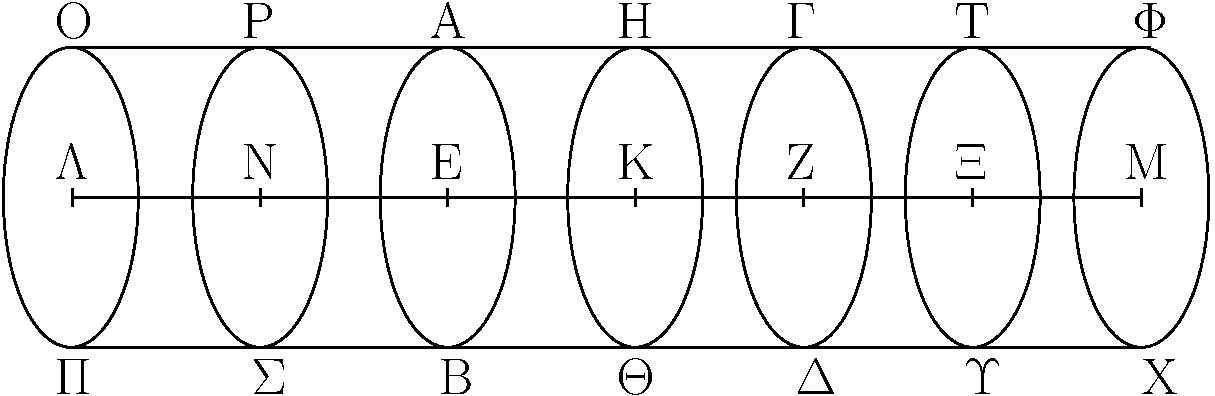
\includegraphics{Book12/fig13g.pdf}}

\gr{Κύλινδροξ γὰρ ὁ ΑΔ ἐπιπέδῳ τῶ| ΗΘ τετμ\kern -.7pt  ήσθω παραλλήλῳ >όντι τοῖξ ἀπεναντίον ἐπιπέδοιξ τοῖξ
ΑΒ, ΓΔ, καὶ συμβαλλέτω τῶ| >άχονι τὸ ΗΘ ἐπίπεδον κατὰ τὸ Κ σημεῖον; λέγω, <ότι ἐστὶν ὡξ ὁ ΒΗ
κύλινδροξ πρὸξ τὸν ΗΔ κύλινδρον, ο<ύτωξ ὁ ΕΚ >άχων πρὸξ τὸν ΚΖ >άχονα.}

\gr{Ἐκβεβλήσθω γὰρ ὁ ΕΖ >άχων ἐφ> ἑκάτερα τὰ μέρη ἐπὶ τὰ Λ, Μ 
σημεῖα, καὶ ἐκκείσθωσαν τῶ|
ΕΚ >άχονι >ίσοι ὁσοιδηποτοῦν οἱ ΕΝ, ΝΛ, τῶ| δὲ ΖΚ >ίσοι ὁσοιδηποτοῦν 
οἱ ΖΧ, ΧΜ, καὶ νοείσθω ὁ ἐπὶ τοῦ ΛΜ >άχονοξ κύλινδροξ ὁ ΟΘ, ο<ῦ
βάσειξ οἱ ΟΠ, ΦΘ κύκλοι. καὶ ἐκβεβλήσθω διὰ τῶν Ν, Χ σημείων ἐπίπεδα παράλληλα τοῖξ ΑΒ, ΓΔ
καὶ ταῖξ βάσεσι τοῦ ΟΘ κυλίνδρου καὶ ποιείτωσαν τοὺξ ΡΣ, ΤΥ κύκλουξ περὶ τὰ Ν, Χ κέντρα.
καὶ ἐπεὶ οἱ ΛΝ, ΝΕ, ΕΚ >άχονεξ >ίσοι εἰσὶν ἀλλήλοιξ, οἱ >άρα ΠΡ, ΡΒ, ΒΗ κύλινδροι
πρὸξ ἀλλήλουξ εἰσὶν ὡξ αἱ βάσειξ. >ίσαι δέ εἰσιν αἱ βάσειξ; >ίσοι >άρα καὶ οἱ ΠΡ, ΡΒ, ΒΗ
κύλινδροι ἀλλήλοιξ. επεὶ ο>ῦν οἱ ΛΝ, ΝΕ, ΕΚ >άχονεξ >ίσοι εἰσὶν ἀλλήλοιξ, εἰσὶ δὲ καὶ
οἱ ΠΡ, ΡΒ, ΒΗ κύλινδροι >ίσοι ἀλλήλοιξ, καί ἐστιν >ίσον τὸ πλῆθοξ τῶ| πλήθει, ὁσαπλασίων
>άρα ὁ ΚΛ >άχων τοῦ ΕΚ >άχονοξ, τοσαυταπλασίων >έσται καὶ ὁ ΠΗ κύλινδροξ τοῦ ΗΒ κυλίνδρου.
διὰ τὰ α\kern -.7pt  ὐτὰ δὴ καὶ ὁσαπλασίων ἐστὶν ὁ ΜΚ >άχων τοῦ ΚΖ >άχονοξ, τοσαυταπλασίων
ἐστὶ καὶ ὁ ΘΗ κύλινδροξ τοῦ ΗΔ κυλίνδρου. καὶ εἰ μὲν >ίσοξ ἐστὶν ὁ ΚΛ >άχων τῶ|
ΚΜ >άχονι, >ίσοξ >έσται καὶ ὁ ΠΗ κύλινδροξ τῶ| ΗΘ κυλίνδρῳ, εἰ δὲ μείζων ὁ
>άχων τοῦ >άχονοξ, μείζων καὶ ὁ κύλινδροξ τοῦ κυλίνδρου, καὶ εἰ ἐλάσσων, ἐλάσσων. τεσσάρων
δὴ μεγεθῶν >όντων, ἀχόνων μὲν τῶν ΕΚ, ΚΖ, κυλίνδρων δὲ τῶν ΒΗ, ΗΔ, ε>ίληπται ἰσάκιξ
πολλαπλάσια, τοῦ μὲν ΕΚ >άχονοξ καὶ τοῦ ΒΗ κυλίνδρου <ό τε ΛΚ >άχων καὶ ὁ ΠΗ κύλινδροξ, τοῦ
δὲ ΚΖ >άχονεξ
καὶ τοῦ ΗΔ κυλίνδρου <ό τε ΚΜ >άχων καὶ ὁ ΗΘ κύλινδροξ,
 καὶ δέδεικται, <ότι εἰ ὑπερέθει ὁ ΚΛ >άχων 
 τοῦ ΚΜ >άχονοξ,
ὑπερέθει καὶ ὁ ΠΗ κύλινδροξ τοῦ ΗΘ κυλίνδρου, καὶ εἰ >ίσοξ, >ίσοξ, καὶ εἰ ἐλάσσων, ἐλάσσων.
>έστιν >άρα ὡξ ὁ ΕΚ >άχων πρὸξ τὸν ΚΖ >άχονα, ο<ύτωξ ὁ ΒΗ
κύλινδροξ πρὸξ τὸν ΗΔ κύλινδρον; <όπερ >έδει δεῖχαι.}}

\ParallelRText{
\begin{center}
{\large Proposition 13}
\end{center}

If a cylinder is cut by a plane which is parallel to the opposite planes (of the cylinder) then
as the cylinder (is) to the cylinder, so the axis will be to the axis.

% Removed epsf size command
\centerline{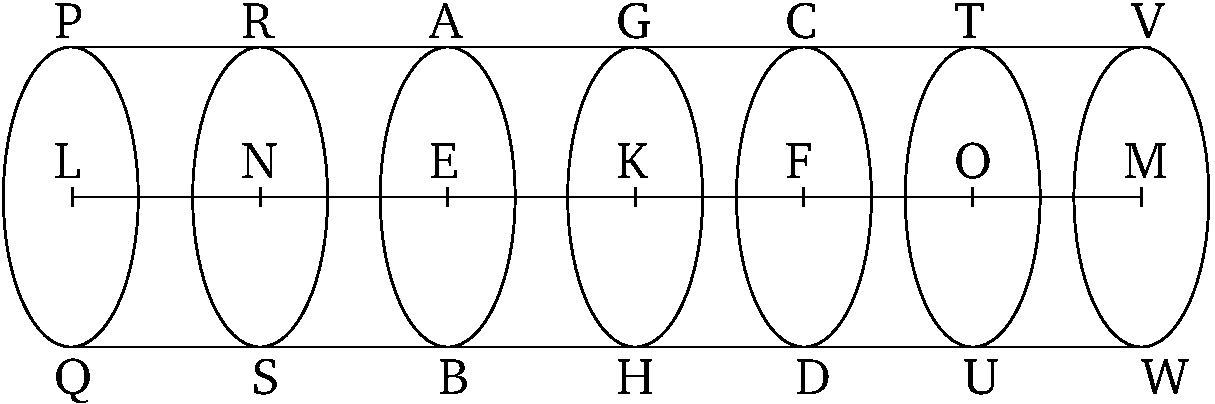
\includegraphics{Book12/fig13e.pdf}}

For let the cylinder $AD$ be cut by the plane $GH$ which is parallel to the opposite planes (of the cylinder), $AB$
and $CD$. And let the plane $GH$ have met the axis at point $K$. I say that as cylinder $BG$
is to cylinder $GD$, so axis $EK$ (is) to axis $KF$.

For let axis $EF$ be produced in each direction to points $L$ and $M$. And let any number whatsoever (of
lengths), $EN$ and $NL$, equal to axis $EK$, be set out (on the axis $EL$), and any number whatsoever
(of lengths), $FO$ and $OM$, equal to (axis) $FK$, (on the axis $KM$). And let the cylinder $PW$, whose bases
(are) the circles $PQ$ and $VW$, be
conceived on axis $LM$. And let planes parallel to $AB$, $CD$, and the bases of cylinder $PW$, be produced
through points $N$ and $O$, and let them have made the circles $RS$ and $TU$ around the centers $N$ and $O$ (respectively).
And since axes $LN$, $NE$, and $EK$ are equal to one another,  the cylinders $QR$, $RB$, and $BG$ are to one another
as their bases [Prop.~12.11]. But the bases are equal. Thus, the cylinders $QR$, $RB$, and $BG$
(are) also equal to one another. Therefore, since the axes $LN$, $NE$, and $EK$ are equal to one another, and the cylinders
$QR$, $RB$, and $BG$ are also equal to one another, and the number (of the former) is equal to the number (of the latter), 
thus as many multiples as axis $KL$ is of axis $EK$, so many multiples is cylinder $QG$ also of cylinder $GB$.
And so, for the same (reasons),  as many multiples as axis $MK$  is of axis $KF$, so many multiples is cylinder $WG$
also of cylinder $GD$.  And if axis $KL$ is equal to axis $KM$ then cylinder $QG$ will also be equal to
cylinder $GW$, and if the axis (is) greater than the axis then the cylinder (will also be) greater than the cylinder, and if (the axis is) less
then (the cylinder will also be) less. So, there are four magnitudes---the axes $EK$ and $KF$, and the cylinders
$BG$ and $GD$---and equal multiples be taken of axis $EK$ and 
cylinder $BG$---(namely), axis $LK$ and
cylinder $QG$---and of axis $KF$
 and  cylinder $GD$---(namely), axis
$KM$ and  cylinder $GW$. And it has been shown that if axis $KL$ exceeds axis $KM$ then cylinder
$QG$ also exceeds  cylinder $GW$, and if (the axes are) equal then (the cylinders are) equal, and if ($KL$ is) less then ($QG$ is) less.
Thus, as axis $EK$ is to axis $KF$, so cylinder $BG$ (is) to cylinder $GD$ [Def.~5.5]. (Which is)
the very thing it was required to show.}
\end{Parallel}

%%%%
%12.14
%%%%
\pdfbookmark[1]{Proposition 12.14}{pdf12.14}
\begin{Parallel}{}{}
\ParallelLText{
\begin{center}
{\large \ggn{14}.}
\end{center}\vspace*{-7pt}

\gr{Οἱ ἐπὶ >ίσων βάσεων >όντεξ κῶνοι καὶ κύλινδροι πρὸξ αλλήλουξ εἰσὶν ὡξ τὰ <ύψη.}

% Removed epsf size command
\centerline{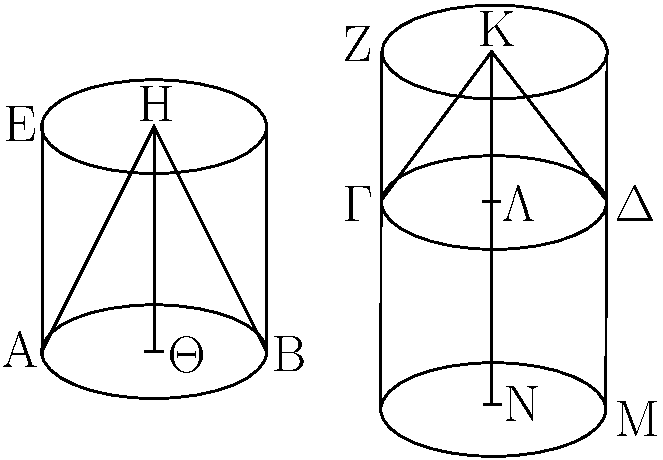
\includegraphics{Book12/fig14g.pdf}}

\gr{>'Εστωσαν γὰρ ἐπὶ >ίσων βάσεων τῶν ΑΒ, ΓΔ κύκλων κύλινδροι οἱ ΕΒ, ΖΔ; λέγω, <ότι
ἐστὶν ὡξ ὁ ΕΒ κύλινδροξ πρὸξ τὸν ΖΔ κύλινδρον, ο<ύτωξ ὁ ΗΘ >άχων πρὸξ τὸν ΚΛ >άχονα.}

\gr{Ἐκβεβλήσθω γὰρ ὁ ΚΛ >άχων ἐπὶ τὸ Ν σημεῖον, καὶ κείσθω τῶ| ΗΘ >άχονι >ίσοξ ὁ ΛΝ,
καὶ περὶ >άχονα τὸν ΛΝ κύλινδροξ νενοήσθω ὁ ΓΜ. ἐπεὶ ο>ῦν οἱ ΕΒ, ΓΜ κύλινδροι
ὑπὸ τὸ α\kern -.7pt  ὐτὸ <ύψοξ εἰσίν, πρὸξ ἀλλήλουξ εἰσὶν ὡξ αἱ βάσειξ. >ίσαι δέ εἰσίν αἱ
βάσειξ ἀλλήλαιξ; >ίσοι >άρα εἰσὶ καὶ οἱ ΕΒ, ΓΜ κύλινδροι. καὶ ἐπεὶ κύλινδροξ ὁ ΖΜ ἐπιπέδῳ
τέτμ\kern -.7pt  ηται τῶ| ΓΔ παραλλήλῳ >όντι τοῖξ ἀπεναντίον ἐπιπέδοιξ, >έστιν >άρα ὡξ ὁ ΓΜ κύλινδροξ
πρὸξ τὸν ΖΔ κύλινδρον, ο<ύτωξ ὁ ΛΝ >άχων πρὸξ τὸν ΚΛ >άχονα. 
>ίσοξ δέ ἐστιν ὁ μὲν ΓΜ  κύλινδροξ τῶ| ΕΒ κυλίνδρῳ, ὁ δὲ ΛΝ >άχων τῶ| ΗΘ >άχονι; >έστιν
>άρα ὡξ ὁ ΕΒ κύλινδροξ πρὸξ τὸν ΖΔ
κύλινδρον, ο<ύτωξ ὁ ΗΘ >άχων πρὸξ τὸν ΚΛ >άχονα. ὡξ δὲ ὁ ΕΒ κύλινδροξ πρὸξ τὸν ΖΔ
κύλινδρον, οὑτωξ ὁ ΑΒΗ κῶνοξ πρὸξ τὸν ΓΔΚ κῶνον. καὶ ὡξ >άρα ὁ ΗΘ >άχων
πρὸξ τὸν ΚΛ >άχονα, ο<ύτωξ ὁ ΑΒΗ κῶνοξ πρὸξ τὸν ΓΔΚ κῶνον καὶ ὁ ΕΒ κύλινδροξ
πρὸξ τὸν ΖΔ κύλινδρον; <όπερ >έδει δεῖχαι.}}

\ParallelRText{
\begin{center}
{\large Proposition 14}
\end{center}

Cones and cylinders which are on equal bases are to one another as their heights.

% Removed epsf size command
\centerline{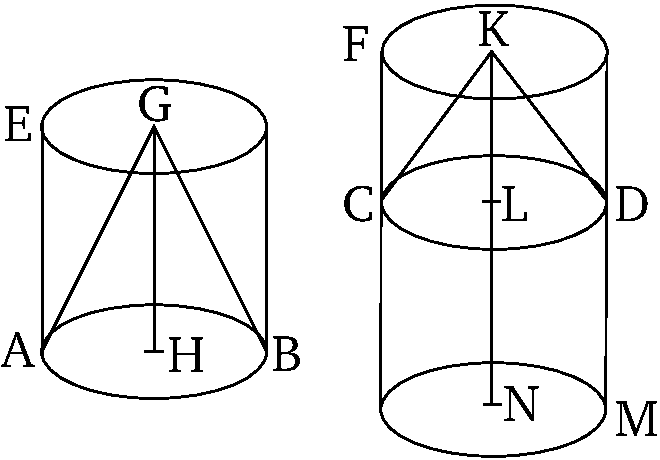
\includegraphics{Book12/fig14e.pdf}}

For let  $EB$ and $FD$ be cylinders on  equal bases, (namely) the circles $AB$ and $CD$ (respectively). I say that as cylinder $EB$
is to cylinder $FD$, so axis $GH$ (is) to axis $KL$.

For let the axis $KL$ be produced to point $N$. And let $LN$ be made equal to axis $GH$. 
And let the cylinder $CM$ be conceived about axis $LN$. Therefore, since cylinders $EB$ and $CM$
have the same height they are to one another as their bases [Prop.~12.11]. And the bases are
equal to one another. Thus, cylinders $EB$ and $CM$ are also equal to one another. And since cylinder $FM$ has been cut
by the plane $CD$, which is parallel to its opposite planes, thus as cylinder $CM$ is to cylinder $FD$, so
axis $LN$ (is) to axis $KL$ [Prop.~12.13]. And cylinder $CM$ is equal to cylinder $EB$, and
axis $LN$ to axis $GH$.  Thus, as cylinder $EB$ is to cylinder $FD$, so axis $GH$ (is) to axis $KL$.  And as
cylinder $EB$ (is) to cylinder $FD$, so cone $ABG$ (is) to cone $CDK$ [Prop.~12.10].
Thus, also, as axis $GH$ (is) to axis $KL$, so cone $ABG$ (is) to cone $CDK$, and cylinder $EB$ to cylinder $FD$.
(Which is) the very thing it was required to show.}
\end{Parallel}

%%%%
%12.15
%%%%
\pdfbookmark[1]{Proposition 12.15}{pdf12.15}
\begin{Parallel}{}{}
\ParallelLText{
\begin{center}
{\large \ggn{15}.}
\end{center}\vspace*{-7pt}

\gr{Τῶν >ίσων κώνων καὶ κυλίνδρων ἀντιπεπόνθασιν αἱ βάσειξ τοῖξ <ύψεσιν; καὶ <ῶν κώνων καὶ
κυλίνδρων ἀντιπεπόνθασιν αἱ βάσειξ τοῖξ <ύψεσιν, >ίσοι εἰσὶν ἐκεῖνοι.}\\

% Removed epsf size command
\centerline{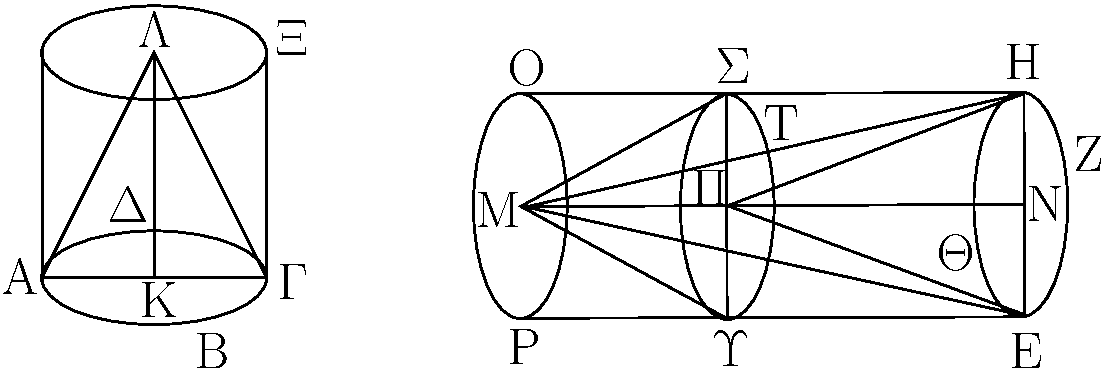
\includegraphics{Book12/fig15g.pdf}}

\gr{>'Εστωσαν >ίσοι κῶνοι καὶ κύλινδροι, <ῶν βάσειξ μὲν οἱ ΑΒΓΔ, ΕΖΗΘ κύκλοι, διάμετροι δὲ
α\kern -.7pt  ὐτῶν αἱ ΑΓ, ΕΗ, <άχονεξ δὲ οἱ ΚΛ, ΜΝ, ο<ίτινεξ καὶ <ύψη εἰσὶ τῶν κώνων >ὴ κυλίνδρων, καὶ
συμπεπληρώσθωσαν οἱ ΑΧ, ΕΟ κύλινδροι. λέγω, <ότι τῶν ΑΧ, ΕΟ κυλίνδρων ἀντιπεπόνθασιν αἱ
βάσειξ τοῖξ <ύψεσιν, καί ἐστιν ὡξ ἡ ΑΒΓΔ βάσιξ πρὸξ τὴν ΕΖΗΘ βάσιν,
ο<ύτωξ τὸ ΜΝ <ύψοξ πρὸξ τὸ ΚΛ <ύψοξ.}

\gr{Τὸ γὰρ ΛΚ <ύψοξ τῶ| ΜΝ <ύψει >ήτοι >ίσον ἐστὶν >ὴ ο>ύ. >έστω πρότερον >ίσον. >έστι δὲ καὶ
ὁ ΑΧ κύλινδροξ τῶ| ΕΟ κυλίνδρῳ >ίσοξ. οἱ δὲ ὑπὸ τὸ α\kern -.7pt  ὐτὸ <ύψοξ >όντεξ κῶνοι καὶ κύλινδροι
πρὸξ ἀλλήλουξ εἰσὶν ὡξ αἱ βάσειξ; >ίση >άρα καὶ ἡ ΑΒΓΔ βάσιξ τῆ| 
ΕΖΗΘ βάσει. <ώστε
καὶ ἀντιπέπονθεν, ὡξ ἡ ΑΒΓΔ βάσιξ πρὸξ τὴν ΕΖΗΘ βάσιν, ο<ύτωξ τὸ ΜΝ <ύψοξ πρὸξ τὸ
ΚΛ <ύψοξ. ἀλλὰ δὴ μ\kern -.7pt  ὴ >έστω τὸ ΛΚ <ύψοξ τῶ| ΜΝ >ίσον, ἀλλ> >έστω μεῖζον τὸ ΜΝ, 
καὶ ἀφῃρήσθω ἀπὸ τοῦ ΜΝ <ύψουξ τῶ| ΚΛ >ίσον τὸ ΠΝ, καὶ διὰ τοῦ Π σημείου τετμ\kern -.5pt  ήσθω ὁ
ΕΟ κύλινδροξ ἐπιπέδῳ τῶ| ΤΥΣ παραλλήλῳ τοῖξ τῶν ΕΖΗΘ, ΡΟ κύκλων ἐπιπέδοιξ,
καὶ ἀπὸ βάσεωξ μὲν τοῦ ΕΖΗΘ κύκλου, <ύψουξ δὲ τοῦ ΝΠ κύλινδροξ νενοήσθω ὁ ΕΣ. καί
ἐπεὶ >ίσοξ ἐστὶν ὁ ΑΧ κύλινδροξ τῶ| ΕΟ κυλίνδρῳ, >έστιν >άρα ὡξ ὁ ΑΧ κύλινδροξ
πρὸξ τὸν ΕΣ κυλίνδρον, ο<ύτωξ ὁ ΕΟ κύλινδροξ πρὸξ τὸν ΕΣ κύλινδρον.
 ἀλλ> ὡξ μὲν ὁ ΑΧ κύλινδροξ πρὸξ τὸν ΕΣ κύλινδρον,
ο<ύτωξ ἡ ΑΒΓΔ βάσιξ πρὸξ τὴν ΕΖΗΘ; ὑπὸ γὰρ τὸ  α\kern -.3pt  ὐτὸ <ύψοξ εἰσὶν οἱ ΑΧ, ΕΣ κύλινδροι; ὡξ
δὲ ὁ ΕΟ κύλινδροξ πρὸξ  τὸν ΕΣ, ο<ύτωξ τὸ ΜΝ  <ύψοξ πρὸξ τὸ ΠΝ <ύψοξ; ὁ γὰρ ΕΟ κύλινδροξ ἐπιπέδῳ
τέτμ\kern -.7pt  ηται παραλλήλῳ >όντι τοῖξ ἀπεναντίον ἐπιπέδοιξ.  >έστιν >άρα καὶ ὡξ ἡ ΑΒΓΔ βάσιξ πρὸξ τὴν ΕΖΗΘ βάσιν, ο<ύτωξ τὸ ΜΝ <ύψοξ πρὸξ τὸ ΠΝ
<ύψοξ. >ίσον δὲ τὸ ΠΝ <ύψοξ τῶ| ΚΛ <ύψει; >έστιν >άρα ὡξ ἡ  ΑΒΓΔ βάσιξ πρὸξ τὴν ΕΖΗΘ
βάσιν, ο<ύτωξ τὸ ΜΝ <ύψοξ πρὸξ τὸ ΚΛ <ύψοξ. τῶν >άρα ΑΧ, ΕΟ κυλίνδρων ἀντιπεπόνθασιν αἱ
βάσειξ τοῖξ <ύψεσιν.}

\gr{Ἀλλὰ δὴ τῶν ΑΧ, ΕΟ κυλίνδρων ἀντιπεπονθέτωσαν αἱ βάσειξ τοῖξ <ύψεσιν, καὶ >έστω ὡξ ἡ ΑΒΓΔ
βάσιξ πρὸξ τὴν ΕΖΗΘ βάσιν, ο<ύτωξ τὸ ΜΝ <ύψοξ πρὸξ τὸ ΚΛ <ύψοξ; λέγω, <ότι >ίσοξ ἐστὶν
ὁ ΑΧ κύλινδροξ τῶ| ΕΟ κυλίνδρῳ.}

\gr{Τῶν γὰρ α\kern -.7pt  ὐτῶν κατασκευασθέντων ἐπεί ἐστιν ὡξ ἡ ΑΒΓΔ βάσιξ πρὸξ τὴν ΕΖΗΘ βάσιν, ο<ύτωξ
τὸ ΜΝ <ύψοξ πρὸξ τὸ ΚΛ <ύψοξ, >ίσον δὲ τὸ ΚΛ <ύψοξ τῶ| ΠΝ <ύψει, >έσται >άρα ὡξ ἡ ΑΒΓΔ βάσιξ
πρὸξ τὴν ΕΖΗΘ βάσιν, ο<ύτωξ τὸ ΜΝ <ύψοξ πρὸξ τὸ ΠΝ <ύψοξ. ἀλλ> ὡξ μὲν ἡ ΑΒΓΔ βάσιξ
πρὸξ τὴν ΕΖΗΘ βάσιν, ο<ύτωξ ὁ ΑΧ κύλινδροξ πρὸξ τὸν ΕΣ κύλινδρον; ὑπὸ γὰρ τὸ α\kern -.7pt  ὐτὸ
<ύψοξ εἰσίν; ὡξ δὲ τὸ ΜΝ <ύψοξ πρὸξ τὸ ΠΝ [<ύψοξ], ο<ύτωξ ὁ ΕΟ κύλινδροξ πρὸξ τὸν
ΕΣ κύλινδρον; >έστιν >άρα ὡξ ὁ ΑΧ κύλινδροξ πρὸξ τὸν ΕΣ κύλινδρον, ο<ύτωξ ὁ ΕΟ
κύλινδροξ πρὸξ τὸν ΕΣ. >ίσοξ >άρα ὁ ΑΧ κύλινδροξ τῶ| ΕΟ κυλίνδρῳ. ὡσαύτωξ δὲ καὶ ἐπὶ τῶν κώνων;
<όπερ >έδει δεῖχαι.}}

\ParallelRText{
\begin{center}
{\large Proposition 15}
\end{center}

The bases of equal cones and cylinders are reciprocally proportional to their heights. And, those
cones and cylinders whose bases (are) reciprocally proportional to their heights are equal.

% Removed epsf size command
\centerline{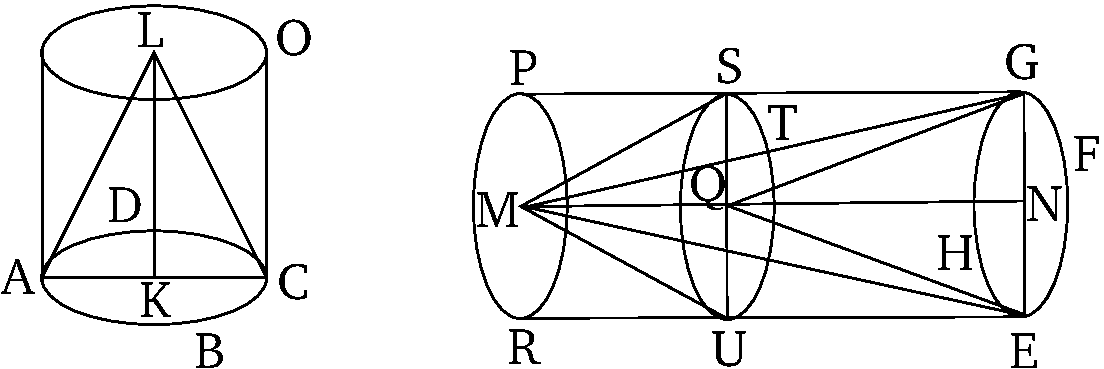
\includegraphics{Book12/fig15e.pdf}}

Let there be equal cones and cylinders whose bases are the circles $ABCD$ and $EFGH$, and  the diameters of (the bases) $AC$ and $EG$, and
(whose) axes (are) $KL$ and $MN$, which are also the heights of the cones and cylinders (respectively).
And let the cylinders $AO$ and $EP$ 
be completed. I say that the bases of cylinders $AO$  and $EP$ are reciprocally proportional to their heights, and (so) as base
$ABCD$ is to base $EFGH$, so height $MN$ (is) to height $KL$.

For height $LK$ is either equal to height $MN$, or not. Let it, first of all, be equal. And cylinder $AO$ is also equal to cylinder $EP$.
And cones and cylinders having the same height are to one another as their bases [Prop.~12.11]. 
Thus, base $ABCD$ (is) also equal to base $EFGH$. And, hence, reciprocally, as base $ABCD$ (is) to base $EFGH$,
so height $MN$ (is) to height $KL$. And so, let height $LK$ not be equal to $MN$, but let $MN$ be greater. And let $QN$, equal to
$KL$, be cut off from height $MN$. And let the cylinder $EP$ be cut, through point $Q$, by the plane $TUS$ (which is)
parallel to the planes of the circles $EFGH$ and $RP$. And let cylinder $ES$ be conceived, with base the circle $EFGH$, and
height $NQ$. And since cylinder $AO$ is equal to cylinder $EP$, thus, as cylinder $AO$ (is) to cylinder $ES$, so cylinder
$EP$ (is) to cylinder $ES$ [Prop.~5.7]. But, as cylinder $AO$ (is) to cylinder $ES$, so base $ABCD$ (is)
to base $EFGH$. For cylinders $AO$ and $ES$ (have)  the same height [Prop.~12.11]. 
And as cylinder $EP$ (is) to (cylinder) $ES$, so height $MN$ (is) to height  $QN$. For cylinder $EP$
has been cut by a plane which is parallel to its opposite planes [Prop.~12.13].
And, thus, as base $ABCD$ is to base $EFGH$, so height $MN$ (is) to height $QN$ [Prop.~5.11]. And height $QN$
(is) equal to height $KL$. Thus, as base $ABCD$ is to base $EFGH$, so height $MN$ (is) to height $KL$.
Thus, the bases of cylinders $AO$ and $EP$ are reciprocally proportional to their heights.

And, so, let the bases of cylinders $AO$ and $EP$ be reciprocally proportional to their heights, and (thus) let
base $ABCD$ be to base $EFGH$, as height $MN$ (is) to height $KL$. I say that cylinder $AO$ is equal to
cylinder $EP$.

For, with the same construction, since  as base $ABCD$ is to base $EFGH$, so  height $MN$ (is) to height $KL$, and
height $KL$ (is) equal to height $QN$, thus, as base $ABCD$ (is) to base $EFGH$, so height $MN$ will be to height $QN$.
But, as base $ABCD$ (is) to base $EFGH$, so cylinder $AO$ (is) to cylinder $ES$. For they are the same height [Prop.~12.11]. 
And as height $MN$ (is) to [height] $QN$, so cylinder $EP$ (is) to cylinder $ES$ [Prop.~12.13].
Thus, as cylinder $AO$ is to cylinder $ES$, so cylinder $EP$ (is) to (cylinder) $ES$ [Prop.~5.11]. Thus, cylinder $AO$ (is)
equal to cylinder $EP$ [Prop.~5.9]. In the same manner, (the proposition can) also (be demonstrated)
for the cones. (Which is) the very thing it was required to show.}
\end{Parallel}

%%%%
%12.16
%%%%
\pdfbookmark[1]{Proposition 12.16}{pdf12.16}
\begin{Parallel}{}{}
\ParallelLText{
\begin{center}
{\large \ggn{16}.}
\end{center}\vspace*{-7pt}

\gr{Δύο κύκλων περὶ τὸ α\kern -.7pt  ὐτὸ κέντρον >όντων εἰξ τὸν μείζονα κύκλον πολύγωνον ἰσόπλευρόν τε καὶ ἀρτιόπλευ\-ρον
ἐγγράψαι μ\kern -.7pt  ὴ ψα\kern -.5pt  ῦον τοῦ ἐλάσσονοξ κύκλου.}

% Removed epsf size command
\centerline{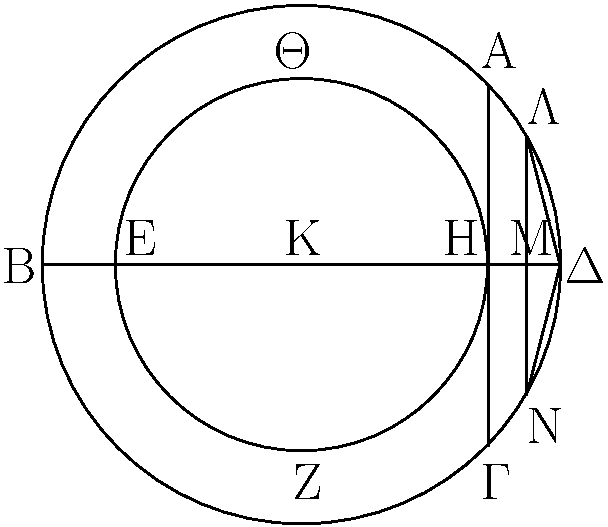
\includegraphics{Book12/fig16g.pdf}}

\gr{>'Εστωσαν οἱ δοθέντεξ δύο κύκλοι οἱ ΑΒΓΔ, ΕΖΗΘ περὶ τὸ α\kern -.7pt  ὐτὸ κέντρον τὸ Κ; δεῖ δὴ εἰξ τὸν μείζονα κύκλον τὸν ΑΒΓΔ πολύγωνον ἰσόπλευρόν τε καὶ ἀρτιόπλευρον ἐγγράψαι μ\kern -.7pt  ὴ ψα\kern -.5pt  ῦον τοῦ ΕΖΗΘ κύκλου.}

\gr{>'Ηθθω γὰρ διὰ τοῦ Κ κέντρου εὐθεῖα ἡ ΒΚΔ, καὶ ἀπὸ τοῦ Η σημείου τῆ| ΒΔ εὐθείᾳ πρὸξ ὀρθὰξ
>ήθθω ἡ ΗΑ καὶ διήθθω ἐπὶ τὸ Γ; ἡ ΑΓ >άρα ἐφάπτεται τοῦ ΕΖΗΘ κύκλου. τέμνοντεξ δὴ τὴν ΒΑΔ περιφέρειαν
δίθα καὶ τὴν ἡμίσειαν α\kern -.7pt  ὐτῆξ δίθα καὶ τοῦτο ἀεὶ ποιοῦντεξ καταλείψομεν περιφέρειαν ἐλάσσονα
τῆξ ΑΔ. λελείφθω, καὶ >έστω ἡ ΛΔ, καὶ ἀπὸ τοῦ Λ ἐπὶ τὴν ΒΔ
κάθετοξ >ήθθω ἡ ΛΜ καὶ
διήθθω ἐπὶ τὸ Ν, καὶ ἐπεζεύθθωσαν αἱ ΛΔ, ΔΝ; >ίση
>άρα ἐστὶν ἡ ΛΔ τῆ| ΔΝ. καὶ ἐπεὶ παράλληλόξ ἐστιν ἡ ΛΝ τῆ| ΑΓ, 
ἡ δὲ ΑΓ ἐφάπτεται τοῦ ΕΖΗΘ κύκλου, ἡ ΛΝ >άρα
οὐκ ἐφάπτεται τοῦ ΕΖΗΘ κύκλου; πολλῶ| >άρα αἱ ΛΔ, ΔΝ οὐκ ἐφάπτονται τοῦ ΕΖΗΘ κύκλου. ἒαν δὴ τῆ| ΛΔ
εὐθείᾳ >ίσαξ κατὰ τὸ συνεθὲξ ἐναρμόσωμεν εἰξ τὸν ΑΒΓΔ κύκλον, ἐγγραφήσεται εἰξ τὸν ΑΒΓΔ κύκλον
πολύγωνον ἰσόπλευρόν τε καὶ ἀρτιόπλευρον μ\kern -.7pt  ὴ ψα\kern -.5pt  ῦον τοῦ ἐλάσσονοξ κύκλου τοῦ ΕΖΗΘ; <όπερ >έδει ποιῆσαι.}}

\ParallelRText{
\begin{center}
{\large Proposition 16}
\end{center}

There being two circles about the same center, to inscribe an equilateral and even-sided polygon in the
greater circle, not touching the lesser circle.

% Removed epsf size command
\centerline{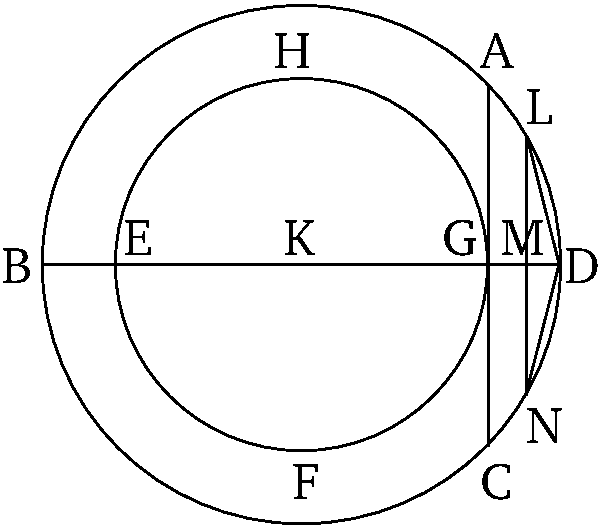
\includegraphics{Book12/fig16e.pdf}}

Let $ABCD$ and $EFGH$ be the given two circles, about the same center, $K$. So, it is necessary
to inscribe an equilateral and even-sided polygon in the greater circle $ABCD$, not touching circle $EFGH$.

Let the straight-line $BKD$ be drawn through the center $K$. And let $GA$ be drawn, at right-angles to the
straight-line $BD$, through point $G$, and let it be drawn through to $C$. Thus, $AC$ touches  circle $EFGH$ [Prop.~3.16~corr.]. 
So, (by) cutting circumference $BAD$ in half, and the half of it in half, and 
doing this continually, we will (eventually) leave
a circumference less than $AD$ [Prop.~10.1]. Let it be left, and let it be $LD$. And let $LM$ be drawn, from $L$, 
perpendicular to $BD$, and let it be drawn through to $N$. And let $LD$ and $DN$ be joined. 
Thus, $LD$ is equal to $DN$ [Props.~3.3, 1.4]. 
And since $LN$ is
parallel to $AC$ [Prop.~1.28], and $AC$ touches circle $EFGH$, $LN$ thus does not touch circle $EFGH$. Thus,
even more so, $LD$ and $DN$ do not touch circle $EFGH$. And if we continuously insert (straight-lines) equal to straight-line
$LD$ into circle $ABCD$ [Prop.~4.1] then an equilateral and even-sided polygon, not touching
the lesser circle $EFGH$, will be inscribed in circle $ABCD$.$^\dag$ (Which is) the very thing it was required to do.}
\end{Parallel}
{\footnotesize\noindent$^\dag$ Note that the chord of the polygon, $LN$, does not touch the inner circle either.}

%%%%
%12.17
%%%%
\pdfbookmark[1]{Proposition 12.17}{pdf12.17}
\begin{Parallel}{}{}
\ParallelLText{
\begin{center}
{\large \ggn{17}.}
\end{center}\vspace*{-7pt}

\gr{Δύο σφαιρῶν περὶ τὸ α\kern -.7pt  ὐτὸ κέντρον οὐσῶν εἰξ τὴν μείζονα σφαῖραν στερεὸν πολύεδρον ἐγγράψαι μ\kern -.7pt  ὴ ψα\kern -.5pt  ῦον
τῆξ ἐλάσσονοξ σφαίραξ κατὰ τὴν ἐπιφάνειαν.}

% Removed epsf size command
\centerline{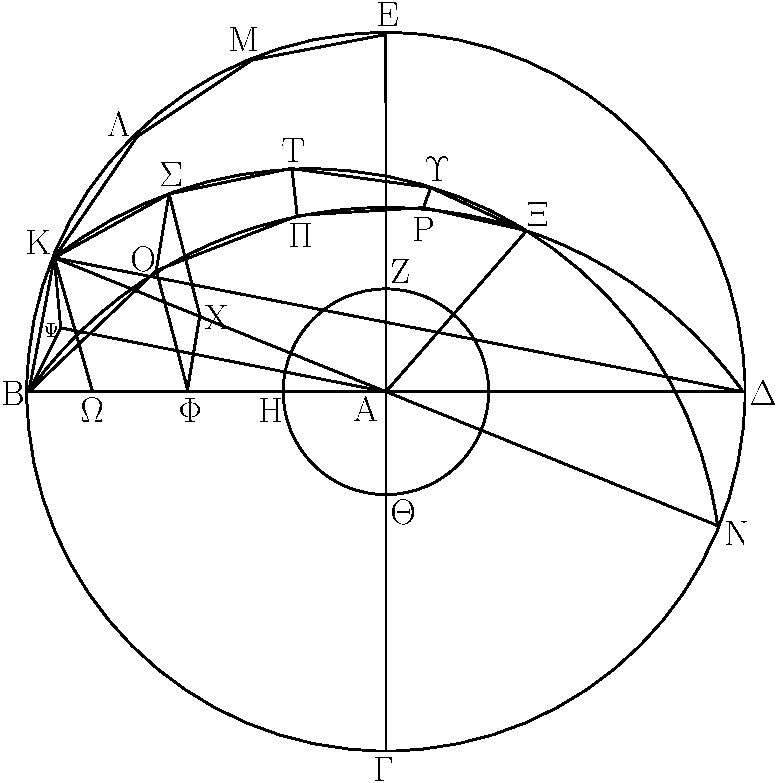
\includegraphics{Book12/fig17g.pdf}}

\gr{Νενοήσθωσαν δύο σφαῖραι περὶ τὸ α\kern -.7pt  ὐτὸ κέντρον τὸ Α; δεῖ δὴ εἰξ τὴν μείζονα σφαῖραν στερεὸν πολύεδρον
ἐγγράψαι μ\kern -.7pt  ὴ ψα\kern -.5pt  ῦον τῆξ ἐλάσσονοξ σφαίραξ κατὰ τὴν ἐπιφάνειαν.}

\gr{Τετμ\kern -.7pt  ήσθωσαν αἱ σφαῖραι ἐπιπέδῳ τινὶ διὰ τοῦ κέντρου; >έσονται δὴ αἱ τομαὶ κύκλοι,
ἐπειδήπερ μενούσηξ τῆξ διαμέτρου καὶ περιφερομένου τοῦ ἡμικυκλίου ἐγιγνετο ἡ σφαῖρα; <ώστε καὶ καθ>
ο<ίαξ >ὰν θέσεωξ ἐπινοήσωμεν τὸ ἡμικύκλιον, τὸ δι> α\kern -.7pt  ὐτοῦ ἐκβαλλόμενον ἐπίπεδον ποιήσει ἐπὶ
τῆξ ἐπιφανείαξ τῆξ σφαίραξ κύκλον. καὶ φανερόν, <ότι καὶ μέγιστον, ἐπειδήπερ ἡ διάμετροξ τῆξ
σφαίραξ, <ήτιξ ἐστὶ καὶ τοῦ ἡμικυκλίου διάμετροξ
 δηλαδὴ
καὶ τοῦ κύκλου, μείζων ἐστὶ πασῶν τῶν εἰξ τὸν κύκλον >ὴ τὴν σφαῖραν διαγομένων [εὐθειῶν]. >έστω
ο>ῦν ἐν μὲν τῆ| μείζονι σφαίρᾳ κύκλοξ ὁ ΒΓΔΕ, ἐν δὲ τῆ| ἐλάσσονι σφαίρᾳ κύκλοξ ὁ ΖΗΘ, καὶ >ήθθωσαν α\kern -.5pt  ὐτῶν
δύο διάμετροι πρὸξ ὀρθὰξ ἀλλήλαιξ αἱ ΒΔ, ΓΕ, καὶ δύο κύκλων περὶ τὸ α\kern -.3pt  ὐτὸ κέντρον >όντων τῶν ΒΓΔΕ, ΖΗΘ
εἰξ τὸν μείζονα κύκλον τὸν ΒΓΔΕ πολύγωνον ἰσόπλευρον καὶ ἀρτιόπλευρον ἐγγεγράφθω μ\kern -.7pt  ὴ ψα\kern -.7pt  ῦον
τοῦ ἐλάσσονοξ κύκλου τοῦ ΖΗΘ, ο<ῦ πλευραὶ >έστωσαν ἐν τῶ| ΒΕ  τεταρτημορίῳ αἱ ΒΚ, ΚΛ, ΛΜ, ΜΕ, καὶ
ἐπιζευθθεῖσα ἡ ΚΑ διήθθω ἐπὶ τὸ Ν, καὶ ἀνεστάτω ἀπὸ τοῦ Α σημείου τῶ| τοῦ ΒΓΔΕ κύκλου
ἐπιπέδῳ πρὸξ ὀρθὰξ ἡ ΑΧ καὶ συμβαλλέτω τῆ| ἐπιφανείᾳ τῆξ σφαίραξ κατὰ τὸ Χ, καὶ διὰ τῆξ ΑΧ καὶ ἑκατέραξ
τῶν ΒΔ, ΚΝ ἐπίπεδα ἐκβεβλήσθω; ποιήσουσι δὴ διὰ τὰ εἰρημένα
ἐπὶ τῆξ ἐπιφανείαξ τῆξ σφαίραξ μεγίστουξ κύκλουξ. ποιείτωσαν, <ῶν ἡμικύκλια >έστω ἐπὶ τῶν ΒΔ, ΚΝ
διαμέτρων τὰ ΒΧΔ, ΚΧΝ. καὶ ἐπεὶ ἡ ΧΑ ὀρθή ἐστι πρὸξ τὸ τοῦ ΒΓΔΕ κύκλου ἐπίπεδον, καὶ
πάντα >άρα τὰ διὰ τῆξ ΧΑ ἐπίπεδά ἐστιν ὀρθὰ πρὸξ τὸ τοῦ
ΒΓΔΕ κύκλου ἐπίπεδον; <ώστε καὶ τὰ ΒΧΔ, ΚΧΝ ἡμικύκλια ὀρθά ἐστι πρὸξ τὸ τοῦ ΒΓΔΕ κύκλου ἐπίπεδον.
καὶ ἐπεὶ >ίσα ἐστὶ τὰ ΒΕΔ, ΒΧΔ, ΚΧΝ ἡμικύκλια; ἐπὶ γὰρ >ίσων εἰσὶ διαμέτρων τῶν ΒΔ, ΚΝ; >ίσα
ἐστὶ καὶ τὰ ΒΕ, ΒΧ, ΚΧ τεταρτημόρια ἀλλήλοιξ. >όσαι >άρα εἰσὶν ἐν τῶ| ΒΕ τεταρτημορίῳ
πλευραὶ τοῦ πολυγώνου, τοσα\kern -.7pt  ῦταί εἰσι καὶ ἐν τοῖξ ΒΧ, ΚΧ τεταρτημορίοιξ >ίσαι ταῖξ ΒΚ, ΚΛ, ΛΜ, ΜΕ εὐθείαιξ.
ἐγγεγράφθωσαν καὶ >έστωσαν αἱ ΒΟ, ΟΠ, ΠΡ, ΡΧ, ΚΣ, ΣΤ, ΤΥ, ΥΧ,  καὶ ἐπεζεύθθωσαν αἱ ΣΟ, ΤΠ,
ΥΡ, καὶ ἀπὸ τῶν Ο, Σ ἐπὶ τὸ τοῦ ΒΓΔΕ κύκλου ἐπίπεδον κάθετοι >ήθθωσαν; πεσοῦνται
δὴ ἐπὶ τὰξ κοινὰξ τομὰξ τῶν ἐπιπέδων τὰξ ΒΔ, ΚΝ, ἐπειδήπερ καὶ τὰ τῶν ΒΧΔ, ΚΧΝ ἐπίπεδα ὀρθά
ἐστι πρὸξ τὸ τοῦ ΒΓΔΕ κύκλου ἐπίπεδον. πιπτέτωσαν, καὶ >έστωσαν αἱ ΟΦ, ΣΘ, καὶ ἐπεζεύθθω ἡ ΘΦ.
καὶ ἐπεὶ ἐν >ίσοιξ ἡμικυκλίοιξ τοῖξ ΒΧΔ, ΚΧΝ >ίσαι ἀπειλημμέναι εἰσὶν αἱ ΒΟ, ΚΣ,
καὶ κάθετοι ἠγμέναι εἰσὶν αἱ ΟΦ, ΣΘ, >ίση [>άρα] ἐστὶν ἡ μὲν ΟΦ τῆ| ΣΘ, ἡ δὲ ΒΦ
τῆ| ΚΘ. >έστι δὲ καὶ <όλη ἡ ΒΑ <όλῃ τῆ| ΚΑ >ίση; καὶ λοιπὴ >άρα ἡ ΦΑ λοιπῆ| τῆ| ΘΑ ἐστιν
>ίση; >έστιν >άρα ὡξ ἡ ΒΦ πρὸξ τὴν ΦΑ, ο<ύτωξ ἡ ΚΘ πρὸξ τὴν ΘΑ; παράλληλοξ >άρα ἐστὶν ἡ ΘΦ τῆ| ΚΒ. καὶ
ἐπεὶ ἑκατέρα τῶν ΟΦ, ΣΘ ὀρθή ἐστι πρὸξ τὸ τοῦ ΒΓΔΕ κύκλου ἐπίπεδον, παράλληλοξ >άρα ἐστὶν ἡ ΟΦ τῆ| ΣΘ. ἐδείθθη
δὲ α\kern -.7pt  ὐτῆ| καὶ >ίση; καὶ αἱ ΘΦ, ΣΟ >άρα >ίσαι εἰσὶ καὶ παράλληλοι. καὶ ἐπεὶ παράλληλόξ ἐστιν ἡ ΘΦ τῆ|
ΣΟ, ἀλλὰ ἡ ΘΦ τῆ| ΚΒ ἐστι παράλληλοξ, καὶ ἡ ΣΟ >άρα τῆ| ΚΒ ἐστι παράλληλοξ. καὶ ἐπιζευγνύουσιν
α\kern -.7pt  ὐτὰξ αἱ ΒΟ, ΚΣ; τὸ ΚΒΟΣ >άρα τετράπλευρον ἐν ἑνί ἐστιν ἐπιπέδῳ, ἐπειδήπερ, ἒαν >ῶσι δύο
εὐθεῖαι παράλληλοι, καὶ ἐφ> ἑκατέραξ α\kern -.7pt  ὐτῶν ληφθῆ| τυθόντα σημεῖα, ἡ ἐπὶ τὰ σημεῖα ἐπιζευγνυμένη
εὐθεῖα ἐν τῶ| α\kern -.7pt  ὐτῶ| ἐπιπέδῳ ἐστὶ ταῖξ παραλλήλοιξ. διὰ τὰ α\kern -.7pt  ὐτὰ δὴ καὶ ἑκάτερον τῶν ΣΟΠΤ, ΤΠΡΥ
τετραπλεύρων ἐν ἑνί ἐστιν ἐπιπέδῳ. >έστι δὲ καὶ τὸ ΥΡΧ τρίγωνον ἐν ἑνὶ ἑπιπέδῳ.
ἒαν δὴ νοήσωμεν ἀπὸ τῶν Ο, Σ, Π, Τ, Ρ, Υ σημείων ἐπὶ τὸ Α
ἐπιζευγνυμέναξ εὐθείαξ, συσταθήσεταί τι σθῆμα στερεὸν πολύεδρον ματαχὺ τῶν ΒΧ, ΚΧ περιφερειῶν ἐκ πυραμίδων
συγκείμενον, <ῶν βάσειξ μὲν τὰ ΚΒΟΣ, ΣΟΠΤ, ΤΠΡΥ τετράπλευρα καὶ τὸ ΥΡΧ τρίγωνον, κορυφὴ δὲ τὸ Α σημεῖον. ἒαν
δὲ καὶ ἐπὶ ἑκάστηξ τῶν ΚΛ, ΛΜ, ΜΕ πλευρῶν καθάπερ ἐπὶ τῆξ ΒΚ τὰ α\kern -.7pt  ὐτὰ κατασκευάσωμεν καὶ
>έτι τῶν λοιπῶν τριῶν τεταρτημορίων, συσταθήσεταί τι σθῆμα πολύεδρον ἐγγεγραμμένον εἰξ τὴν σφαῖραν
πυραμίσι περιεχόμενον, <ῶν βάσιεξ [μὲν] τὰ εἰρημένα τετράπλευρα καὶ τὸ ΥΡΧ τρίγωνον καὶ τὰ ὁμοταγῆ
α\kern -.7pt  ὐτοῖξ, κορυφὴ δὲ τὸ Α σημεῖον.}

\gr{Λέγω <ότι τὸ εἰρημένον πολύεδρον οὐκ ἐφάψεται τῆξ ἐλάσσονοξ σφαίραξ κατὰ τὴν ἐπιφάνειαν, ἐφ> <ῆξ
ἐστιν ὁ ΖΗΘ κύκλοξ.}

\gr{>'Ηθθω ἀπὸ τοῦ Α σημείου ἐπὶ τὸ τοῦ ΚΒΟΣ τετραπλεύρου ἐπίπεδον 
κάθετοξ ἡ ΑΨ καὶ συμβαλλέτω
τῶ| ἐπιπέδῳ κατὰ τὸ Ψ σημεῖον, καὶ ἐπεζεύθθωσαν αἱ  ΨΒ, ΨΚ. καὶ ἐπεὶ ἡ ΑΨ ὀρθή ἐστι
πρὸξ τὸ τοῦ ΚΒΟΣ τετραπλεύρου ἐπίπεδον, καὶ πρὸξ πάσαξ >άρα τὰξ ἁπτομέναξ α\kern -.7pt  ὐτῆξ εὐθείαξ
καὶ ο>ύσαξ ἐν τῶ| τοῦ τετραπλεύρου ἐπιπέδῳ ὀρθή ἐστιν. ἡ ΑΨ >άρα ὀρθή ἐστι πρὸξ ἑκατέραν τῶν ΒΨ, ΨΚ.
καὶ ἐπεὶ >ίση ἐστὶν ἡ ΑΒ τῆ| ΑΚ, <ίσον ἐστὶ καὶ τὸ ἀπὸ
τῆξ ΑΒ τῶ| ἀπὸ τῆξ ΑΚ. καί ἐστι τῶ| μὲν ἀπὸ τῆξ ΑΒ >ίσα  τὰ ἀπὸ τῶν ΑΨ, ΨΒ; ὀρθὴ γὰρ ἡ πρὸξ τῶ| Ψ; τῶ| δὲ ἀπὸ τῆξ ΑΚ >ίσα τὰ ἀπὸ τῶν
ΑΨ, ΨΚ. τὰ >άρα ἀπὸ τῶν ΑΨ, ΨΒ >ίσα ἐστὶ τοῖξ ἀπὸ τῶν ΑΨ, ΨΚ. κοινὸν ἀφῃρήσθω τὸ ἀπὸ τῆξ
ΑΨ; λοιπὸν  >άρα τὸ ἀπὸ τῆξ ΒΨ λοιπῶ| τῶ| ἀπὸ τῆξ ΨΚ >ίσον ἐστίν; >ίση >άρα
ἡ ΒΨ τῆ| ΨΚ. ὁμοίωξ δὴ δείχομεν, <ότι καὶ  αἱ ἀπὸ τοῦ Ψ ἐπὶ τὰ Ο, Σ ἐπιζευγνύμεναι
εὐθεῖαι >ίσαι εἰσὶν ἑκατέρᾳ τῶν ΒΨ, ΨΚ. ὁ >άρα κέντρῳ τῶ| Ψ καὶ διαστήματι ἑνὶ τῶν ΨΒ, ΨΚ
γραφόμενοξ κύκλοξ <ήχει καὶ διὰ τῶν Ο, Σ, καὶ >έσται ἐν κύκλῳ τὸ ΚΒΟΣ τετράπλευρον.}

\gr{Καὶ ἐπεὶ μείζων ἐστὶν ἡ ΚΒ τῆξ ΘΦ, >ίση δὲ ἡ ΘΦ τῆ| ΣΟ, μείζων >άρα ἡ ΚΒ τῆξ ΣΟ. >ίση
δὲ ἡ ΚΒ ἑκατέρᾳ τῶν ΚΣ, ΒΟ; καὶ ἑκατέρα >άρα τῶν ΚΣ, ΒΟ τῆξ ΣΟ μείζων ἐστίν. καὶ ἐπεὶ
ἐν κύκλῳ τετράπλευρόν ἐστι τὸ ΚΒΟΣ, καὶ >ίσαι αἱ ΚΒ, ΒΟ, ΚΣ, καὶ ἐλάττων ἡ ΟΣ, καὶ
ἐκ τοῦ κέντρου τοῦ κύκλου ἐστὶν ἡ ΒΨ, τὸ >άρα ἀπὸ τῆξ ΚΒ τοῦ ἀπὸ τῆξ ΒΨ μεῖζόν ἐστιν 	>ὴ διπλάσιον. >ήθθω
ἀπὸ τοῦ Κ ἐπὶ τὴν ΒΦ κάθετοξ ἡ ΚΩ. καὶ ἐπεὶ ἡ ΒΔ τῆξ ΔΩ ἐλάττων ἐστὶν >ὴ διπλῆ, καί ἐστιν ὡξ ἡ ΒΔ πρὸξ
τὴν ΔΩ, ο<ύτωξ τὸ ὑπὸ τῶν ΔΒ, ΒΩ πρὸξ τὸ ὑπὸ [τῶν] ΔΩ, ΩΒ, ἀναγραφομένου ἀπὸ τῆξ ΒΩ τετραγώνου
καὶ συμπληρουμένου τοῦ ἐπὶ τῆξ ΩΔ παραλληλογράμμου καὶ τὸ ὑπὸ ΔΒ, ΒΩ >άρα τοῦ ὑπὸ ΔΩ,
ΩΒ >έλαττόν ἐστιν >ὴ διπλάσιον. καί ἐστι τῆξ ΚΔ
ἐπιζευγνυμένηξ τὸ μὲν ὑπὸ ΔΒ, ΒΩ  >ίσον τῶ| ἀπὸ τῆξ ΒΚ, τὸ δὲ ὑπὸ τῶν ΔΩ, ΩΒ >ίσον τῶ| ἀπὸ
τῆξ ΚΩ; τὸ >άρα ἀπὸ τῆξ ΚΒ τοῦ ἀπὸ τῆξ ΚΩ >έλασσόν ἐστιν >ὴ διπλάσιον. ἀλλὰ τὸ ἀπὸ τῆξ ΚΒ τοῦ
ἀπὸ τῆξ ΒΨ μεῖζόν ἐστιν >ὴ διπλάσιον; μεῖζον >άρα τὸ ἀπὸ τῆξ  ΚΩ τοῦ ἀπὸ τῆξ ΒΨ. καὶ ἐπεὶ
>ίση ἐστὶν ἡ ΒΑ τῆ| ΚΑ,  >ίσον ἐστὶ τὸ ἀπὸ τῆξ ΒΑ τῶ| ἀπὸ τῆξ ΑΚ. καί ἐστι τῶ| μὲν ἀπὸ τῆξ ΒΑ >ίσα
τὰ ἀπὸ τῶν ΒΨ, ΨΑ, τῶ| δὲ ἀπὸ τῆξ ΚΑ >ίσα τὰ ἀπὸ τῶν ΚΩ, ΩΑ; τὰ >άρα ἀπὸ τῶν ΒΨ, ΨΑ >ίσα
ἐστὶ τοῖξ ἀπὸ τῶν ΚΩ, ΩΑ, <ῶν τὸ ἀπὸ τῆξ ΚΩ μεῖζον τοῦ ἀπὸ τῆξ ΒΨ; λοιπὸν >άρα τὸ ἀπὸ
τῆξ ΩΑ >έλασσόν ἐστι τοῦ ἀπὸ τῆξ ΨΑ. μείζων >άρα ἡ ΑΨ τῆξ ΑΩ; πολλῶ| >άρα ἡ  ΑΨ μείζων ἐστὶ
τῆξ ΑΗ. καί ἐστιν ἡ μὲν ΑΨ ἐπὶ μίαν τοῦ πολυέδρου βάσιν, ἡ δὲ ΑΗ ἐπὶ τὴν τῆξ ἐλάσσονοξ
σφαίραξ ἐπιφάνειαν; <ώστε τὸ πολύεδρον οὐ ψαύσει τῆξ ἐλάσσονοξ σφαίραξ κατὰ τὴν ἐπιφάνειαν.}

\gr{Δύο >άρα σφαιρῶν περὶ τὸ α\kern -.7pt  ὐτὸ κέντρον οὐσῶν εἰξ τὴν μείζονα σφαῖραν στερεὸν πολύεδρον
ἐγγέγραπται μ\kern -.7pt  ὴ ψα\kern -.5pt  ῦον τῆξ ἐλάσσονοξ σφαίραξ κατὰ τὴν ἐπιφάνειαν; <όπερ >έδει ποιῆσαι.}}

\ParallelRText{
\begin{center}
{\large Proposition 17}
\end{center}

There being two spheres about the same center, to inscribe  a polyhedral solid in the greater
sphere,  not
touching the lesser sphere on its surface.

% Removed epsf size command
\centerline{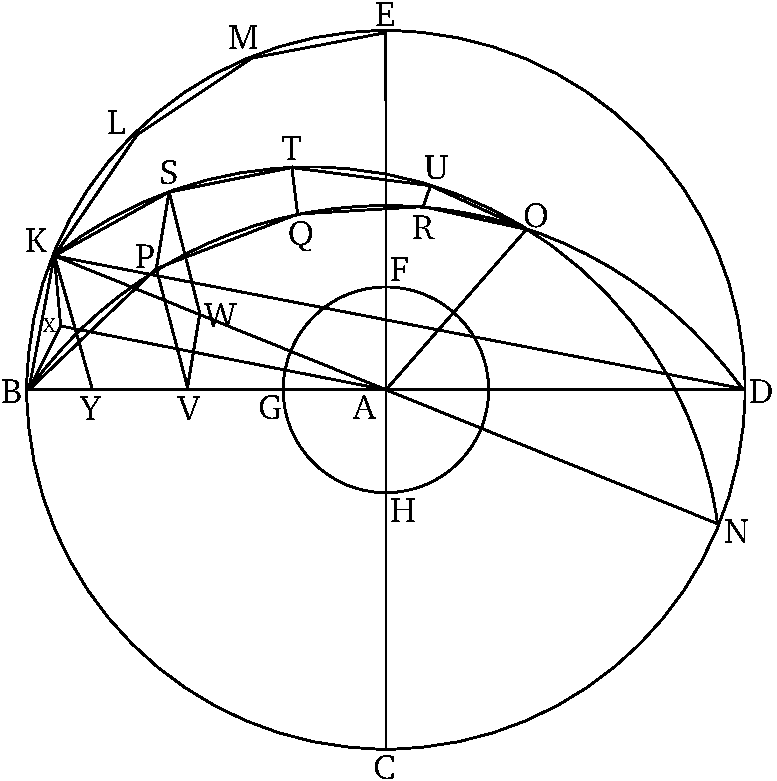
\includegraphics{Book12/fig17e.pdf}}

Let two spheres be conceived about the same center, $A$. So, it is necessary to inscribe a polyhedral solid in the greater
sphere, not touching the lesser sphere on its surface.

Let the spheres be cut by some plane through the center. So, the sections will be circles, inasmuch as a sphere is generated by  the diameter remaining behind,
and a semi-circle being carried around [Def.~11.14]. And, hence,  whatever position we
conceive  (of for) the semi-circle, the  plane produced through it will  make a circle on the surface of the sphere. And (it is) clear
that (it is) also a great (circle), inasmuch as the diameter of the sphere, which is also manifestly the  diameter of  the semi-circle
and the circle, is greater than  all of the (other)  [straight-lines] drawn across in the circle or the sphere [Prop.~3.15]. Therefore, let $BCDE$ be the circle in the greater sphere, and $FGH$ the circle in the lesser sphere. And let two diameters of them be drawn
at right-angles to one another, (namely), $BD$ and $CE$. And there being two circles about the same center---(namely), $BCDE$
and $FGH$---let an equilateral and even-sided polygon be inscribed in the greater circle, $BCDE$, not touching the
lesser circle, $FGH$ [Prop.~12.16], of which let the sides in the quadrant $BE$ be
$BK$, $KL$, $LM$, and $ME$. And, $KA$ being joined, let it be drawn across to $N$. And let $AO$ be
set up at point $A$, at right-angles to the plane of circle $BCDE$. And let it meet the surface of the (greater) sphere at $O$. 
And let planes be produced through  $AO$ and each of $BD$  and $KN$. So, according to the aforementioned (discussion),
they will make great circles on the surface of the (greater) sphere. Let them make (great circles), of which let $BOD$ and $KON$
be semi-circles on the diameters $BD$ and $KN$ (respectively). And since $OA$ is at right-angles
to the plane of circle $BCDE$,  all of the planes through $OA$ are thus also at right-angles to the plane of circle $BCDE$
[Prop.~11.18]. And, hence, the semi-circles $BOD$ and $KON$ are also at right-angles to the
plane of circle $BCDE$. And since semi-circles $BED$, $BOD$, and $KON$ are equal---for (they are) on the
equal diameters $BD$ and $KN$ [Def.~3.1]---the quadrants $BE$, $BO$, and $KO$ are also equal to one another. Thus, as many
sides of the polygon as are in quadrant $BE$, so many are also in quadrants $BO$ and $KO$ equal to the straight-lines
$BK$, $KL$, $LM$, and $ME$. Let them be inscribed, and let them be $BP$, $PQ$, $QR$, $RO$, $KS$,
$ST$, $TU$, and $UO$. And let $SP$, $TQ$, and $UR$ be joined. And let perpendiculars be drawn from
$P$ and $S$ to the plane of circle $BCDE$ [Prop.~11.11]. So, they will fall on the common sections of the planes $BD$ and $KN$ (with $BCDE$),
inasmuch as the planes of $BOD$ and $KON$ are also at right-angles to the plane of circle $BCDE$ [Def.~11.4].
Let them have fallen, and let them be $PV$ and $SW$.  And let $WV$ be joined.  And since  $BP$ and
$KS$ are equal (circumferences) having been cut off  in the equal semi-circles $BOD$ and $KON$ [Def.~3.28], and  $PV$ and $SW$ are
perpendiculars having been drawn (from them), $PV$ is [thus] equal to $SW$, and $BV$ to $KW$ [Props.~3.27, 1.26]. And the whole of
$BA$ is also equal to the whole of $KA$. And, thus, as $BV$ is to $VA$, so $KW$ (is) to $WA$. 
$WV$ is thus parallel to $KB$ [Prop.~6.2]. And since $PV$ and $SW$ are each at right-angles to the plane
of circle $BCDE$,  $PV$ is thus parallel to $SW$ [Prop.~11.6]. And it was also shown (to be) equal to it.
And, thus, $WV$ and $SP$ are equal and parallel [Prop.~1.33]. And since $WV$ is parallel to $SP$,
but $WV$ is parallel to $KB$, $SP$ is thus also parallel to $KB$ [Prop.~11.1]. And  $BP$ and
$KS$ join them. Thus, the quadrilateral $KBPS$ is in one plane, inasmuch as if there are two parallel
straight-lines, and a random point is taken on each of them, then the straight-line joining the points is in the same plane as
the parallel (straight-lines) [Prop.~11.7]. So, for the same (reasons), each of the quadrilaterals
$SPQT$ and $TQRU$ is also in one plane. And triangle $URO$ is also in one plane [Prop.~11.2].
So, if we conceive straight-lines joining points $P$, $S$, $Q$, $T$, $R$,
and $U$ to $A$ then some solid polyhedral  figure will be constructed between the circumferences $BO$ and $KO$,
being composed of pyramids whose bases (are) the quadrilaterals $KBPS$, $SPQT$, $TQRU$, and the triangle $URO$, 
and apex the point $A$. And if we also make the same construction on each of the sides $KL$, $LM$, and $ME$, just as on $BK$, 
and, further, (repeat the construction) in the remaining three quadrants, then some polyhedral figure
which has been inscribed in the sphere will be constructed, being contained by pyramids whose bases (are) the
aforementioned quadrilaterals, and triangle $URO$, and the (quadrilaterals and triangles) similarly arranged
to them, and apex the point $A$.

So, I say that the aforementioned polyhedron  will not touch the lesser sphere on the surface on which  the circle $FGH$ is (situated).

Let the perpendicular (straight-line) $AX$ be drawn from point $A$ to the plane $KBPS$, and let it meet the
plane at point $X$ [Prop.~11.11]. And let $XB$ and $XK$ be joined. And since $AX$ is at right-angles to the plane
of quadrilateral $KBPS$, it is thus also at right-angles to all of the  straight-lines joined to it which are also in the plane of the quadrilateral
[Def.~11.3]. Thus, $AX$ is at right-angles to each of $BX$ and $XK$. And since $AB$ is equal
to $AK$, the (square) on $AB$ is also equal to the (square) on $AK$. And the (sum of the
squares) on $AX$ and $XB$ is equal to the (square) on $AB$. For the angle at $X$ (is) a right-angle [Prop.~1.47]. And the (sum of the squares) on $AX$ and $XK$ is equal to the (square) on
$AK$ [Prop.~1.47]. Thus, the (sum of the squares) on $AX$ and $XB$
is equal to the (sum of the squares) on $AX$ and $XK$. Let the (square) on $AX$ be subtracted from both. Thus, the
remaining (square) on $BX$ is equal to the remaining (square) on $XK$. Thus, $BX$ (is) equal to $XK$. So, similarly,
we can show that  the straight-lines joined from $X$ to $P$ and $S$ are equal to each of $BX$ and $XK$.
Thus, a circle drawn (in the plane of the quadrilateral) with center $X$, and radius one of $XB$ or $XK$, will
also pass through $P$ and $S$, and the quadrilateral $KBPS$ will be inside the circle.

And since $KB$ is greater than $WV$, and $WV$ (is) equal to $SP$, $KB$ (is) thus greater than
$SP$. And $KB$ (is) equal to each of $KS$ and $BP$. Thus, $KS$ and $BP$ are each greater than $SP$. 
And since quadrilateral $KBPS$ is in a circle, and $KB$, $BP$, and $KS$ are equal (to one another), and $PS$ (is) less (than them),
and $BX$ is the radius of the circle, the (square) on $KB$ is thus greater than
double the (square) on $BX$.$^\dag$
Let the perpendicular  $KY$ be drawn from $K$ to $BV$.$^\ddag$ And since $BD$ is less than double
$DY$, and as $BD$ is to $DY$, so the (rectangle contained) by $DB$ and $BY$ (is) to the (rectangle contained) by $DY$
and $YB$---a square being described on $BY$, and a (rectangular) parallelogram (with short side equal to $BY$) completed on $YD$---the (rectangle contained) by $DB$ and $BY$ is thus also less than double the (rectangle contained) by $DY$ and $YB$.
And, $KD$ being joined, the (rectangle contained) by $DB$ and $BY$ is equal to the (square) on $BK$, and the
(rectangle contained) by $DY$ and $YB$ equal to the (square) on $KY$ [Props.~3.31, 6.8~corr.]. Thus, the (square) on $KB$ is  less than double the (square) on $KY$. But, the (square) on $KB$ is greater than
double the (square) on $BX$. 
Thus, the (square) on $KY$ (is) greater than the (square) on $BX$.  And since $BA$ is equal to $KA$, the (square) on $BA$ is
equal to the (square) on $AK$. And the (sum of the squares) on $BX$ and $XA$ is equal to the (square) on $BA$, and
the (sum of the squares) on $KY$ and $YA$ (is) equal to the (square) on 
$KA$   [Prop.~1.47]. 
Thus, the (sum of the squares) on $BX$ and $XA$ is equal to the (sum of the squares) on $KY$ and $YA$, of
which the (square) on $KY$ (is) greater than the (square) on $BX$. Thus, the remaining (square) on $YA$ is less than the
(square) on $XA$. Thus, $AX$ (is) greater than $AY$. Thus, $AX$ is much greater than $AG$.$^\S$ And $AX$ is (a perpendicular) on one of the bases of the
polyhedron, and $AG$ (is a perpendicular) on the surface of the lesser sphere. Hence, the polyhedron will not touch the lesser sphere on its
surface.

Thus, there being two spheres about the same center, a polyhedral solid has been inscribed in the greater sphere which does not
touch the lesser sphere on its surface. (Which is) the very thing it was required to do.}
\end{Parallel}
{\footnotesize\noindent$^\dag$ Since $KB$, $BP$,
and $KS$ are greater than the sides of an inscribed square, which are each of length $\sqrt{2}\,BX$.\\
$^\ddag$ Note that points $Y$ and $V$ are actually identical.\\
$^\S$ This conclusion depends on the fact that the chord of the polygon in proposition 12.16 does not touch the inner circle.}~\\

\begin{Parallel}{}{}
\ParallelLText{
\begin{center}
{\large \gr{Πόρισμα}.}
\end{center}\vspace*{-7pt}

\gr{Ἐὰν δὲ καὶ εἰξ ἑτάραν σφαῖραν τῶ| ἐν τῆ| ΒΓΔΕ σφαίρᾳ στερεῶ| πολυέδρῳ <όμοιον στερεὸν πολύεδρον
ἐγγραφῆ|, τὸ ἐν τῆ| ΒΓΔΕ σφαίρᾳ στερεὸν πολύεδρον πρὸξ τὸ ἐν τῆ| ἑτέρᾳ σφαίρᾳ στερεὸν
πολύεδρον  τριπλασίονα λόγον >έθει, >ήπερ ἡ τῆξ ΒΓΔΕ σφαίραξ διάμετροξ πρὸξ τὴν τῆξ ἑτέραξ σφαίραξ
διάμετρον. διαιρεθέντων γὰρ τῶν στερεῶν εἰξ τὰξ ὁμοιοπληθεῖξ καὶ ὁμοιοταγεῖξ πυραμίδαξ
>έσονται αἱ πυραμίδεξ <όμοιαι. αἱ δὲ <όμοιαι πυραμίδεξ πρὸξ ἀλλήλαξ ἐν τριπλασίονι λόγῳ
εἰσὶ τῶν ὁμολόγων πλευρῶν; ἡ >άρα πυραμίξ, <ῆξ βάσιξ μέν ἐστι τὸ ΚΒΟΣ τετράπλευρον,
κορυφὴ δὲ τὸ Α σημεῖον, πρὸξ τὴν ἐν τῆ| ἑτέρᾳ σφαίρᾳ ὁμοιοταγῆ πυραμίδα τριπλασίονα
λόγον >έθει, >ήπερ ἡ ὁμόλογοξ πλευρὰ πρὸξ τὴν ὁμόλογον πλευράν, τουτέστιν >ήπερ ἡ ΑΒ
ἐκ τοῦ κέντρου τῆξ σφαίραξ τῆξ περὶ κέντρον τὸ Α πρὸξ τὴν ἐκ τοῦ κέντρου τῆξ ἑτέραξ
σφαίραξ. ὁμοίωξ καὶ ἑκάστη πυραμὶξ τῶν ἐν τῆ| περὶ κέντρον τὸ Α σφαίρᾳ πρὸξ ἑκάστην ὁμοταγῆ
πυραμίδα τῶν ἐν τῆ| ἑτέρᾳ σφαίρᾳ τριπλασίονα λόγον
<έχει, >ήπερ ἡ ΑΒ πρὸξ τὴν ἐκ τοῦ κέντρου τῆξ ἑτέραξ
σφαίραξ. καὶ ὡξ <ὲν τῶν ἡγουμένων πρὸξ <ὲν τῶν ἑπομένων, ο<ύτωξ <άπαντα τὰ ἡγούμενα
πρὸξ <άπαντα τὰ ἑπόμενα; <ώστε <όλον τὸ ἐν τῆ| περὶ κέντρον τὸ Α σφαίρᾳ
στερεὸν πολύεδρον πρὸξ <όλον τὸ ἐν τῆ| ἑτέρᾳ [σφαίρᾳ]
στερεὸν πολύεδρον τριπλασίονα λόγον <έχει, >ήπερ ἡ ΑΒ πρὸξ τὴν ἐκ τοῦ κέντρου τῆξ ἑτέραξ
σφαίραξ, τουτέστιν >ήπερ ἡ ΒΔ διάμετροξ πρὸξ τὴν τῆξ ἑτέραξ σφαίραξ διάμετρον; <όπερ >έδει
δεῖχαι.}}

\ParallelRText{
\begin{center}
{\large Corollary}
\end{center}

And, also, if a similar polyhedral solid  to that in sphere $BCDE$ is inscribed in another sphere then the polyhedral solid in sphere $BCDE$ has
to the polyhedral solid in the other sphere the cubed ratio that the diameter of sphere $BCDE$ has to the diameter of the other
sphere. For if the solids are divided into similarly numbered, and similarly situated, pyramids, then the pyramids will be
similar. And similar pyramids are in the cubed ratio of corresponding sides [Prop.~12.8~corr.]. 
Thus, the pyramid whose base is quadrilateral $KBPS$, and apex the point $A$, will have to the similarly situated pyramid in the other
sphere the cubed ratio that a corresponding side (has) to a corresponding side. That is to say, that of radius $AB$ of the
sphere about center $A$ to the radius of the other sphere. And, similarly, each pyramid in the sphere about center $A$ will have to
each similarly situated pyramid in the other sphere the cubed ratio that $AB$ (has) to the radius of the other sphere. And as
one of the leading (magnitudes is) to one of the following (in two sets of proportional magnitudes), so (the sum of) all the
leading (magnitudes is) to (the sum of) all of the following (magnitudes)  [Prop.~5.12]. 
Hence, the whole polyhedral solid in the sphere about center $A$ will have to the whole polyhedral solid in the other [sphere] the
cubed ratio that (radius) $AB$ (has) to the radius of the other sphere. That is to say, that diameter $BD$ (has) to the diameter of the
other sphere. (Which is) the very thing it was required to show.}
\end{Parallel}

%%%%
%12.18
%%%%
\pdfbookmark[1]{Proposition 12.18}{pdf12.18}
\begin{Parallel}{}{}
\ParallelLText{
\begin{center}
{\large \ggn{18}.}
\end{center}\vspace*{-7pt}

\gr{Αἱ σφαῖραι πρὸξ ἀλλήλαξ ἐν τριπλασίονι λόγῳ εἰσὶ τῶν ἰδίων διαμέτρων.}

% Removed epsf size command
\centerline{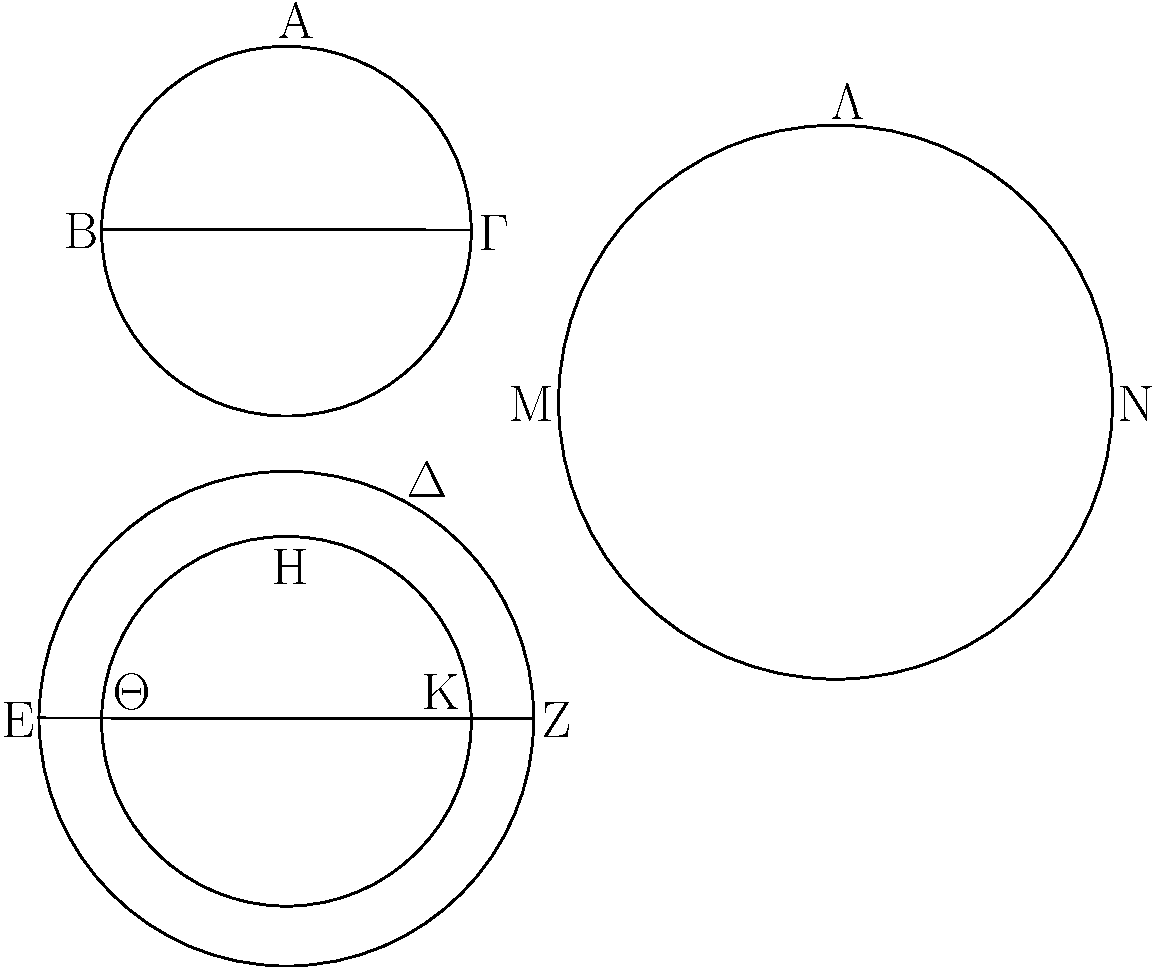
\includegraphics{Book12/fig18g.pdf}}

\gr{Νενοήσθωσαν σφαῖραι αἱ ΑΒΓ, ΔΕΖ, διάμετροι δὲ α\kern -.7pt  ὐτῶν αἱ ΒΓ, ΕΖ; λέγω, <ότι ἡ ΑΒΓ
σφαῖρα πρὸξ τὴν ΔΕΖ σφαῖραν τριπλασίονα λόγον >έθει >ήπερ ἡ ΒΓ πρὸξ τὴν ΕΖ.}

\gr{Εἰ γὰρ μ\kern -.7pt  ὴ ἡ ΑΒΓ σφαῖρα πρὸξ τὴν ΔΕΖ σφαῖραν τριπλασίονα λόγον >έθει >ήπερ
ἡ ΒΓ πρὸξ τὴν ΕΖ, <έχει >άρα ἡ ΑΒΓ σφαῖρα πρὸξ ἐλάσσονά τινα τῆξ ΔΕΖ σφαίραξ
τριπλασίονα λόγον >ὴ πρὸξ μείζονα >ήπερ ἡ ΒΓ πρὸξ τὴν ΕΖ. ἐθέτω πρότερον
πρὸξ ἐλάσσονα τὴν ΗΘΚ, καὶ νενοήσθω ἡ ΔΕΖ τῆ| ΗΘΚ περὶ τὸ α\kern -.7pt  ὐτὸ κέντρον, καὶ
ἐγγεγράφθω εἰξ τὴν μείζονα σφαῖραν τὴν ΔΕΖ στερεὸν πολύεδρον μ\kern -.5pt  ὴ ψα\kern -.3pt  ῦον
τῆξ ἐλάσσονοξ σφαίραξ τῆξ ΗΘΚ κατὰ τὴν ἐπιφάνειαν, ἐγγεγράφθω δὲ καὶ εἰξ
τὴν ΑΒΓ σφαῖραν τῶ| ἐν τῆ| ΔΕΖ σφαίρᾳ στερεῶ| πολυέδρῳ <όμοιον στερεὸν πολύεδρον;
τὸ >άρα ἐν τῆ| ΑΒΓ στερεὸν πολύεδρον πρὸξ τὸ ἐν τῆ| ΔΕΖ στερεὸν πολύεδρον
τριπλασίονα λόγον >έθει >ήπερ ἡ ΒΓ πρὸξ τὴν ΕΖ. >έθει δὲ καὶ ἡ ΑΒΓ σφαῖρα
πρὸξ τὴν ΗΘΚ σφαῖραν τριπλασίονα λόγον >ήπερ ἡ ΒΓ πρὸξ τὴν ΕΖ; >έστιν
>άρα ὡξ ἡ ΑΒΓ σφαῖρα πρὸξ τὴν ΗΘΚ σφαῖραν, ο<ύτωξ τὸ ἐν τῆ| ΑΒΓ σφαίρᾳ
στερεὸν πολύεδρον πρὸξ τὸ ἐν τῆ| ΔΕΖ σφαίρᾳ στερεὸν πολύεδρον; ἐναλλὰχ
[>άρα] ὡξ ἡ ΑΒΓ σφαῖρα πρὸξ τὸ ἐν α\kern -.7pt  ὐτῆ| πολύεδρον, ο<ύτωξ ἡ ΗΘΚ
σφαῖρα πρὸξ τὸ ἐν τῆ| ΔΕΖ σφαίρᾳ στερεὸν πολύεδρον. μείζων δὲ ἡ
ΑΒΓ σφαῖρα τοῦ ἐν α\kern -.7pt  ὐτῆ| πολυέδρου; μείζων
>άρα καὶ ἡ ΗΘΚ σφαῖρα τοῦ ἐν τῆ| ΔΕΖ σφαίρᾳ πολυέδρου. ἀλλὰ καὶ ἐλάττων;
ἐμπεριέθεται γὰρ ὑπ> α\kern -.7pt  ὐτοῦ. οὐκ >άρα ἡ ΑΒΓ σφαῖρα πρὸξ ἐλάσσονα
τῆξ ΔΕΖ σφαίραξ τριπλασίονα λόγον >έθει >ήπερ ἡ ΒΓ διάμετροξ πρὸξ τὴν ΕΖ.
ὁμοίωξ δὴ δείχομεν, <ότι  οὐδὲ ἡ ΔΕΖ σφαῖρα πρὸξ ἐλάσσονα τῆξ ΑΒΓ σφαίραξ
τριπλασίονα λόγον >έθει >ήπερ ἡ ΕΖ πρὸξ τὴν ΒΓ.}

\gr{Λέγω δή, <ότι οὐδὲ ἡ ΑΒΓ σφαῖρα πρὸξ μείζονά τινα τῆξ ΔΕΖ σφαίραξ τριπλασίονα
λόγον >έθει >ήπερ ἡ ΒΓ πρὸξ τὴν ΕΖ.}

\gr{Εἰ γὰρ δυνατόν, ἐθέτω πρὸξ μείζονα τὴν ΛΜΝ; ἀνάπαλιν >άρα ἡ ΛΜΝ σφαῖρα
πρὸξ τὴν ΑΒΓ σφαῖραν τριπλασίονα λόγον >έθει >ήπερ ἡ ΕΖ διάμετροξ πρὸξ τὴν
ΒΓ διάμετρον. 
ὡξ δὲ ἡ ΛΜΝ σφαῖρα πρὸξ τὴν ΑΒΓ σφαῖραν, ο<ύτωξ ἡ ΔΕΖ
σφαῖρα πρὸξ ἐλάσσονά τινα τῆξ ΑΒΓ σφαίραξ, ἐπειδήπερ μείζων
ἐστὶν ἡ ΛΜΝ τῆξ ΔΕΖ, ὡξ >έμπροσθεν ἐδείθθη.
καὶ ἡ ΔΕΖ >άρα σφαῖρα πρὸξ ἐλάσσονά τινα τῆξ ΑΒΓ σφαίραξ
 τριπλασίονα λόγον >έθει >ήπερ ἡ ΕΖ
πρὸξ τὴν ΒΓ; <όπερ ἀδύνατον ἐδείθθη. οὐκ >άρα ἡ ΑΒΓ σφαῖρα πρὸξ
μείζονά τινα τῆξ ΔΕΖ σφαίραξ τριπλασίονα λόγον >έθει >ήπερ ἡ ΒΓ
πρὸξ τὴν ΕΖ. ἐδείθθη δέ, <ότι οὐδὲ πρὸξ ἐλάσσονα. ἡ >άρα ΑΒΓ σφαῖρα
πρὸξ τὴν ΔΕΖ σφαῖραν τριπλασίονα λόγον >έθει >ήπερ ἡ ΒΓ πρὸξ τὴν
ΕΖ; <όπερ >έδει δεῖχαι.}}

\ParallelRText{
\begin{center}
{\large Proposition 18}
\end{center}

Spheres  are to one another in the cubed ratio of their respective diameters.

% Removed epsf size command
\centerline{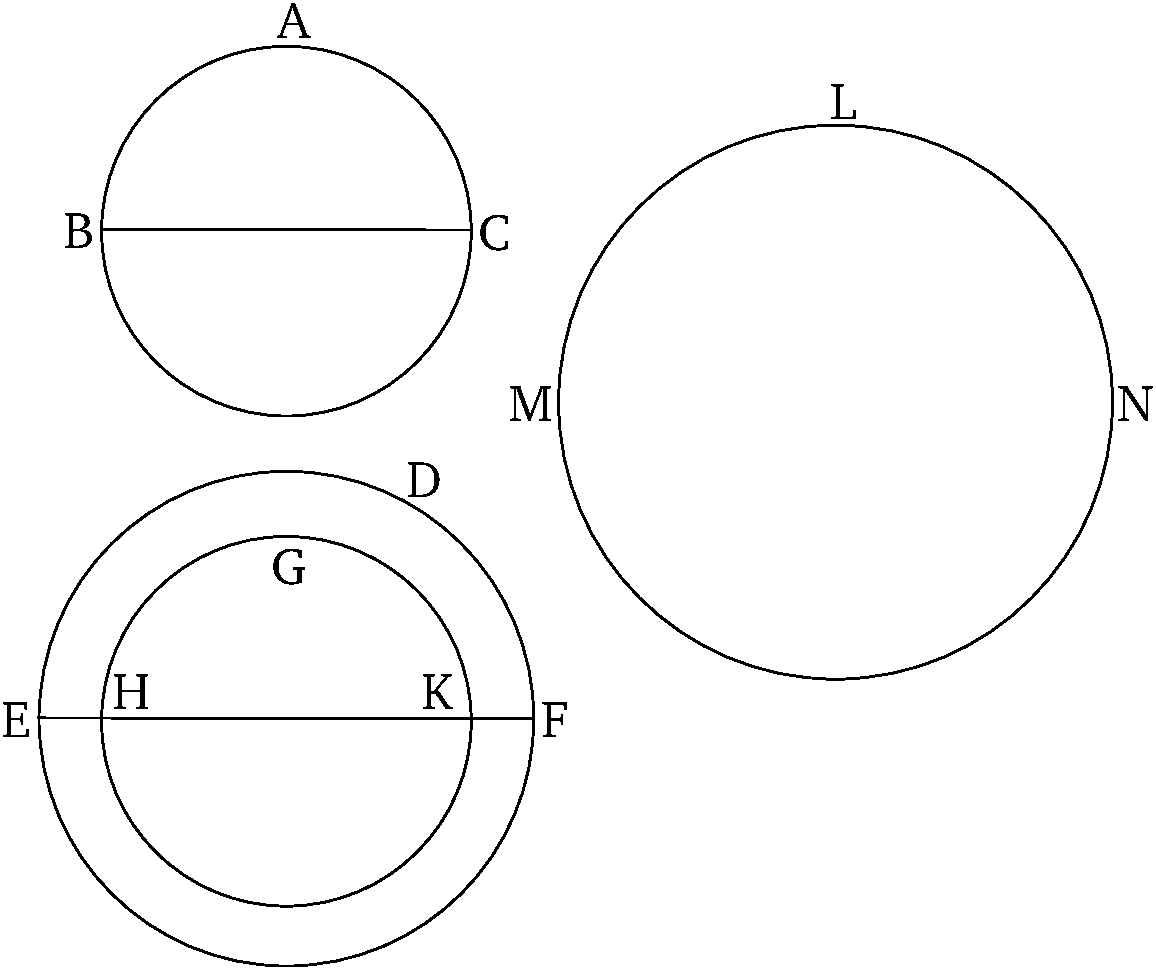
\includegraphics{Book12/fig18e.pdf}}

Let the spheres $ABC$ and $DEF$ be conceived, and (let) their diameters (be) $BC$ and $EF$ (respectively). 
I say that sphere $ABC$ has to sphere $DEF$ the cubed ratio that $BC$ (has) to $EF$.

For if sphere $ABC$ does not have to sphere $DEF$ the cubed ratio that $BC$ (has) to $EF$ then  sphere $ABC$ will have
to some (sphere) either less than, or greater than, sphere $DEF$ the cubed ratio that $BC$ (has) to $EF$.
Let it, first of all, have (such a ratio) to a lesser (sphere), $GHK$. And let $DEF$ be conceived about the same
center as $GHK$. And let a polyhedral solid be inscribed in the greater sphere $DEF$, not touching the lesser
sphere $GHK$ on its surface [Prop.~12.17]. And let a polyhedral solid, similar to the polyhedral
solid in sphere $DEF$, have also been inscribed in sphere $ABC$. Thus, the polyhedral solid in sphere $ABC$ has to
the polyhedral solid in sphere $DEF$ the cubed ratio that $BC$ (has) to $EF$ [Prop.~12.17~corr.].
And sphere $ABC$ also has to sphere $GHK$ the cubed ratio that $BC$ (has) to $EF$.  Thus, as sphere $ABC$
is to sphere $GHK$, so the polyhedral solid in sphere $ABC$ (is) to the polyhedral solid is sphere
$DEF$. [Thus], alternately, as sphere $ABC$ (is) to the polygon within it, so sphere $GHK$ (is) to the polyhedral
solid within sphere $DEF$ [Prop.~5.16]. And sphere $ABC$ (is) greater than the polyhedron
within it. Thus, sphere $GHK$ (is) also greater than the polyhedron within sphere $DEF$ [Prop.~5.14]. But, (it is) also less. For it is encompassed by it. Thus, sphere $ABC$ does not have to (a sphere) less than sphere
$DEF$ the  cubed ratio that diameter $BC$ (has) to $EF$. So, similarly, we can show that sphere
$DEF$ does not have to  (a sphere) less than sphere $ABC$ the cubed ratio 
that $EF$ (has) to $BC$ either.

So, I say that sphere $ABC$ does not have to some (sphere) greater than sphere $DEF$ the cubed ratio that
$BC$ (has) to $EF$ either.

For, if possible, let it have (the cubed ratio) to a greater (sphere), $LMN$. Thus, inversely, sphere $LMN$
(has) to sphere $ABC$ the cubed ratio that diameter $EF$ (has) to diameter $BC$ [Prop.~5.7~corr.].
And as sphere $LMN$ (is) to sphere $ABC$, so sphere $DEF$ (is) to some (sphere) less than sphere $ABC$, inasmuch
as  $LMN$ is greater than $DEF$, as was shown before [Prop.~12.2~lem.]. And, thus, sphere
$DEF$ has to some (sphere) less than sphere $ABC$ the cubed ratio that $EF$ (has) to $BC$. The very thing
was shown (to be) impossible. Thus, sphere $ABC$ does not have to some (sphere) greater than sphere $DEF$
the cubed ratio that $BC$ (has) to $EF$. And it was shown that neither (does it have such a ratio) to a lesser
(sphere). Thus, sphere $ABC$ has to sphere $DEF$ the cubed ratio that $BC$ (has) to $EF$. (Which is)
the very thing it was required to show.}
\end{Parallel}